\documentclass{amsart}
\usepackage{amsmath}
\usepackage{amssymb}
\usepackage{amsthm}
%\usepackage{MnSymbol}
\usepackage{bm}
\usepackage{accents}
\usepackage{mathtools}
\usepackage{tikz}
\usetikzlibrary{calc}
\usetikzlibrary{decorations.pathmorphing,shapes}
\usetikzlibrary{automata,positioning}
\usepackage{tikz-cd}
\usepackage{forest}
\usepackage{braket} 
\usepackage{listings}
\usepackage{mdframed}
\usepackage{verbatim}
\usepackage{physics2}
\usephysicsmodule{ab,ab.legacy,diagmat,xmat}
\usepackage{derivative}
\usepackage{fixdif}
\usepackage{stmaryrd}
% \usepackage{euscript} 
% \usepackage[mathcal]{eucal}
\usepackage{stackengine} 
%\usepackage{/home/patrickl/homework/macaulay2}

%font
\usepackage[sc]{mathpazo}
\usepackage{inconsolata}
\usepackage{microtype}
% \usepackage{fontspec} 
% \setmainfont{Tex Gyre Pagella}
\usepackage[OT1,euler-digits]{eulervm}
% \usepackage{euler-math} 
\usepackage[scaled=0.86]{berasans}
% \let\sffamilyold\sffamily
% \def\sffamily{\fontencoding{T1}\sffamilyold}
% \setmonofont{Inconsolatazi4}

%CS packages
\usepackage{algorithmicx}
\usepackage{algpseudocode}
\usepackage{algorithm}

% typeset and bib
\usepackage[english]{babel} 
% \usepackage[utf8]{inputenc} 
% \usepackage[T1]{fontenc}
% \usepackage[backend=biber,style=alphabetic,maxalphanames=4,maxnames=5,hyperref]{biblatex}
\usepackage[bookmarks, colorlinks, breaklinks]{hyperref} 
\hypersetup{linkcolor=blue,citecolor=magenta,filecolor=black,urlcolor=blue}
\usepackage{cleveref}
\usepackage{graphicx}
\graphicspath{{./}}


% other formatting packages
\usepackage{float}
\usepackage{booktabs}
\usepackage[shortlabels]{enumitem}
\setitemize{noitemsep}
\usepackage{csquotes}
%\usepackage{titlesec}
%\usepackage{titling}
%\usepackage{fancyhdr}
%\usepackage{lastpage}
% \usepackage{parskip}
\newlist{mydescription}{description}{1}
\setlist[mydescription]{style=nextline,
                        font=\bfseries,
                        % Tweak the next 4 options as needed:
                        labelindent=1cm, 
                        leftmargin =2cm,
                        rightmargin=1cm,
                        topsep     =1ex
                       }
\setcounter{tocdepth}{1}
\usepackage{lipsum}

% delimiters
\DeclarePairedDelimiter{\gen}{\langle}{\rangle}
\DeclarePairedDelimiter{\floor}{\lfloor}{\rfloor}
\DeclarePairedDelimiter{\ceil}{\lceil}{\rceil}


\newtheorem{thm}{Theorem}[section]
\newtheorem{cor}[thm]{Corollary}
\newtheorem{prop}[thm]{Proposition}
\newtheorem{lem}[thm]{Lemma}
\newtheorem{conj}[thm]{Conjecture}
\newtheorem{quest}[thm]{Question}
\newtheorem{claim}[thm]{Claim}

\theoremstyle{definition}
\newtheorem{defn}[thm]{Definition}
\newtheorem{defns}[thm]{Definitions}
\newtheorem{con}[thm]{Construction}
\newtheorem{exm}[thm]{Example}
\newtheorem{exms}[thm]{Examples}
\newtheorem{notn}[thm]{Notation}
\newtheorem{notns}[thm]{Notations}
\newtheorem{addm}[thm]{Addendum}
\newtheorem{exer}[thm]{Exercise}

\theoremstyle{remark}
\newtheorem{rmk}[thm]{Remark}
\newtheorem{rmks}[thm]{Remarks}
\newtheorem{warn}[thm]{Warning}
\newtheorem{sch}[thm]{Scholium}


% unnumbered theorems
\theoremstyle{plain}
\newtheorem*{thm*}{Theorem}
\newtheorem*{prop*}{Proposition}
\newtheorem*{lem*}{Lemma}
\newtheorem*{cor*}{Corollary}
\newtheorem*{conj*}{Conjecture}

% unnumbered definitions
\theoremstyle{definition}
\newtheorem*{defn*}{Definition}
\newtheorem*{exer*}{Exercise}
\newtheorem*{defns*}{Definitions}
\newtheorem*{con*}{Construction}
\newtheorem*{exm*}{Example}
\newtheorem*{exms*}{Examples}
\newtheorem*{notn*}{Notation}
\newtheorem*{notns*}{Notations}
\newtheorem*{addm*}{Addendum}


\theoremstyle{remark}
\newtheorem*{rmk*}{Remark}

% shortcuts
\DeclareMathOperator{\Ima}{Im}
\newcommand{\A}{\mathbb{A}}
\newcommand{\G}{\mathbb{G}}
\newcommand{\N}{\mathbb{N}}
\newcommand{\R}{\mathbb{R}}
\newcommand{\C}{\mathbb{C}}
\newcommand{\Z}{\mathbb{Z}}
\newcommand{\Q}{\mathbb{Q}}
\newcommand{\E}{\mathbb{E}}
\newcommand{\V}{\mathbb{V}}
\renewcommand{\H}{\mathbb{H}}
\renewcommand{\k}{\Bbbk}
\renewcommand{\L}{\mathbb{L}}
\renewcommand{\P}{\mathbb{P}}
\newcommand{\M}{\mathcal{M}}
\newcommand{\Mbar}{\overline{\mathcal{M}}}
\newcommand{\g}{\mathfrak{g}}
\newcommand{\h}{\mathfrak{h}}
\newcommand{\n}{\mathfrak{n}}
\renewcommand{\b}{\mathfrak{b}}
\newcommand{\ep}{\varepsilon}
\newcommand*{\dt}[1]{%
   \accentset{\mbox{\Huge\bfseries .}}{#1}}
%\renewcommand{\abstractname}{Official Description}
\newcommand{\mc}[1]{\mathcal{#1}}
% \newcommand{\msc}[1]{\mathscr{#1}}
\newcommand{\T}{\mathbb{T}}
\newcommand{\mf}[1]{\mathfrak{#1}}
\newcommand{\mbf}[1]{\mathbf{#1}}
\newcommand{\bv}{\mbf{v}}
\newcommand{\bq}{\mbf{q}}
\newcommand{\bp}{\mbf{p}}
\newcommand{\btau}{\bm{\tau}}
\newcommand{\mr}[1]{\mathrm{#1}}
\newcommand{\on}[1]{\operatorname{#1}}
\newcommand{\ms}[1]{\mathsf{#1}}
\newcommand{\mt}[1]{\mathtt{#1}}
\newcommand{\ol}[1]{\overline{#1}}
\newcommand{\ul}[1]{\underline{#1}}
\newcommand{\wt}[1]{\widetilde{#1}}
\newcommand{\wh}[1]{\widehat{#1}}
\renewcommand{\div}{\operatorname{div}}
\newcommand{\1}{\mathbf{1}}
\newcommand{\2}{\mathbf{2}}
\newcommand{\3}{\mathbf{3}}
\newcommand{\I}{\mathrm{I}}
\newcommand{\II}{\mr{I}\hspace{-1.3pt}\mr{I}}
\newcommand{\III}{\mr{I}\hspace{-1.3pt}\mr{I}\hspace{-1.3pt}\mr{I}}
\renewcommand{\v}{\mbf{v}}
\newcommand{\w}{\mbf{w}}
\newcommand{\bmu}{\bm{\mu}}
\newcommand{\pre}{\mr{pre}}
\newcommand{\vir}{\mr{vir}}
\newcommand{\fl}{\mr{fl}}
\newcommand{\ps}[1]{\llbracket #1 \rrbracket}
\newcommand{\ls}[1]{\llparenthesis #1 \rrparenthesis}
\newcommand{\loc}{\mr{loc}}

\DeclareMathOperator{\Der}{Der}
\DeclareMathOperator{\Tor}{Tor}
\DeclareMathOperator{\Hom}{Hom}
\DeclareMathOperator{\End}{End}
\DeclareMathOperator{\Ext}{Ext}
\DeclareMathOperator{\ad}{ad}
\DeclareMathOperator{\Aut}{Aut}
\DeclareMathOperator{\Rad}{Rad}
\DeclareMathOperator{\Pic}{Pic}
\DeclareMathOperator{\NS}{NS}
\DeclareMathOperator{\supp}{supp}
\DeclareMathOperator{\Supp}{Supp}
\DeclareMathOperator{\depth}{depth}
\DeclareMathOperator{\sgn}{sgn}
\DeclareMathOperator{\spec}{Spec}
\DeclareMathOperator{\Spec}{Spec}
\DeclareMathOperator{\proj}{Proj}
\DeclareMathOperator{\Proj}{Proj}
\DeclareMathOperator{\ord}{ord}
\DeclareMathOperator{\Div}{Div}
\DeclareMathOperator{\Bl}{Bl}
\DeclareMathOperator{\coker}{coker}
\DeclareMathOperator{\ev}{ev}
\DeclareMathOperator{\st}{st}
\DeclareMathOperator{\pr}{pr}
\DeclareMathOperator{\ch}{ch}
\DeclareMathOperator{\Cont}{Cont}

% \addbibresource{../../notes/math.bib}

\title{Log GLSM and related topics}
\author{Patrick Lei}
\date{\today}
\allowdisplaybreaks

\begin{document}
    
\begin{abstract}
    These are notes from the log GLSM summer school at Sichuan University in July 2026.
\end{abstract}

\maketitle

\tableofcontents

\section{Theta-stratifications (Yaoxiong Wen and Bin Wang)}%
\label{sec:Theta-stratifications}

\subsection{Our first moduli problems}%
\label{sub:Our first moduli problem}

Our first moduli space will be \(\P^{N-1}\), which parameterizes \(1\)-dimensional linear subspaces in \(\C^n\), or equivalently is \((\C^N \setminus 0) / \C^{\times}\), which here means the set of closed orbits of \(\C^{\times}\). This construction is our first example of geometric invariant theory. In general, a moduli problem will assign to every scheme \(T\) a collection of families over \(T\), and we can think of it as a functor
\[ F \colon (\ms{Sch}_{/S})^{\mr{op}} \to \ms{Set}. \]

\begin{exm}
    Let \(C\) be a smooth projective curve. Then consider the assignment
    \[ F_{r,d} \colon T \mapsto \ab\{ E \text{ vector bundle on } C \times T \mid \on{rk} E = r, \deg E = d \}/\sim, \]
    which parameterizes vector bundles on \(C\) (but not quite correct). 
\end{exm}

\begin{exm}
    By the Yoneda Lemma, every scheme \(Y\) defines a moduli problem.
\end{exm}

Unfortunately, not every moduli problem is representable by a scheme or algebraic space, for example if it has automorphisms. For example, if we consider the moduli of line bundles on \(\P^1\), each object has an entire \(\C^{\times}\) of automorphisms. Therefore, when we consider moduli problems, we will also need to consider isomorphisms between the objects (and therefore the target of the functor should be the ategory of groupoids).

\begin{defn}[informal]
    A \textit{stack} \(\mf{X}\) is a functor
    \[ (\ms{Sch}_{/S})^{\mr{op}} \to \ms{Grpd}. \]
\end{defn}

\begin{exm}
    Consider the stack \(\ms{Bun}_{r,d}(C)\) which sends a scheme \(T\) to the groupoid of vector bundles of rank \(r\) and degree \(d\) on \(T \times C\).     
\end{exm}

Unfortunately, there are far too many stacks to consider, so we will need to consider a subclass of stacks which is amenable to the methods of algebraic geometry.

\begin{defn}
    An \textit{algebraic stack} is a stack with representable (by algebraic spaces) diagonal and with a smooth surjective morphism from a scheme \(U\) (which is called an atlas). 
\end{defn}

Note that the first condition means that for any morphism \(T \to \mf{X} \times \mf{X}\) from an algebraic space, then \(T \times_{\mf{X} \times \mf{X}} \mf{X}\) is an algebraic space. This is equivalent to all Isom sheaves being algebraic spaces and implies that any morphism from a scheme to \(\mf{X}\) is representable.

\begin{rmk}
    In the classical setting, if we have morphisms \(f\colon A \to C\) and \(g \colon B \to C\), then the fiber product is
    \[ A \times_C B = \ab\{(a,b) \mid f(a) = g(b) \}. \]
    However, in the setting of stacks, we need to replace equality by isomorphism, but this implies that we need to actually record the isomorphism.
\end{rmk}

\subsection{Quotient stacks}%
\label{sub:Quotient stacks}

Let \(G\) be an algebraic group an \(X\) be a scheme with an action of \(G\).

\begin{defn}
    The \textit{quotient stack} \([X/G]\) sends a stack \(T\) to the groupoid which consists of diagrams
    \begin{equation*}
    \begin{tikzcd}
        P \ar{r}{\varphi} \ar{d} & X \\
        T
    \end{tikzcd}
    \end{equation*}
    where \(P\) is a principal \(G\)-bundle over \(T\) and \(\varphi\) is an equivariant morphism.   
\end{defn}

\begin{exm}
    Any smooth separated DM stack with either generically trivial stabilizer or quasi-projective coarse moduli space is a global quotient. Here, a DM stack is an algebraic stack with unramified diagonal.
\end{exm}

\begin{exer}
    Show that the groupoid \([X/G](\C)\) is equivalent to the action groupoid of \(G(\C)\) acting on \(X(\C)\).
\end{exer}

The above exercise implies that as a groupoid (most importantly, not as an algebraic stack), we have
\[ [X/G](\C) \simeq \bigsqcup_{[x_i] \in X(\C)/G(\C)} BG_{x_i}. \]

\subsection{Fine vs coarse vs good moduli spaces}%
\label{sub:Fine vs coarse vs good moduli spaces}

\begin{defn}
    A \textit{fine moduli space} for a moduli problem is a scheme or algebraic space \(M\) which represents the functor. 
\end{defn}

Unfortunately, it is very hard to find a fine moduli space, so we want to weaken this condition.

\begin{defn}
    A \textit{coarse moduli space} \(M\) for an algebraic stack \(\mf{X}\) is a morphism \(\pi \colon \mf{X} \to M\) such that
    \begin{enumerate}
        \item \(\pi\) is universal for morphisms from \(\mf{X}\) to algebraic spaces;
        \item \(\pi\) is bijective on geometric points.
    \end{enumerate}
\end{defn}

Even these do not always exist, so we consider an even weaker notion.

\begin{defn}
    A \textit{good moduli space} \(q \colon \mf{X} \to X\) is a \textit{good moduli space} if
    \begin{enumerate}
        \item The pushforward functor \(q_* \colon \ms{QCoh}(\mf{X}) \to \ms{QCoh}(X)\) is exact;
        \item The natural map \(\mc{O}_X \to q_* \mc{O}_{\mf{X}}\) is an isomorphism.
    \end{enumerate}
\end{defn}

\begin{table}[htpb]
    \centering
    \caption{Types of moduli spaces}
    \label{tab:moduli-types}
    \begin{tabular}{cccc}
        \toprule
        Can handle & finite stabilizer & infinite stabilizer & feature \\
        \midrule
        Fine moduli & No & No & Admits universal family \\
        Coarse moduli & Yes & No & Bijection on points \\
        Good moduli & Yes & Yes & S-equivalence \\
        \bottomrule
    \end{tabular}
\end{table}

\begin{thm}[Keel-Mori]
    Let \(\mf{X}\) be an algebraic stack which has finite inertia. Then it has a coarse moduli space. 
\end{thm}

\begin{thm}[Alper]
    \dots\dots\footnote{Yaoxiong literally wrote this on the board.}
\end{thm}

Unfortunately the stack \(\ms{Bun}_{r,d}(C)\) is ``too big to be good,'' namely that it is not quasi-compact and non-separated. For example, we can consider a vector bundle \(E_r = L_n \oplus M_{d-n} \oplus \mc{O}^{\bigoplus r-2}\), then send \(n \to \infty\), so this clearly cannot satisfy any finiteness condition. To see why this stack is non-separated, note that if \(E\) is a stable bundle, it has automorphisms given by \(\C^{\times}\), which is not proper. To fix this problem, we will study an open substack of semistable objects and then consider S-equivalence classes.

\begin{defn}[Slope stability]
    Define the quantity
    \[ \mu(E) = \frac{\deg E}{\on{rk} E}. \]
    E is \textit{(semi)stable} if for any proper subbundle \(F \subset E\), we have \(\mu(F) \leq \mu(E)\) or \(\mu(F) < \mu(E)\), respectively.   
\end{defn}

Armed this definition, we may now consider the substack \(\ms{Bun}_{r,d}^{\mr{ss}}(C)\), which is quasi-compact but still not separated (because of the problem of automorphisms).

\begin{defn}[S-equivalence]
    Two vector bundles \(E\) and \(E'\) are \textit{S-equivalent} if they have the same associated graded pieces of their Jordan-Holder filtration. Here, the Jordan-Holder filtration is a filtration
    \[ 0 = J_0 \subset J_1 \subset \cdots \subset J_N = E \]
    such that all \(J_i / J_{i=1}\) are stable. While the filtration is not necessarily unique, the associated graded is unique.
\end{defn}

Now we consider the moduli space \(M_{r,d}^{\mr{ss}}(C)\) be the moduli space of S-equivalence classes of semistable vector bundles on \(C\). The morphism \(\ms{Bun}_{r,d}^{\mr{ss}}(C) \to M_{r,d}^{\mr{ss}}(C)\) is a good moduli space.

\begin{rmk}
    The original method of proof for this theorem was to construct the moduli space using geometric invariant theory. The goal of this series of lectures will be to discuss how to prove this type of theorem without making reference to GIT.
\end{rmk}

\subsection{Theta-stratifications}%
\label{sub:Theta-stratifications}

Let \(\mf{X}\) be an algebraic stack and consider \(\Theta \coloneqq [\A^1 / \G_m]\). Then define the stack \(\ms{Filt}(\mf{X}) \coloneqq \ms{Map}(\Theta, \mf{X})\) of filtered objects and the stack \(\ms{Grad}(\mf{X}) \coloneqq \ms{Map}(B\G_m, \mf{X})\) of graded objects.    

\begin{defn}
    A \textit{\(\Theta\)-stratification} of \(\mf{X}\) consists of
    \begin{enumerate}
        \item A totally ordered set \(I\);
        \item For all \(\alpha \in I\) an open substack \(\mf{X}_{\leq \alpha} \subset \mf{X}\);
        \item For all \(\alpha \in I\), a \(\Theta\)-stratum \(S_{\alpha} \subset \ms{Filt}(\mf{X}_{\leq \alpha})\) such that
            \[ X_{<\alpha} = \bigcup_{\beta < \alpha} \mf{X}_{\leq \beta} = X_{\leq \alpha} \setminus \ev_1(S_{\alpha}). \]
            This implies \(\mf{X} = \mf{X}^{\mr{ss}}\sqcup \bigsqcup_{\alpha} \ev_1(S_{\alpha})\). 
    \end{enumerate}
    Here a \(\Theta\)-stratum is a union of connected components of \(\ms{Filt}( \mf{X}_{\leq \alpha} )\) such that \(\ev_1(S_{\alpha})\) is a closed substack.  
\end{defn}

Consider the stack \(\ms{Bun}_G(C) = \ms{Map}(C, BG)\). We will consider the stack
\[ \ms{Map}(\Theta, \ms{Bun}_G(C)) = \ms{Map}(\Theta \times C, BG). \]
Any such map \(f\) is equivalent to a \(\G_m\)-equivariant principal G-bundle \(\mc{E}\) over \(\A^1 \times \C\), which when \(G = \on{GL}_n\) is equivalent to a graded \(\mc{O}_C\)-module. Here, we will take \(t\) to have weight \(1\). By flatness of \(\mc{E}\), the map \(t \colon \mc{E}_w \to \mc{E}_{w+1}\) is injective.    

\begin{rmk}
    Consider the vector bundle \(E = \mf{E}_{|1 \times C}\). Then \(\mc{E}_{|(\G_m \times C)} = P_C^* E\), where \(P_C \colon C \times \G_m \to C\) is the projection to the first factor and thus \(E = \mc{E}[t^{-1}]_0\). Defining \(F^w E = \mc{E}_w \cdot t^{-w} \subset E\), we see that \(F^w E \subset F^{w+1} E\). This gives us a filtration
    \[ 0 \subset \cdots \subset F^w E \subset F^{w+1} E \subset \cdots \subset E. \]

    In the other direction, we will require the Rees construction which sends a vector bundle \(E\) with filtration \(F^{\bullet}\) a module
    \[ \ms{Rees}(E, F^{\bullet}) \sum_w t^{-w} F^w E \subset E \otimes_{\C} \C[t, t^{-1}]. \]
\end{rmk}

Therefore, a map from \(\Theta\) to the stack of vector bundles is simply a filtration on a vector bundle.

\subsection{Non-abelian localization}%
\label{sub:Non-abelian localization}

We will begin with the classical setting. Let \(X\) be a smooth projective variety with an action on \(\G_m\). Then let \(X^{\G_m} = \sqcup_{\alpha}Z_{\alpha}\). We can then compute equivariant Euler characteristics as
\[ \chi_{\G_m}(X, F) = \sum_{\alpha} \chi_{\G_m} \ab(Z_{\alpha}, \frac{F_{|Z_{\alpha}}}{e(N_{Z_{\alpha}/X})}), \]
where
\[ e(N_{Z_{\alpha}/X}) = \lambda_{-1}(N_{Z_{\alpha}/Z}^{\vee}) = \sum (-1)^i [\Lambda^i N_{Z_{\alpha}/X}^{\vee}]. \]

We will now consider the stacky version. Let \(\mf{X} = \mf{X}^{\mr{ss}} \sqcup \bigsqcup S_{\alpha}\) be a \(\Theta\)-stratification and \(Z_{\alpha} = \sigma^{-1}(S_{\alpha})\), where \(\sigma \colon \ms{Grad}(\mf{X} \to \ms{Filt}(\mf{X}))\) is the projection \(\Theta \to B\G_m\).

\begin{thm}
    Let \(\mf{X}\) be a quasi-smooth derived stack and \(F \in \ms{Perf}(\mf{X})\) satisfy various conditions. Then
    \[ \chi(\mf{X}, F) = \chi(\mf{X}^{\mr{ss}}, F) + \sum_{\alpha} \chi(Z_{\alpha}, F_{|_{Z_{\alpha}}} \otimes \E_{\alpha}). \]
    Here, if we split \(\L_{\mf{X},|Z_{\alpha}} = \L_{\alpha}^+ \oplus \L_{\alpha}^-\), we have
    \[ E_{\alpha} = \on{Sym}(\L_{\alpha}^- \oplus (\L_{\alpha}^+)^{\vee}) \otimes \det (L_{\alpha}^+)^{\vee}[-\on{rk}(\L_{\alpha}^+)]. \]
\end{thm}

\subsection{Geometric invariant theory}%
\label{sub:Geometric invariant theory}

Let \(G\) be a reductive group and \(X\) be a projective scheme equipped with a \(G\)-equivariant line bundle \(\mc{L}\). The semistable locus can be defined using the Hilbert-Mumford criterion, where it consists of all points where for all cocharacters
\(\lambda \colon \G_m \to G\), we can define the point 
\[ x_0 = \lim_{t \to 0} \lambda(t) x \]
and define the quantity
\[ \mu^L(x, \lambda) \coloneqq \frac{-\on{wt}_{x_0}(\mc{L})}{\norm{\lambda}}. \]
A point is semistable if \(\mu^L(x, \lambda) \leq 0\) for all cocharacters of \(G\). The stable locus consists of all points where the inequality is strict and the stabilizer is finite.

\begin{thm}
    The stable and semistable loci are open in \(X\). Moreover, \(X^{\on{ss}}/G\) is a good quotient and \(X^s/G\) is a geometric quotient.  
\end{thm}

\begin{exm}
    Consider the moduli stack \(\ms{Bun}_{r,d}\) of vector bundles of rank \(r\) and degree \(d\) on a curve of genus at least \(@\). Then recall that the semistable locus was defined to consist of slope semistable vector bundles. In fact, this can be obtained via GIT.

    Fix an ample line bundle \(\mc{O}(1)\) on \(C\). Then there exists some \(n_0\) such that for all \(n \geq n_0\) and \(E \in \ms{Bun}_{r,d}\), \(E(n)\) is globally generated. Therefore, we can consider
    \[ H^0(C, E(n)) \twoheadrightarrow E(n). \]
    If we set \(V = \C^N\), where \(N = h^0(E(n))\), then there is a surjection
    \[ V \otimes_{\mc{O}_C(-n)} \twoheadrightarrow E. \]
    Therefore, we can think of \(E\) as a member of a Quot scheme. On the Quot scheme, we can consider the universal family
    \begin{equation*}
    \begin{tikzcd}
        V \otimes \mc{O}_C(-n) \ar[twoheadrightarrow]{r} \ar{d} & \mc{E} \\
        \ms{Quot}_{V \otimes \mc{O}_C(-n), p_E} \times C \ar{r}{p} & \ms{Quot}_{V \otimes \mc{O}_C(-n)}.
    \end{tikzcd}
    \end{equation*}
    Now define the line bundle
    \[ \mc{L} \coloneqq \det R^0 p_* (\mc{E}(m)) \]
    for some \(m \gg 0\). We can also consider the action of \(\mr{SL}(V)\) on the Quot scheme. For some cocharacter \(\lambda\), we can split
    \[ V = V_1 \oplus V_2 \]
    with weights \(s\) and \(N-s\). 
    Then consider
    \[ V_1 \otimes \mc{O}_C(-n) \subset V \otimes \mc{O}_C(-n) \twoheadrightarrow E \]
    and consider the filtration
    \[ 0 \to F^1 E \to E \to E / F^1 E \to 0 \]
    induced by this. Then we see that 
    \[ \lim_{t \to 0} \lambda(t) E = F^1 E \oplus E/F^1 E. \]
    Then we compute the restriction \(\mc{L}_{|\on{gr}_F E}\) and obtain the spaces \(H^0(C, F^1 E(m))\) and \(H^0(C, E(m)/F^1 E(m))\), and therefore the weight of \(\mc{L}\) is given by
    \[ (N-s) p_{F^1 E}(m) - s p_{E/F^1 E}(m), \]
    which recovers GIT.
\end{exm}

We will now consider the unstable locus. Let \(E\) be a vector bundle on \(C\). Then there exists a unique filtration
\[ 0 \subset F^{\ell} E \subseteq \cdots \subseteq F^0 E = E \]
such that
\begin{enumerate}
    \item All \(\on{gr}_F E\) are semistable;
    \item We have \(\mu(\on{gr}_F^i E) > \mu(\on{gr}_F^{i-1} E)\) for all \(i\). 
\end{enumerate}
\begin{rmk}
    From the GIT perspective, we should really take \(\mu\) to be the reduced Hilbert polynomial.
\end{rmk}

\subsection{Construction of Theta-stratifications}%
\label{sub:Construction of Theta-stratifications}

Let \(\mf{X}\) be a reasonable algebraic stack.\footnote{Here, reasonable means something like locally of finite presentation with qcqs diagonal.} Now consider some family \(\mc{E}\) over \(\A^1 \times C\). If we restrict to the central fiber, we see that \(\G_m\) acts on \(\on{gr}_F E\), which means we have a map \(\G_m \to \Aut \on{gr}_F E\), and from this we can compute the weight from this. 

Note that the morphism \(\sigma \colon \ms{Grad}(\mf{X}) \to \ms{Filt}(\mf{X})\) is a \(\Theta\)-contraction, and therefore
\[ \pi_0(\ms{Filt}(\mf{X})) = \pi_0(\ms{Grad}(\mf{X})). \]

\begin{exm}
    Let \(\mf{X} = BG\). Then we have
    \[\ms{Filt}(\mf{X}) = \bigsqcup_{[\lambda]} B P_{\lambda}, \]
    where \(P_{\lambda}\) is the parabolic subgroup corresponding to the cocharacter \(\lambda\), and we can always choose representatives in a single Weyl chamber. Moreover, we have
    \[ \ms{Grad}(\mf{X}) = \bigsqcup_{\lambda \in \mathbb{X}_*(T)/W} B L_{\lambda}, \]
    where \(L_{\lambda}\) is the Levi subgroup corresponding to \(\lambda\).
\end{exm}

\begin{defn}
    A \textit{\(\Theta\)-stratum} in \(\mf{X}\) is a union of connected components \(S \subseteq \ms{Filt}(\mf{X})\) such that
    \[ \ev_1 \colon S \to \mf{X} \]
    is a closed immersion.
\end{defn}

Roughly speaking, closed immersions are injective, so an object in \(S\) consists of an object in \(\mf{X}\) and a ``canonical filtration.''

\begin{defn}
    A \textit{\(\Theta\)-stratification} is an increasing family of open substacks
    \[ \mf{X}_{\leq c} \subseteq \mf{X}, \qquad c \in \Gamma, \]
    where \(\Gamma\) is some totally ordered set, together with \(\Theta\)-strata
    \[ S_c \subseteq \ms{Filt}(\mf{X}_{\leq C}), \]
    which are required to satisfy
    \[ \mf{X}_{\leq c} = \ev_1(S_c) \sqcup \bigcup_{c' < c} \mf{X}_{\leq c'}. \]
    In particular, this implies that
    \[ \mf{X} = \mf{X}^{\mr{ss}} \sqcup \bigsqcup_{c > 0} \ev_1(S_c). \]
\end{defn}

Analogously to the Hilbert-Mumford criterion, we will construct \(\Theta\)-stratifications using numerical invariants.
\begin{defn}
    A \textit{numerical invariant} \(\mu\) with values in a totally ordered set \(\Gamma\) consists of an assignment of a scaling invariant function
    \[ \mu \colon \R^q \setminus \ab\{0\} \to \Gamma \]
    for any \(p \in \mf{X}(\C)\) and any nondegenerate homomorphism \(\gamma \colon \G_m^q \to \Aut(p)\). These are required to satisfy
    \begin{enumerate}
        \item The assignment is invariant under field extensions. This point will not be elaborated on because we are working over \(\C\);
        \item If we have \(\G_m^q \hookrightarrow \G_m^n \hookrightarrow \Aut(p)\), then we have a factorization \(\R^q \setminus \ab\{0\} \to \R^n \setminus \{0\} \to \Gamma\);
        \item If we have some \(\xi \colon S \to \mf{X}\) and \(\gamma \colon \G_{m, S}^q \to \Aut(\xi)\) with finite kernel, the function \(\mu_{\kappa(s)}\) is locally constant on \(S\), where \(s\) ranges over points of \(S\).
    \end{enumerate}
\end{defn}

We will give a naive version of a construction starting with a numerical invariant \(\mu\). Define \(x \in \mf{X}\) to be semistable if \(\mu(f) \leq 0\) for any nondegenerate \(f \in \ms{Filt}(\mf{X})\) satisfying \(f(1) = x\). If \(x\) is unstable, then we define its instability level
\[ M^{\mu}(x) \coloneqq \sup \ab\{ \mu(f) \mid f \in \ms{Filt}(\mf{X}), \ev_1(f) = x.\} \]
If a filtration \(f\) attains this supremum, we call it a ``Harder-Narasimhan filtration.''

\begin{defn}
    A numerical invariant \(\mu\) is \textit{standard} if
    \begin{enumerate}
        \item \(\mu(x)\) and \(\mu(-x)\) are not both possitive for \(x \in \R^q \setminus \ab\{0\}\);
        \item Each function \(\mu_{\gamma}\) is strictly quasi-concave, namely for all \(\delta \in [0,1]\) and linearly independent \(x_0, x_1 \in \R^q\) such that \(\mu(x_0), \mu(x_1) \geq 0\), then 
            \[\mu_{\gamma}(\delta x_0 + (1-\delta)x_1) \geq \max\ab\{\mu_{\gamma}(x_0), \mu_{\gamma}(x_1)\}.\] If either value is strictly positive, the inequality is required to be strict.
    \end{enumerate}
\end{defn}

The next condition is that we need some kind of rationality. We can see \(\mathbb{X}_*(T)_{\R}\), and our goal is to find the rational points. This leads us to condition (R): If for any \(\gamma\) for which \(\mu_{\gamma}\) attains a positive value, then it attains a maximal value at a rational point.

\begin{thm}
    Let \(\mf{X}\) be a stack and \(\mu\) be a standard numerical invariant satisfying condition (R). Then \(\mu\) defines a \(\Theta\)-stratification if and only if it satisfies the following:
    \begin{itemize}
        \item For any DVR \(R\) with fraction field \(K\) and residue field \(k\), then \(\mu(f_K^{\mr{HN}}) \leq M^{\mu}(f_k)\) (HN-specialization);
        \item For any map \(B \colon T \to \mf{X}\) from a finite type scheme, there exists a quasi-compact open \(\mf{X}' \subseteq \mf{X}\) such that for any point of finite type \(p \in T(k)\) and a filtration \(f\) of \(B(p)\) for which \(\mu(f) > 0\), there exists another filtration \(f'\) of \(B(p)\) with \(\mu(f') \geq \mu(f)\) satisfying \(f'(0) \in \mf{X}'\) (HN-boundedness).
    \end{itemize}
\end{thm}

The point here is that the conditions of being standard and (R) combined with HN-boundedness imply existence and HN-specialization implies uniqueness.



\section{Intro to log geometry (Tingting Fang and Zijian Han)}%
\label{sec:Intro to log geometry (Tingting Fang and Zijian Han)}

\subsection{Motivation}%
\label{sub:Motivation}

In enumerative geometry, we will consider intersection numbers on compactified moduli spaces. This is going to require our objects to degenerate in some way, for example for domain curves to be nodal, maps to land in boundary divisors, or we degenerate the target. In ordinary geometry, we view these as singular, but in log geometry, there is a way to think of these situations as being \textit{log smooth}. In log geometry, we are going to replace functions with the data of functions and how they vanish on the boundary (or namely the morphism \(\alpha \colon M_X \to \mc{O}_X\)).

\begin{exm}
    Consider a family of curves \((xy=t)\) over \(\A^1\), where the central fiber is nodal. In log geometry, if we place the divisorial log struction on \(\A^1\), then this family is log smooth.
\end{exm}

\subsection{Monoids}%
\label{sub:Monoids}

\begin{defn}
    A \textit{monoid} is a commutative semigroup with a unit. 
\end{defn}

For a monoid \(P\), we may associate a group \(P^{\mr{gp}}\) via the standard Grothendieck construction
\[ P^{\mr{gp}} = \ab\{(a,b) \mid (a,b) \sim (c,d) \text{ if there exists } s \in P \text{ such that } a+d+s = b+c+s. \}. \]
\begin{defn}
If the natural morphism \(P \hookrightarrow P^{\mr{gp}}\) is injective, we say that \(P\) is \textit{integral}.
\end{defn}

\begin{exm}
    If \(P\) is has generators \(a,b,c\) with relation \(a+c=b+c\), then in \(P^{\on{gp}}\) we have \(a = b\), so \(P\) is not integral.
\end{exm}

\begin{defn}
    A monoid \(P\) is 
    \begin{itemize}
        \item \textit{fine} if \(P\) is finitely generated and integral;
        \item \textit{saturated} if for all \(p \in P^{\mr{gp}}\) and all natural numbers \(n\), if \(np \in P\) then \(p \in P\);
        \item \textit{torsion-free} if \(P^{\mr{gp}}\) is;
        \item \textit{sharp} if the identity is the only invertible element.
    \end{itemize}
\end{defn}

\subsection{Log structures}%
\label{sub:Log structures}

Let \(X\) be a scheme.
\begin{defn}
    A \textit{pre-log structure} on \(X\) is a sheaf of monoids \(M_X\) on the small \'etale site of \(X\) and a morphism \(\alpha \colon M_X \to \mc{O}_X\). It is a \textit{log structure} if \(\alpha^{-1}(\mc{O}_X^{\times}) \simeq \mc{O}_X^{\times}\), where the isomorphism is given by \(\alpha\). 
\end{defn}

We now consider the exact sequence
\[ 0 \to \alpha^{-1}(\mc{O}_X^{\times}) \to \bar{M}_X \to 0, \]
and the quotient here is called the \textit{characteristic sheaf} or the \textit{ghost sheaf}.

\begin{exm}
    Let \(M_X = \mc{O}_X^{\times}\)  and \(\alpha\) be the identity. Then there is no additional information provided by the log structure.
\end{exm}

\begin{exm}
    Let \(X\) be a regular variety and \(D\) be a closed subscheme. Set \(U = X \setminus D\)  Then define
    \[ M_X = \mc{O}_X \cap j_* \mc{O}_U^{\times}, \]
    where \(j \colon U \to X\) is the open immersion. If \(D\) is a divisor, then this is called the \textit{divisorial log structure}.

    For example, if \(X = \A^1\) and \(D = \ab\{0\}\), then the characteristic sheaf vanishes everywhere except for the origin. Here, we compute
    \[ M_X = \ab\{ \varphi \cdot t^n \mid \varphi \in \mc{O}_X^{\times} \}. \]
    The stalk is \(\mc{O}_X^{\times}\) everywhere except at the origin, where it is \(\mc{O}_{\A^1, 0}^{\times} \oplus \N\).
\end{exm}

\begin{exm}
    Now let \(X = \A^2\) and \(D\) be the union of the coordinate axes. Then
    \begin{align*}
        M_{X,D} &= \ab\{f \in k[x,y] \mid f \text{ is invertible outside } D \} \\
        &= \ab\{\varphi \cdot x^a \cdot y^b\}.
    \end{align*}
    Note here that at the general point, we see \(M_p = \mc{O}_{X,p}^{\times}\). At the origin, we see \(\mc{O}_{X,p}^{\times}\oplus \N^2\). At a general point on the \(x\)-axis, we see that \(x^a\) is invertible, so we see the stalk \(\mc{O}_{X,p}\oplus \N \cdot b\). Similarly, we can compute the stalk at a general point on the \(y\)-axis.   
\end{exm}

Just as we can associate a sheaf to a presheaf, we will associate a log structure to a pre-log structure. First, a pushout in a category \(\mc{C}\) will be denoted by \(B \sqcup_A C\) and is the colimit of the diagram
\begin{equation*}
\begin{tikzcd}
    A \ar{r}{f} \ar{d}[swap]{g} & B \\
    C.
\end{tikzcd}
\end{equation*}
In the case where \(\mc{C}\) is commutative monoids, then
\[ B \sqcup_A C = (B \oplus C)/\sim, \qquad (f(a) + b, c) \sim (b, g(a)+c). \]

\begin{exm}
    Consider the morphisms \(2 \colon \N \to \N\) and \(3 \colon \N \to \N\). Then the pushout is the monoid
    \[ P = \frac{\N \oplus \N}{(3, 0) \sim (0,2)} \simeq \N \setminus \{1\}. \]
\end{exm}

If we replace \(\mc{C}\) by the category of sheaves of commutative monoids, we can form the pushout on sections and then sheafify.

\begin{defn}
    The \textit{associated log structure} of a pre-log structure \(\alpha \colon M_X \to \mc{O}_X\) is the pushout 
    \[ M_X \sqcup_{\alpha^{-1}(\mc{O}_X^{\times})} \mc{O}_X^{\times}. \]
    The map to \(\mc{O}_X\) is given by \((a,b) \to \alpha(a) b\). 
\end{defn}

\begin{defn}
    A morphism of log schemes \((X, M_X) \to (Y, M_Y)\) consists of
    \begin{enumerate}
        \item A morphism \(\ul{f} \colon \ul{X} \to \ul{Y}\) of underlying schemes;
        \item A map \(f^{\flat} \colon f^* M_Y \to M_X\), where \(f^* M_Y\) is the log structure associated to \(f^{-1} M_Y\).  
    \end{enumerate}
\end{defn}

\begin{defn}
    A \textit{chart} for a log scheme \((X, \alpha \colon M_X \to \mc{O}_X)\) is a morphism from the constant monoid \(P_X \to M_X\) such that \(M_X \simeq P_X^a \simeq P_X \oplus_{\alpha_P^{-1}(\mc{O}_X^{\times})} \mc{O}_X^{\times}\), where \(\alpha_P \colon P_X \to M_X \to \mc{O}_X\).
\end{defn}

Charts are useful both in specifying log structures. For example, if we have \(P_X \to \mc{O}_X\), then \(P_X^a\) gives a log structure on \(X\).

\begin{exm}
    The trivial log structure is given by the chart \(P = \ab\{0\}\).
\end{exm}

\begin{exm}
    Let \(X = \Spec k\) and give a log structure by \(\alpha_{\N} \colon \N \to k\) which sends \(0\) to \(1\) and \(1\) to \(0\). This is called the \textit{standard log point} and can also be formed by restricting the divisorial log structure on \(\A^1\) to the origin.
\end{exm}

\begin{exm}
    Consider the chart \(\N \to \mc{O}_{\A^1}\) which sends \(n \mapsto t^n\). Then this recovers the divisorial log structure on \(\A^1\) relative to the origin.
\end{exm}

\begin{exm}
    Consider the chart \(\N^2 \to \mc{O}_{\A^2}\) which sends \((a,b) \mapsto x^a y^b\). This recovers the divisorial log strucure on \(\A^2\) relative to the toric boundary.   
\end{exm}

\begin{defn}
    A \textit{chart} for a log map \(f \colon (X, M_X) \to (Y, M_Y)\) is a triple \((P_X\to M_X, Q_Y \to M_Y, Q \to P)\), where \(P_X \to M_X\) and \(Q_Y \to M_Y\) are charts and the diagram
    \begin{equation*}
    \begin{tikzcd}
        Q_X \ar{r} \ar{d} & P_X \ar{d} \\
        f^* M_Y \ar{r} & M_X
    \end{tikzcd}
    \end{equation*}
    commutes.
\end{defn}

\begin{defn}
    A log scheme \((X, M_X)\) is \textit{finitely generated, fine, integral, saturated} if there exists an \'etale local chart \(P_U \to M_U\) for a cover \(U \to X\) such that \(P\) is finitely generated, fine, integral, or saturated, respectively.
\end{defn}

\subsection{Log smoothness}%
\label{sub:Log smoothness}

\begin{defn}
    Consider a commutative diagram
    \begin{equation*}
    \begin{tikzcd}
        T_0 \ar{r}{\phi} \ar{d}{j} & X \ar{d}{f} \\
        T_1 \ar{r}{\psi} & Y,
    \end{tikzcd}
    \end{equation*}
    where \(j\) is a strict closed immersion (here, this means that \(M_{T_0} = j^* M_{T_1}\)). A morphism \(f \colon X \to Y\) of fine log schemes is \textit{log smooth (resp. log \'etale)} if
    \begin{enumerate}
        \item The underlying map \(\ul{f} \colon \ul{X} \to \ul{Y}\) is locally of finite presentation;
        \item For any commutative diagram as above, \'etale locally on \(T_1\) there exists a (resp. there exists a unique) morphism \(g \colon T_1 \to X\) such that \(\phi = g \circ j\) and \(\psi = f \circ g\).
    \end{enumerate}
\end{defn}

We will now give a chart local criterion for log smoothness.

\begin{thm}
    Let \(f \colon X \to Y\) be a morphism of fine log schemes. Assume we have a chart \(Q \to M_Y\) where \(Q\) is a fine monoid. Then \(f\) is log smooth if and only if \'etale locally on \(X\) there exists a chart for \(f\) extending \(Q \to M_Y\) satisfying
    \begin{enumerate}
        \item The kernel and torsion part of the cokernel of \(Q^{\mr{gp}} \to P^{\mr{gp}}\) is zero or finite order invertible on \(X\);
        \item The induced morphism \(\ul{X} \to \ul{Y} \times_{\Spec \Z[Q]} \Spec \Z[P]\) is \'etale in the classical sense.
    \end{enumerate}
\end{thm}

\begin{exm}
    Let \(X\) be an affine toric variety given by \(\Spec \C[P]\) for a monoid \(P\). Note that \(P^a \simeq M_{X, X \setminus T}\) induces the divisorial log structure. Then consider the map \(f \colon X \to \mr{pt}\), where the point has a trivial log structure. We note that the morphism \(0 \to P^{\mr{gp}}\) has no kernel and the cokernel is torsion-free, and the map
    \[ \ul{X} \to \Spec \C \times_{\Spec \Z} \Spec \Z[P] = \Spec \C[P] \]
    is an isomorphism, so any toric variety is log smooth over a point with trivial log structure.
\end{exm}

From this example, we can morally think of log smoothness as being locally toric relative to the base.

\begin{exm}
    Recall the family \(xy = t\) with log structure relative to the central fiber over \(\A^1\) with the divisorial log structure relative to \(0\). The map of charts we will consider is in fact \(\Delta \colon \N \to \N^2\). Taking the groupification, the map becomes \(\Delta \colon \Z \to \Z^2\). The kernel is trivial and the cokernel is torsion-free, so we have verified the first condition. Then we consider the map
    \[ \ul{X} \to \Spec \C[t] \times_{\Spec \Z[\N]} \Spec \Z[\N^2] = \Spec \frac{\C[u,v,t]}{uv-t}, \]
    which is an isomorphism, so this family is log smooth.
\end{exm}

\subsection{Stack of log structures}%
\label{sub:Stack of log structures}

Let \(S\) be a fine log scheme. We will consider the category \(\ms{Log}_S\) whose objects are fine log schemes \((T, M_T) \to S\) and whose morphisms are strict morphisms \((T, M_T) \to (T', M_{T'})\) over \(S\).
\begin{enumerate}
    \item This category \(\ms{Log}_S\) is a category fibered in groupoids over \(\ms{Sch}_{/S}\) classifying all fine log schemes mapping to \(S\);
    \item \(\ms{Log}_S\) is an algebraic stack locally of finite type over \(S\);
    \item A morphism \(f \colon X \to S\) is log smooth if and only if \(X \to \ms{Log}_S\) is smooth. The same holds with smooth replaced by \'etale.
\end{enumerate}

\subsection{Tropicalization}%
\label{sub:Tropicalization}

Let \(X\) be a fine log scheme. Then the tropicalization of \(X\) is defined to be the colimit
\[\Sigma(X) \coloneqq \bigsqcup_{x \in X} \Hom(\bar{M}_{X,x}, \R_{\geq 0}) \biggm/ \sim, \]
where the equivalence relation is given by if a point \(x\) specializes to \(y\), then the induced map \(\sigma_x \to \sigma_y\) induces an equivalence from \(\sigma_x\) to its image. 

Now suppose there is a stratification of \(X\) by \(X_i\) such that \(\bar{M}_{|X_i}\) is constant. For any \(X_i\), all points \(x \in \ol{\ab\{\eta_{X_i}\}}\), so we only need to consider the generic points of the strata and then glue various faces. 

\begin{exm}
    Consider \(X\) with the trivial log structure, Note that for any point \(x \in X\), we have \(\bar{M}_{X,x} = 0\), so \(\sigma_X = \ab\{0\}\). Then \(\Sigma(X) = \ab\{0\}\).
\end{exm}

\begin{exm}
    Consider \(\A^1\) relative to the origin (with divisorial log structure). It is easy to see that \(\sigma_0 = \Hom(\N, \R_{\geq 0}) = \R_{\geq 0}\) and \(\sigma_{\eta} = \ab\{0\}\), so the tropicalization is \(\R_{\geq 0}\).
\end{exm}

\begin{exm}
    Consider \(\A^2\) with the toric log structure (divisorial log structure relative to \(xy = 0\)). Then \(\sigma_{(0,0)} = \R^2_{\geq 0}\), \(\sigma_{(x,0)} = \R_{\geq 0}\), \(\sigma_{(0,y)} = \R_{\geq 0}\), and \(\sigma_{(x,y)} = \ab\{0\}\), so we obtain the fan of \(\A^2\) as a toric variety treated as a cone complex.
\end{exm}

\begin{exm}
    Let \(X_{\Sigma}\) be a toric variety with the divisorial log structure relative to \(X_{\Sigma} \setminus T\). Then
    \[ \Sigma(X_{\Sigma}) = \Sigma, \]
    so a possible slogan is that tropicalizing a toric variety recovers the structure of ordinary toric geometry (minus the embedding of the fan in some real vector space).
\end{exm}

\begin{exm}
    Let \(X = \Spec k[x,y,t]/(xy-t^{\ell})\) with divisorial log structure over \(xy = 0\). Then there is a chart given by
    \[ Q = \ab<e_x, e_y, e_t \mid e_x + e_y = \ell e_t>. \]
    Note that \(M_X = Q^a = Q \oplus_{\alpha^{-1}(\mc{O}_X^{\times})} \mc{O}_X^{\times}\) and \(\bar{M}_X = Q\). Therefore, we have
    \begin{align*}
        \sigma_q &= \Hom(Q, \R_{\geq 0}) \\
        &= \ab\{ (\rho_x, \rho_y, \rho_t) \in \R_{\geq 0}^3 \mid \rho_x + \rho_y = \ell \rho_t \} \\
        &= \ab\{ (\rho_t, \rho_x) \in \R_{\geq 0}^2 \mid 0 \leq \rho_x \leq \ell \rho_t \}
    \end{align*}
    at the singular point \(q\), which recovers the cone which gives \(X\) as a toric variety. At the generic point \(\eta_x\) of \(x = 0\), we see that \(\bar{M}_{X, \eta_x} = \N e_t\), and therefore \(\sigma_{\eta_x} = \R_{\geq 0}\). Similarly, we see that \(\sigma_{\eta_y} = \R_{\geq 0}\). The remaining problem is gluing. 

    Note that \(\bar{M}_{X, q} \to \bar{M}_{X, \eta_x}\) is given by \(e_t \mapsto e_t\), \(e_x \mapsto \ell e_t\), and \(e_y \mapsto 0\), and therefore the map \(\sigma_{\eta_x} \to \sigma_q\) sends \(\rho_t\) to \((\rho_t, \rho_x)\), where \(\rho_x = \ell \rho_t\).

    The morphism \(X \to \A^1_t\) giving a family of curves with nodal central fiber has tropicalization given by projecting the cone onto \(\R_{\geq 0}\).
\end{exm}


\subsection{Log curves}%
\label{sub:Log curves}

For now, all monoids and log schemes will be fine (or even fine saturated). There are two reasons for this:
\begin{enumerate}
    \item If \(P\) is a fine monoid, its dual is fs and sharp;
    \item If \(X = (\ul{X}, M_X)\) is a fine log scheme, for any geometric point \(\bar{x} \to X\), there exists an \'etale neighborhood of \(\bar{x}\) which has a chart.
\end{enumerate}

We will now discuss various geometric properties of maps between monoids.
\begin{defn}
    A map \(\theta \colon P \to Q\) is \textit{integral} if the map \(\Spec\C[Q] \to \Spec \C[P]\) is flat.
\end{defn}

For example, any nonzero map \(\N \to \N\) and the diagonal \(\Delta \colon\N \to \N^2\) are integral. If a map is integral, then for any \(P \to P'\), the monoid \(P' \oplus_P Q\) is fine.

\begin{exm}
    Pushouts may not be fine, for example consider
    \[ \ab< a ,b,c \mid a+c=b+c> = \N^3 \oplus_{\N^2} \N. \]
\end{exm}

\begin{defn}
    A map \(f \colon X \to Y\) between fine log schemes is integral if at every geometric point of \(X\), the map
    \[ (f^*\bar{M}_Y)_{\bar{x}} \to \bar{M}_{X,\bar{x}} \]
    is integral.
\end{defn}

\begin{defn}
    A map between fs monoids \(P \to Q\) is \textit{saturated} if for all \(P \to P'\), the monoid \(P' \oplus_P Q\) is also fs.
\end{defn}

\begin{defn}
    The map \(\Delta \colon \N \to \N^2\) is saturated, but \(\ell \colon N \to \N\) is not.
\end{defn}

\begin{defn}
    A \textit{log curve} over an fs log scheme \(S\) is a log smooth and integral map \(\pi \colon \mc{C} \to S\) between fs log schemes such that the underlying geometric fibers are reduced connected curves.
\end{defn}

\begin{prop}
    Let \(f \colon X \to Y\) be a log smooth and integral map between fs log schemes. Then \(\ul{f}\) is flat.
\end{prop}

\begin{thm}
    The underlying family of a log curve is a family of nodal curves.
\end{thm}

\begin{exm}
    Let \(P = \N \setminus \ab\{1\}\). Then \(\Spec (P \to k[P])\) is log smooth over \(k\), but \(\Spec k[P]\) is a cusp.
\end{exm}

\begin{defn}
    An \textit{\(n\)-pointed log curve} over an fs base \(S\) consists of the data \((\pi \colon \mc{C} \to S), \vec{p} = \ab\{p_i\}_{i=1}^n\) such that
    \begin{enumerate}
        \item The underlying family is a prestable curve;
        \item \(\pi\) is a log smooth map between fs log schemes;
        \item On the smooth locus \(U\) of \(\ul{\pi}\), we have
            \[ \bar{M}_{C, |_U} \simeq \pi^* \bar{M}_S \oplus \bigoplus_{i=1}^n p_i \ul{\N}. \]
    \end{enumerate}
\end{defn}

\subsection{Canonical log structures on prestable curves}%
\label{sub:Canonical log structures on prestable curves}

Let \(\mf{M}_{g,n}\) be the moduli of \(n\)-pointed prestable curves. Then the singular locus is a normal crossings divisor, so there is a canonical log structure
\[ M_{\mf{M}_{g,n}}^{\on{can}} = M_{\partial \mf{M}_{g,n}}. \]
If we allow the universal family \(\mf{C}_{g,n}\), we can consider \(\pi^{-1}(\partial \mf{M}_{g,n}) \subseteq \mf{C}_{g,n}\). Therefore, we have a map
\[ \pi^* M_{\partial \mf{M}_{g,n}} \to M_{\pi^{-1}(\partial \mf{M}_{g,n})}. \]
We can also consider the divisors \(p_i(\mf{M}_{g,n}) \subset \mf{C}_{g,n}\), which also define log structures
\[ P_i \coloneqq M_{p_i(\mf{M}_{g,n})}. \]
Therefore, we can define a log structure
\[ M_{\mf{C}_{g,n}}^{\on{can}} \coloneqq M_{\pi^{-1}(\partial\mf{M}_{g,n})} \oplus_{\mc{O}^r} \bigoplus_{i=1}^n P_i. \]
Then if we consider
\[ \pi^{\flat} \colon \ul{\pi}^{-1} M_{\mf{M}_{g,n}}^{\on{can}} \to M_{\pi^{-1}(\partial \mf{M}_{g,n})} \to M_{\mf{C}_{g,n}}^{\on{can}}, \]
we can lift \(\pi\) to a map of log stacks.

\begin{thm}
    The map \(\pi\) is a log smooth integral map.
\end{thm}

\begin{defn}
    For a family \((\ul{C}/\ul{S}, \vec{p})\) of prestable curves, we can pull back along the diagram
    \begin{equation*}
    \begin{tikzcd}
        \ul{C} \ar{r} \ar{d} & \mf{C}_{g,n} \ar{d} \\
        S \ar{r} & \mf{M}_{g,n}
    \end{tikzcd}
    \end{equation*}
    and endow the left edge with a canonical log structure.
\end{defn}

\begin{rmk}
    Let \(\ul{S} = \Spec k\). If \(S^{\on{can}} = \Spec (\N^r \to k)\), then \(r\) is the number of nodes on \(\ul{C}\). Working \'etale locally on a node \(q\), the log structure looks like
    \begin{equation*}
    \begin{tikzcd}
        \N^{r-1} \oplus \N^2 \ar{r} & k[x,y]/xy \\
        \N^{r-1} \oplus \N \ar{u}{\on{id}\oplus\Delta} \ar{r} & k \ar{u}.
    \end{tikzcd}
    \end{equation*}
\end{rmk}

\begin{thm}
    Let \((\mc{C}/S, \vec{p})\) be an \(n\)-pointed log curve on an fs base \(S\). Then there exists a unique \(M_S^{\on{can}} \to M_S\) such that
    \begin{equation*}
    \begin{tikzcd}
        \mc{C} \ar{d} \ar{r} & \mc{C}^{\on{can}} \ar{d} \\
        S \ar{r}{a} & S^{\on{can}}
    \end{tikzcd}
    \end{equation*}
    is a Cartesian diagram in the category of fs log schemes.
\end{thm}

A slogan is that a log curve is a prestable curve together with \(M_S^{\on{can}} \to M_S\).

\begin{exm}
    Let \(\ul{S} = \Spec k[s]\) and \(\ul{T} = \Spec k[t]\). Also choose \(\ell \in \N\). Then consider the diagram
    \begin{equation*}
    \begin{tikzcd}
        \Spec \frac{k{ [x,y,s] }}{xy-s^{\ell}} \ar{d} \ar{r} & \Spec \frac{k{ [x,y,s] }}{xy-s^{\ell}} \ar{d} \ar{r} & \Spec  \frac{k{[x,y,t]}}{xy-t} \ar{r}\ar{d} & \mf{C}_{g,n} \ar{d} \\
        \Spec k{[s]} \ar{r}{\ul{ \on{id} }} & \Spec {k[s]} \ar{r} & \Spec k{[t]} \ar{r} & \mf{M}_{g,n}.
    \end{tikzcd}
    \end{equation*}
    On log structures, consider the case where the bottom left arrow corresponds to \(1 \mapsto \ell\) on \(\N\). Then at the top left corner, the monoid becomes \(\N^2 \oplus_{\N, \ell} \N\). If we call this \(P\), then the map \(k[P] \to k[\N]\) is not a family of log curves with the canonical log structure, but is a family of log curves.
\end{exm}

\subsection{Moduli of log curves}%
\label{sub:Moduli of log curves}

\begin{defn}
    A map between \(n\)-pointed log curves \((\mc{C}, S) \to (\mc{C}', S')\) is a pair \((\ell \colon \mc{C} \to \mc{C}', \Theta \colon S \to S')\) such that \(\Theta\) is strict and the diagram
    \begin{equation*}
    \begin{tikzcd}
        \mc{C} \ar{d} \ar{r}{\ell} & \mc{C}' \ar{d} \\
        S \ar{r}{\Theta} & S'
    \end{tikzcd}
    \end{equation*}
    is Cartesian. Denote by \(\mf{M}_{g,n}^{\log}\) the fibered category parameterizing \(n\)-pointed log curves.
\end{defn}

\begin{prop}
    We have \(\mf{M}_{g,n}^{\log} \simeq \ms{Log}_{(\mf{M}_{g,n}, M_{\mf{M}_{g,n}}^{\on{can}})}\).
\end{prop}

In particular, for a scheme \(\ul{T}\), the groupoid \(\mf{M}_{g,n}^{\log}(\ul{T})\) parameterizes log structures \(M_T\) together with log curves \(\mc{C} / T\).

Consider a log curve \(\pi \colon \mc{C} \to S, \vec{p}\) over \(S = \Spec (Q \to k)\). Denote \(\bar{\pi}^{\flat} \colon \bar{\pi}^* \bar{M}_S \to \bar{M}_{\mc{C}}\). At a generic point or a general smooth point \(\eta\), the map is
\[ \bar{\pi}_{\eta}^{\flat} \colon (\pi^{-1} \bar{M}_S)_{\eta} = Q \simeq \bar{M}_{\mc{C}, \eta}. \]
At a marked point \(p_i \in \ol{\ab\{\eta\}}\), we have \(\bar{M}_{\mc{C}, p_i} = Q \oplus \N\). In this case we have
\[ \chi_{\eta} \colon \bar{M}_{\mc{C}, p_i} \xrightarrow{\on{pr}_1} \bar{M}_{\mf{C}, \eta} \]
the specialization map and the pullback
\[ \bar{\pi}_{p_i}^{\flat} \colon Q \hookrightarrow Q \oplus \N. \]
At a node \(q\), we have \(\bar{M}_{\mc{C}, q} = Q \oplus_{\N} \N^2\). Let \(\rho_q\) denote the image of \(1\) in \(Q\), which is the edge length or smoothing parameter at \(q\). Denote by \(\bar{\eta}_1\) and \(\bar{\eta}_2\) denote the generic points of the two branches of \(q\). Then the generalization maps are
\begin{align*}
    \chi_{\eta_1} \colon Q \oplus_{\N} \N^2 \to Q \qquad (q, (a,b)) \mapsto q + a \rho_q ;\\
    \chi_{\eta_2} \colon Q \oplus_{\N} \N^2 \to Q \qquad (q, (a,b)) \mapsto q + b \rho_q .
\end{align*}

\subsection{Tropicalization of log curves}%
\label{sub:Tropicalization of log curves}

We will only consider the situation over a log point \(S = \Spec(Q \to k)\). We will consider the category of cones \(\ms{Cone}\), whose objects are pairs \((w, N_w)\) such that \(w \subseteq N_w \otimes_{\Z} \R\), where \(w\) is a full-dimensional strongly convex rational polyhedral cone. The morphisms are maps \((w_1, N_{w_1}) \to (w_2, N_{w_2})\), which consist of
\[ \chi \colon N_{w_1} \to N_{w_2} \]
such that \(\chi_{\R}(w_1) \subseteq w_2\). 

\begin{exm}
    Let \(X\) be an fs log scheme and consider \(( (\bar{M}_{X,x}^{\vee})_{\R}, (\bar{M}_{X,x}^{\vee})_{\Z} )\).
\end{exm}

We will now consider the category \(\ms{GCC}\) of generalized cone complexes. Its objects are topological spaces \(\abs{\Sigma}\) together with a presentation as the colimit of a diagram in \(\ms{Cone}\) with all arrows being inclusions of faces. Its morphisms are continuous map \(\abs{\Sigma} \to \abs{\Sigma'}\) such that for each \((w, N_w) \in \Sigma\), the map \(w \to \abs{\Sigma'}\) factors through \((w, N_w) \to (w', N_{w'})\).

\begin{exm}
    If \(f \colon X \to Y\) is a morphism of fs log schemes, the map \(\bar{f}^{\flat} \colon f^* \bar{M}_Y \to \bar{M}_X\) induces \(\Sigma(X) \to \Sigma(Y)\) on tropicalizations.
\end{exm}

\begin{defn}
    A \textit{cone complex} is a generalized cone complex \(\Sigma\) such that for each \((\sigma, N_{\sigma}) \in \Sigma\), the map \(\sigma \to \abs{\Sigma}\) is injective.
\end{defn}

\begin{thm}
    If \(X\) is fs and log smooth over \(\ul{\C}\) with Zariski log structure, then \(\Sigma(X)\) is a cone complex.
\end{thm}

For a monoid \(Q\), we will denote \(w_Q = Q_{\R}^{\vee} = \Hom(Q, \R_{\geq 0})\) and the lattice \(\Hom(Q, \Z) = Q_{\Z}^{\vee}\). At a smooth point, we have
\[ w_{\eta} = (Q_{\R_{\geq 0}}^{\vee}, Q_{\Z}^{\vee}). \]
At a marked point, we see that
\[ w_p = \ab(\Hom (Q \oplus \N, \R_{\geq 0}) = \Q_{\R}^{\vee} \oplus \R_{\geq 0}, Q_{\Z}^{\vee}\oplus \Z). \]
At a node, we have
\begin{align*}
    w_q &= \ab(\Hom(Q \oplus_{\N} \N^2, \R_{\geq 0}), ( \bar{M}_{\mc{C}, q} )_{\Z}^{\vee}).
\end{align*}
Note that the cone is in fact equal to
\[ \ab\{(m, m_x, m_y) \mid m = m_x + m_y \} \simeq \ab\{(m, e_x) \mid e_x \leq m(\rho_q) \} \subseteq Q_{\R}^{\vee} \times \R_{\geq 0}. \]

Now that we understand the cones associated to every point, we now need to discuss the face maps. The generalization maps corresponding to marked points are
\[ Q \oplus \N \xrightarrow{\on{pr}_1} Q, \]
and the associated face maps are 
\[ w_{\eta} \hookrightarrow w_p \qquad m \mapsto (m,0). \]
At a node, the two face maps are
\[ \chi_{\eta_1}^{\vee} \colon Q_{\R}^{\vee} \to w_q \qquad m \mapsto (m, m(\rho_q)) \]
and 
\[ \chi_{\eta_2}^{\vee} \colon Q_{\R}^{\vee} \to w_q \qquad m \mapsto (m, 0). \]

\begin{exm}
    Consider a curve which is a union of two rational curves with a marked point \(p\) on one branch. Then let \(\ul{S} = \Spec \C\). Then we see that
    \[ S^{\on{can}} = \Spec(\N \to \C), \]
    \(Q = \N\), and \(Q_{\R}^{\vee} = \R_{\geq 0}\). We also see that \(\bar{M}_{C, q} = \N \oplus_{\N} \N^2\) and \(\bar{M}_{C, p} = \N \oplus \N\).
\end{exm}

\begin{figure}[H]
    \centering
    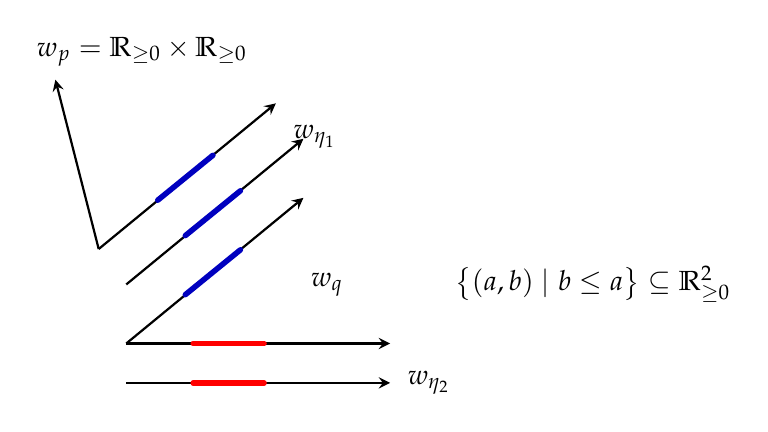
\begin{tikzpicture}[
        x=1cm,
        y=1cm,
        cone ray/.style={thick,->,>=stealth},
        common face/.style={red,line width=2pt,line cap=round},
        diagonal face/.style={blue!75!black,line width=2pt,line cap=round}
    ]
        % The cone at the marked point.
        \coordinate (p) at (0,4.45);
        \draw[cone ray] (p) -- ++(-0.55,2.15);
        \draw[cone ray] (p) -- ++(2.25,1.85);
        \draw[diagonal face]
            ($(p)+(0.75,0.62)$) -- ($(p)+(1.45,1.19)$);
        \node[above] at ($(p)+(0.55,2.2)$)
            {$w_p=\R_{\geq 0}\times\R_{\geq 0}$};

        % The cone at the first generic point.
        \coordinate (etaone) at (0.35,4);
        \draw[cone ray] (etaone) -- ++(2.25,1.85);
        \draw[diagonal face]
            ($(etaone)+(0.75,0.62)$) -- ($(etaone)+(1.45,1.19)$);
        \node[above right] at ($(etaone)+(2.0,1.6)$) {$w_{\eta_1}$};

        % The cone at the node.
        \coordinate (q) at (0.35,3.25);
        \draw[cone ray] (q) -- ++(2.25,1.85);
        \draw[cone ray] (q) -- ++(3.35,0);
        \draw[diagonal face]
            ($(q)+(0.75,0.62)$) -- ($(q)+(1.45,1.19)$);
        \draw[common face] ($(q)+(0.85,0)$) -- ($(q)+(1.75,0)$);
        \node at ($(q)+(2.55,0.75)$) {$w_q$};
        \node[anchor=west] at ($(q)+(4.05,0.75)$)
            {$\bigl\{(a,b)\mid b\leq a\bigr\}\subseteq\R_{\geq 0}^{2}$};

        % The colored intervals indicate the common faces used in the gluing.
        \coordinate (etatwo) at (0.35,2.75);
        \draw[cone ray] (etatwo) -- ++(3.35,0);
        \draw[common face] ($(etatwo)+(0.85,0)$) -- ($(etatwo)+(1.75,0)$);
        \node[right] at ($(etatwo)+(3.45,0)$) {$w_{\eta_2}$};
    \end{tikzpicture}
\end{figure}


\subsection{Tropical curves}%
\label{sub:Tropical curves}

\begin{defn}
    A family of \textit{tropical curves} \((G, \vec{g}, \vec{\ell})\) over a cone \(w, N_w\) consists of
    \begin{enumerate}
        \item A connected graph \(G = V(G) \cup E(G) \cup L(G)\);
        \item A leg ordering \(\vec{m} \colon L(G) \xrightarrow{\sim} \ab\{1, \ldots, n\}\);
        \item A genus function \(\vec{g} \colon V(G) \to \N\);
        \item An edge length function \(\ell \colon E(G) \to \Hom(w \cap N_w, \N) \setminus \ab\{0\}\).
    \end{enumerate}
\end{defn}

Now we will construct \(\Sigma(G, \ell)\). For \(v \in V(G)\), we set \(w_v = w\). For \(e \in E(G)\), we set
\[ w_e = \ab\{ (s, \lambda) \mid \lambda \leq \vec{\ell}(e)(s) \} \subseteq w \times \R_{\geq 0}. \]
For legs \(\ell \in L(G)\), we set \(w_{\ell} = w \times \R_{\geq 0}\). We now need to define the face maps. If \(\ell\) is incident to \(v\), then the face map is
\[ w_v \hookrightarrow w_{\ell} \mid w \mapsto (s, 0). \]
If \(e\) is incident to two vertices \(v_1, v_2\), then the face maps are
\begin{align*}
    w_{v_1} \hookrightarrow w_e &\colon s \mapsto (s, \vec{\ell}(e)(s)) \\
    w_{v_2} \hookrightarrow w_e & \colon s \mapsto (s, 0).
\end{align*}
\begin{rmk}
    The choice of \(v_1\) and \(v_2\) does not change the cone complex up to isomorphism, but it does matter when we want to define contact orders for log maps. However, in general there is no canonical way to make this choice.
\end{rmk}

\subsection{Punctured curves}%
\label{sub:Punctured curves}

We consider a nodal curve
\[ \Spec k[x,y]/xy \to \Spec k \]
with log structures given by \(\N^2\) with chart \((a,b) \mapsto x^a y^b\) and \(\N \to k\) being the standard log point. Now consider \(\ul{C}_1 = Z(x) = \Spec k[y]\) and mark the node by \(p \colon \Spec k \to \Spec k[y]\). Note that
\[ C^{\on{can}} = (\ul{C}, M_C) \to S^{\on{can}} = \Spec(\N \to k). \]
Denote \(M_{C_1}^{\circ} = M_C|_{C_1}\). Then we see that on log structures we have the diagram
\begin{equation*}
\begin{tikzcd}
    k[y] & & \N^2 \ar{ll}[swap]{(a,b) \mapsto 0^a y^b} \\
    k \ar{u} & & \N \ar{ll} \ar{u}{\Delta}.
\end{tikzcd}
\end{equation*}
In particular, we can compute the stalk \(\bar{M}_{C_1}^{\circ}|_p = \N^2\), and therefore we have
\[ \bar{\pi}_{C_1^{\circ}}^{\flat} |_p \colon \N \xrightarrow{\Delta} \N^2. \]
However, we should have the map
\[ \bar{\pi}^{\flat}_{C_1}|_p \colon \N \xrightarrow{i_1} \N \oplus \N, \]
and therefore \(C_1\) is \textbf{not} a log curve. We can then consider the diagram
\begin{equation*}
\begin{tikzcd}
    \N \oplus \Z \\
    \N^2 \ar[hookrightarrow]{u} \ar{rr}{(0,1)\mapsto (0,1)}[swap]{(1,0)\mapsto (1,1)} & & \N^2 \ar{ull}[swap]{\Vectorstack{{(1,0)\mapsto(1,-1)} {(0,1)\mapsto(0,1)}}} \\
    & \N \ar{ul}{i_1} \ar{ur}{\Delta}.
\end{tikzcd}
\end{equation*}
Therefore, we will consider extending the log structures.

Recall that for a log curve, we have \(M_{\mc{C}} = M_{\mc{C}}' \oplus_{\mc{O}_{\mc{C}}^{\times}} P_{\mc{C}}\), where \(P_{\mc{C}}\) is the divisorial log structure by the markings.

\begin{defn}
    A \textit{punctured curve} over an fs log scheme \(S\) consists of \((\mc{C}^{\circ} \xrightarrow{p} \mc{C} \xrightarrow{\pi} S, \{p_i\}_{i=1}^n)\), where \((\mc{C} \xrightarrow{\pi} S, \vec{p})\) is a log curve and the map \(p \colon \mc{C}^{\circ} \to \mc{C}\) is a map of fine log schemes satisfying the following conditions:
    \begin{enumerate}
        \item The underlying map \(\ul{p}\) is an isomorphism;
        \item On log structures, the map \(p^{\flat} \colon M_{\mc{C}} \hookrightarrow M_{\mc{C}^{\circ}}\) is an isomorphism away from the \(p_i\) and induces
            \[ M_{\mc{C}} \xrightarrow{p^{\flat}} M_{C^{\circ}} \hookrightarrow M_{\mc{C}} \oplus P^{\mr{gp}}. \]
        \item For any marking \(p_i\) and any \(s \in M_{\mc{C}^{\circ}, p_i} \setminus M_{\mc{C}, p_i}\), we have \(\alpha_{\mc{C}^{\circ}}(s) = 0\).
    \end{enumerate}
\end{defn}

Roughly speaking, a punctured curve is a log curve plus the data of a commutative diagram
\begin{equation*}
\begin{tikzcd}
    M_{\mc{C}^{\circ}} \ar{dr} \ar[hookrightarrow]{r} & M_{\mc{C}}' \oplus_{\mc{O}_{\mc{C}}^{\times}} P^{\on{gp}} \\
    & \mc{O}_{\mc{C}} \\
    \mc{M}_{\mc{C}} \ar[hookrightarrow]{uu} \ar{ur}.
\end{tikzcd}
\end{equation*}


\begin{exm}
    Let \((\ul{\mc{C}} \to \ul{S} = \Spec k, p)\) be a smooth \(1\)-pointed curve.
    \begin{enumerate}
        \item Let \((\mc{C}/S, p)\) be endowed with the canonical log structure (so \(S\) has no log structure). Let \(M_{\mc{C}} = P\). Then any puncturing \(p^{\flat} \colon M_{\mc{C}} \hookrightarrow M_{\mc{C}^{\circ}} \subset P^{\on{gp}}\) must be trivial. The reason is that \(M_{\mc{C}^{\circ}}\) cannot have a section \(s\) such that \(\alpha_{\mc{C}^{\circ}} = 0\). If \(S \in P = M_{\mc{C}}\), then \(\alpha_{\mc{C}^{\circ}}(s) = \alpha_{\mc{C}}(s)\). Otherwise, if \(s \notin P\), then because \(\alpha_{\mc{C}^{\circ}}(-s)\) is nonzero, so is \(\alpha_{\mc{C}^{\circ}}(s)\).
        \item Let \(M_{\mc{C}^{\circ}} \subseteq (\N \oplus \mc{O}_{\mc{C}}^{\times}) \oplus P^{\on{gp}}\) be a puncturing. Choose a local generator \(x\)  of \(\mc{O}(-p)\). Then any \(s \in M_{\mc{C}^{\circ}, p}\) has the form \(s = ((n, \varphi), x^m)\) where \(n \in \N\) and \(\varphi \in \mc{O}_{\mc{C}, p}^{\times}\). If \(m < 0\), then we require that \(\alpha_{\mc{C}^{\circ}}(s) = 0\). This implies that \(\alpha_{\mc{C}}((n, \varphi), 0) = 0\), and therefore
            \[ \bar{M}_{\mc{C}^{\circ}, p} \subseteq \ab\{(n, m) \in \N \oplus \Z \mid m \geq 0 \text{ if } n = 0 \}. \]
            In fact, any fine submonoid of the right hand side containing \(\N \oplus \N\) can be realized by a puncturing.
        \item Let \(S = \Spec(\N \to k)\). Consider \(M_{\mc{C}^{\circ}}\) such that \(\bar{M}_{\mc{C}^{\circ}, p} = \N^2 + \N (2,-2)\). Because \((1,-1) \notin \bar{M}_{\mc{C}^{\circ}, p}\), we see that \(M_{\mc{C}^{\circ}}\) is not saturated.
    \end{enumerate}
\end{exm}

\begin{lem}
    Let \(Q\) be a sharp fs monoid. Let \(w \coloneqq \Hom(Q, \R_{\geq 0}) = \Q_{\R}^{\vee}\). Let \(Q^{\circ} \subseteq Q \oplus \Z\) be finitely generated with \(Q \oplus \N \subsetneq Q^{\circ}\) and \(Q^{\circ} \cap \ab\{0\} \times \Z_{<0} = \emptyset\). Then there exists a nonzero, concave, piecewise linear function
    \[ \ell \colon w \to \R_{\geq 0} \]
    with rational slopes such that
    \[ (Q^{\circ})_{\R}^{\vee} = \ab\{ (s, \lambda) \in w \times \R_{\geq 0} \mid 0 \leq \lambda \leq \ell(s) \}. \]
\end{lem}

\begin{exm}
    Let \(Q = \N^2\) and set 
    \begin{align*}
        Q^{\circ} &= \ab<((1,0), -1), ((0,1), -1), ((0,0),1)> \subset \N^2 \oplus \Z \\
        &= \ab\{((a,b), m) \mid a+b+m \geq 0, a,b \geq 0 \}.
    \end{align*}
    Then
    \[ (Q^{\circ})_{\R}^{\vee} = \ab\{ (e_x, e_y, e_t) \mid 0 \leq e_t \leq \min(e_x, e_y) \}. \]
\end{exm}





\section{Intro to GW theory with a view to higher genus (Patrick Lei)}%
\label{sec:Intro to GW theory with a view to higher genus (Patrick Lei)}


\subsection{Introduction to GW theory}%
\label{sub:Introduction to GW theory}

The goal of these lectures is to discuss Gromov-Witten theory in a way that is amenable to doing calculations in higher genus. Gromov-Witten theory concerns itself with integrals on the moduli space \(\Mbar_{g,n}(X, \beta)\), where \(X\) is a smooth projective algebraic variety and \(\beta \in H_2(X, \Z)\) is an effective curve class. There is a diagram
\begin{equation*}
\begin{tikzcd}
    \mc{C} \ar{r}{f} \ar[bend right=20]{d}[swap]{\pi} & X \\
    \Mbar_{g,n}(X, \beta) \ar[bend right=20]{u}[swap]{\sigma_i} \ar{ur}[swap]{\on{ev}_i}
\end{tikzcd}
\end{equation*}
where \(\mc{C}\) is the universal curve, \(\sigma_i\) are the sections of \(\pi\) which give the marked points, \(f\) is the universal stable map, and \(\ev_i = f \circ \sigma_i\) are evaluation morphisms. While \(\Mbar_{g,n}(X, \beta)\) is generally singular, not equidimensional, and reducible, there is a special class
\[ [\Mbar_{g,n}(X, \beta)]^{\vir} \in A_{\ab(c_1(X), \beta) + (\dim X - 3)(1-g) + n}(\Mbar_{g,n}(X, \beta), \Q), \]
which is known as the \textit{virtual fundamental class}. 

\begin{exer}
    Use standard arguments in deformation theory to verify that the ``expected dimension'' of \(\Mbar_{g,n}(X, \beta)\) the number given above.
\end{exer}

Under the assumption that \(X\) is smooth and projective, \(\Mbar_{g,n}(X, \beta)\) is proper, so we may define \textit{GW invariants}
\[ \ab<\tau_{a_1}(\alpha_1), \cdots, \tau_{a_n}(\alpha_n)>_{g,n,\beta} \coloneqq \ab(\prod_{i=1}^n \ev_i^* \alpha_i \cdot \psi_i^{a_i}) \cap [\Mbar_{g,n}(X, \beta)]^{\vir} \]
for \(\alpha_i \in H^*(X)\). Here, the \(\psi_i\) are defined by \(\psi_i = c_1(\sigma_i^*(\omega_{\pi}))\).

Unfortunately, calculating individual Gromov-Witten invariants is very difficult, so we will consider the even more difficult problem of studying generating series of GW invariants, for example
\[ F_g = \sum_{\beta \geq 0} q^{\beta} \ab<>_{g,0,\beta} \]
when \(X\) is a Calabi-Yau threefold. Here, \(q\) is a formal variable which keeps track of the curve class and we will denote the ring \(\Q\ps{q^{\beta} \mid \beta \in H_2(X, \Z)_{\mr{eff}}}\) by \(\Lambda\). There are some other structures we will consider. First, we may consider the \textit{quantum cohomology ring}, whose product \(a \star_{\mbf{t}} b\) is given by the formula 
\[
    (a \star_{\mbf{t}} b, c) = \sum_{\substack{\beta \geq 0 \\ n \geq 0}} \ab<a,b,c, \mbf{t}, \ldots, \mbf{t}>_{0,3+n,\beta} \frac{q^{\beta}}{n!}.
\]
Here \(a,b,c, \mbf{t} \in H^*(X)\). We will also consider the \textit{quantum connection}. Let \(\ab\{ e_i \}\) be a basis for \(H^*(X)\). Then the quantum connection is the connection on the trivial bundle with fiber \(H^*(X)\) over \(H^*(X) \times \P^1_z\) given by the formula
\[ \nabla_{t^i} = \partial_{t^i} + \frac{1}{z} e_i \star_{\mbf{t}}. \]
Sometimes, it is useful to also consider the connection in the \(z\)-direction given by 
\[ \nabla_{z \odv{}{z}} \coloneqq z \odv{}{z} - \frac{1}{z} E_X \star_{\mbf{t}} + \mu_X, \]
where \(\mu_X(\alpha) = \frac{\deg(\alpha) - \dim X}{2} \alpha\) is the grading operator and
\[ E_X = c_1(X) + \sum_i \ab(1 - \frac{\deg(e_i)}{2})t^i e_i \]
is the \textit{Euler vector field}. Because we will be mostly interested in Calabi-Yau varieties, we will not consider this.

\subsection{Enumerative mirror symmetry in genus zero}%
\label{sub:Enumerative mirror symmetry in genus zero}

The impetus for mathematicians to develop and study Gromov-Witten theory came in the early 1990s, when a group of physicists predicted the number of rational curves of low degree on a general quintic threefold by converting the problem to one of computing period integrals on a different Calabi-Yau threefold called the \textit{mirror quintic} (equivalently, studying its variation of Hodge structure). In genus zero, all invariants can be recovered from the \textit{J-function} \(J_{\mbf{t}}(q,z) \in H^*(X, \Lambda)[z]\), which is defined by
\[ \ab( J_{\mbf{t}}(q, z), \alpha ) \coloneqq (z + \mbf{t}, \alpha) + \sum_{n, \beta} \frac{q^{\beta}}{n!} \ab< \frac{\alpha}{z-\psi}, \mbf{t}, \ldots, \mbf{t}>_{0,1+n, \beta} \]
for any \(\mbf{t} \in H^*(X, \Lambda)[z]\)  \(\alpha \in H^*(X)\), where \((-,-)\) is the Poincar\'e pairing. Therefore, the problem of computing all genus-zero Gromov-Witten invariants with descendants (these are the \(\psi\)-classes) reduces to the problem of computing the J-function.

\begin{rmk}
    We expand \(\frac{1}{z-\psi}\) as \(\sum_{k=0}^{\infty} \psi^k z^{-k-1}\).  
\end{rmk}

We should note that the J-function can be obtained via a fundamental solution to the quantum differential equation, which is given by
\[ ( S_{\mbf{t}}(z) \phi , \alpha) = (\phi, \alpha) + \sum_{n, \beta} \frac{q^{\beta}}{n!} \ab<\frac{\alpha}{z-\psi}, \phi, \mbf{t}, \ldots, \mbf{t}>_{0, 2+n, \beta}. \]
This has the property that \(S_{\mbf{t}}^*(-z) S_{\mbf{t}}(z) = \on{Id}\), which is usually known as the \textit{symplectic property}. From this, we can recover the J-function by \(z S_{\mbf{t}}^*(z)\cdot 1 = J_{\mbf{t}}(q, z)\).

In physics, mirror symmetry is a duality between two different theories called the A-model and B-model, so now we will need to introduce the B-model object. In the interest of time (and notation), we will assume that \(X\) is a toric variety and that \(-K_X\) is nef. Let \(D_1, \ldots, D_r\) be the complete set of torus-invariant divisors in \(X\). Then define the \(I\)-function
\[
    I_{\mbf{t}}(q, z) \coloneqq z e^{\mbf{t}/z} \sum_{\beta \geq 0} q^{\beta} \frac{\prod_{i=1}^r \prod_{m = -\infty}^{0} (D_i + mz)}{\prod_{i=1}^r \prod_{m=-\infty}^{\beta \cdot D_j} (D_i + mz)}.
\]
Note here that we expand any \((D_i + mz)^{-1}\) which appears as \(\frac{1}{mz} \ab(1 - \frac{D_i}{mz} + \cdots)\), or namely, as a geometric series in \(\frac{D_i}{mz}\). In addition, the I-function is annihilated by a differential equation known as the \textit{Picard-Fuchs equation}, which is some hypergeometric type equation.

\begin{exm}
    If \(\mbf{t} = 0\) and \(X = \P^1\), we obtain
    \begin{align*}
        I(q,z) &= z\sum_{d \geq 0} q^d \frac{1}{\prod_{m=0}^d (H + mz)^2} \\
        &= z\sum_{d \geq 0} \ab(\frac{q}{z^2})^d \frac{1}{(d!^2)} + O(H),
    \end{align*}
    so in fact we see the Bessel function of the first kind as the leading term.
\end{exm}

If \(X\) is a complete intersection in a toric variety \(Y\) cut out by line bundles \(L_1, \ldots, L_k\), all of which satisfy \(H^1(f^* L_i) = 0\) for any genus zero stable map to \(Y\) (this is called being \textit{convex}), then the quantum Lefschetz theorem allows us to replace \([\Mbar_{g,n}(X, \beta)]^{\vir}\) with \(e\ab(\bigoplus \pi_* f^* L_i) \cap [\Mbar_{g,n}(Y, \beta)]^{\vir}\) and perform all computations on \(Y\). In this case, the I-function is defined to be
\[
    I_{\mbf{t}}(q,z) \coloneqq z e^{\mbf{t}/z} \sum_{\beta \geq 0} q^{\beta} \frac{\prod_{i=1}^k \prod_{m=-\infty}^{L_i \cdot \beta} (L_i + mz)}{\prod_{i=1}^k \prod_{m=-\infty}^{0} (L_i + mz)} \frac{\prod_{i=1}^r \prod_{m = -\infty}^{0} (D_i + mz)}{\prod_{i=1}^r \prod_{m=-\infty}^{\beta \cdot D_j} (D_i + mz)},
\]
where we abuse notation and conflate the \(L_i\) with their first Chern classes.

\begin{exm}
    For the quintic threefold, which is cut out by a section of \(\mc{O}_{\P^4}(5)\)  the I-function at \(\mbf{t} = 0\) is given by
    \[ I(q,z) = z \sum_{d \geq 0} q^d \frac{\prod_{m=1}^{5d}(5H+mz)}{\prod_{m=1}^d (H+mz)^5}. \]
\end{exm}

The content of the genus zero mirror theorem is a correspondence between these two objects. More precisely, in the case where \(-K_X\) is nef, they are related by a change of variables.

\begin{thm}
    Write the I-function with \(\mbf{t} = 0\) as \(I_0(q) \cdot z + I_1(q) + O(z^{-1})\). Then we have 
    \[
        J_{\tau(\mbf{t})}(q,z) = \frac{I_{\mbf{t}}(q,z)}{I_0(q)},
    \]
    where \(\tau(\mbf{t}) = \frac{\mbf{t} + I_1(q)}{I_0(q)}\). 
\end{thm}

\begin{exm}
    When \(X = \P^1\), note that \(I_0(q) = 0\) and \(I_1(q) = 0\), so in fact, we have the equality
    \[ J_{\mbf{t}}(q,z) = I_{\mbf{t}}(q,z). \]
\end{exm}

\begin{exm}
    When \(X\) is the quintic threefold, we will rewrite the components of the I-function as \(I_0(q) \cdot z + I_1(q)H + O(z^{-1})\) for convenience. We have
    \[ I_0(q) = \sum_{d \geq 0} \frac{(5d)!}{(d!)^5} q^d, \qquad I_1(q) = H \sum_{d \geq 0} \frac{(5d)!}{(d!)^5} \ab(5\sum_{m=d+1}^{5d} \frac{1}{m}), \]
    so there is a nontrivial mirror map in this case. Specializing to \(\mbf{t} = 0\), we see that \(\tau = \frac{I_1(q)H}{I_0(q)}\), so we obtain
    \[ J_{\tau}(q,z) = \frac{I(q,z)}{I_0(q)}. \]
    By the divisor equation, the left hand side also equals \(J(qe^{I_1/I_0}, z)\), and we will also refer to this as the mirror map.  
    Therefore, we can use the mirror theorem to compute $\star_{\tau}$. The quantum connection in the direction of \(H^2\) becomes the ODE
    \[ (H+zD) S_{\tau}(z)^* = S_{\tau}(z)^* \cdot I_{11} H \star_{\tau}, \]
    where $D \coloneqq q \odv{}{q}$ (here, the coordinate is $\log q$) and $I_{11} \coloneqq 1 + D \ab(\frac{I_1(q)}{I_0(q)})$. An explicit computation using the mirror theorem and the results of Zagier-Zinger yields
    \begin{align*}
        I_{11} H + \cdots &= S_{\tau}(z)^* (I_{11} H \star_{\tau} \1) \\
        \ab( 1 + D\ab(\frac{\frac{I_1}{I_0} + D \ab(\frac{I_2}{I_0})}{I_{11}}) ) H^2 + \cdots &= S_{\tau}(z)^* (I_{11} H \star_{\tau} H) \\
        I_{11} H^3 &= S_{\tau}(z)^* (I_{11}H \star_{\tau} H^2).
    \end{align*}
    Because $S_{\tau}$ begins with the identity, this computes $H \star_{\tau}$.
\end{exm}

\subsubsection{Oscillating integrals}%
\label{ssub:Oscillating integrals}

We will now reinterpret the genus zero mirror theorem, and we will return to this interpretation when we discuss higher genus invariants. In particular, we will interpret the I-function as an integral on some mirror family to \(X\), which for us will be a toric variety. Let
\[ 0 \to \Lambda \to \Z^r \to N \to 0 \]
be the fan sequence of \(X\). Applying \(\Hom(-, \C^{\times})\), we obtain the exact sequence
\[ 1 \to (\C^{\times})^{\dim X} \to (\C^{\times})^r \to \Hom(\Lambda, \C^{\times}) \to 1. \]
Suppose that the map \(\Lambda \to \Z^r\) is given by the matrix \((m_{ij})_{i=1,\ldots,r}^{j = 1, \ldots, \rho(X)}\). Then we consider the variety
\[ E_q = \ab(\prod_{i=1}^r x_j^{m_{ij}} = q_i \middle\vert i=1, \ldots, \rho(X)) \]
which is mirror to \(X\) and consider the superpotential \(f = x_1 + \cdots + x_r\). If we wish to consider the equivariant theory with equivariant parameters \(\lambda_1, \ldots, \lambda_r\) acting on each homogeneous coordinate of \(X\), we will consider \(f_{\lambda} = \sum_{i=1}^r (x_i - \lambda_i \log x_i)\). 

\begin{exm}
    When \(X = \P^n\), the mirror to \(X\) is the superpotential \(\sum_{i=1}^{n+1} (x_i - \lambda_i \log x_i)\) on the variety \(E_q = (x_1 \cdots x_{n+1} = q)\).   
\end{exm}

We now choose an appropriate Lefschetz thimble \(\Gamma_{\alpha}\) near each critical point \((x_{\alpha})\) of the (equivariant) superpotential and consider the integral
\[ I_{\alpha} = \int_{\Gamma_{\alpha}} e^{f_{\lambda}/z} \prod_{i=1}^r \frac{\d{x_i}}{x_i}. \]
This corresponds in the I-function to replacing each \(D_i\) in the expression by \(D_i - \lambda_i\) (turning on the equivariant parameters) and in the J-function to considering the fully equivariant GW theory of \(X\). In genus zero, the limit as \(\lambda_i \to 0\) exists, so we can safely recover the original mirror theorem from the following:

\begin{thm}
    This integral is annihilated by the same Picard-Fuchs equation as the I-function, and up to various prefactors, its asymptotic expansion as \(z \to 0^-\) along the negative real axis coincides with the restriction of the I-function corresponding to the T-fixed point on \(X\) which corresponds to the critical point \(( x_{\alpha} )\). 
\end{thm}


\subsubsection{The Lagrangian cone}%
\label{ssub:The Lagrangian cone}

The quantum cohomology of \(X\) is an example of a \textit{Frobenius manifold}, which we will see later can be produced from any cohomological field theory. Write \(V = H^*(X)\) and let \((e_{\mu})\) be a basis for \(V\), so we can write $\bv = \sum_{\mu,n} t^{\mu}_n e_{\mu} z^n \in V\ps{z}$.
The structure of a Frobenius manifold comes from the function
\[
    \mc{F}_0(\bv) = \sum_{n, \beta, \mu} \frac{q^{\beta}}{n!} \ab<\bv(\psi), \ldots, \bv(\psi)>_{0,n,\beta},
\]
which is also called the \textit{genus zero descendant potential} of \(X\). It satisfies the string equation, dilaton equation, and topological recursion relations: 
\begin{align*}
    \pdv{}{t_0^1} \mc{F}_0 &= \frac{1}{2} (\bv_0, \bv_0) + \sum_{n=0}^{\infty} \sum_{\mu} t_{n+1}^{\mu} \pdv{}{t_n^{\mu}} \mc{F}_0; \\
    \pdv{}{t_1^1} \mc{F}_0 &= \sum_{n=0}^{\infty} \sum_{\mu} t_n^{\mu} \pdv{}{t_n^{\mu}}\mc{F}_0 - 2 \mc{F}_0; \\
    \pdv{}{t_{k+1}^{\alpha},t_m^{\beta},t_n^{\gamma}} \mc{F}_0 &= \sum_{\mu,\nu} \pdv{}{t_k^{\alpha},t_0^{\mu}} \mc{F}_0 \cdot \eta^{\mu\nu} \cdot \pdv{}{t_0^{\nu},t_{m}^{\beta},t_n^{\gamma}} \mc{F}_0.
\end{align*}
To state the following result, we consider the infinite-dimensional vector space $V\ls{z^{-1}}$ (or a completion of this) with the symplectic form
\[ \omega(\mbf{f}(z), \mbf{g}(z)) \coloneqq \on{Res}_{z=0}(\mbf{f}(-z), \mbf{g}(z)). \]
We also consider the new variable\footnote{This is called the \textit{dilaton shift}.} $\bq = \bv - z$, so $\mc{F}_0$ is now a function near $\bq = -z$.

\begin{thm}[Givental]
    $\mc{F}$ satisfies the above PDEs if and only if the graph $\mc{L}$ of $\d{\mc{F}}$ is a Lagrangian cone with vertex at $\bq = 0$ such that its tangent spaces $L$ are tangent to $\mc{L}$ exactly along $zL \subset L$.
\end{thm}

We may recover the Lagrangian cone $\mc{L}$ by the following procedure. We find a fundamental solution 
\[ S = \mr{Id} + S_1 z^{-1} + S_2 z^{-2} + \cdots \]
to the quantum connection, which satisfies the equation
\[ z \pdv{}{t^{\mu}}S = e_{\mu} \star S. \]
Then, setting $J \coloneqq z S^*(z) \1$, we can then recover the Lagrangian cone by the following procedure:
\begin{itemize}
    \item The derivatives $\pdv{}{t^{\mu}} J$ form a basis of $L \cap V\ps{z^{-1}}$;
    \item This implies that $z \pdv{}{t^{\mu},t^{\nu}} \in L \cap V \ps{z^{-1}}$. Writing these in terms of the first derivatives and using the fact that $J$ solves the quantum connection, we recover the Frobenius structure and hence the Lagrangian cone.
\end{itemize}

Using this, we can interpret the genus zero mirror theorem as:
\begin{thm}
    The I-function \(I_{\mbf{t}}(q,z)\) lies on the Lagrangian cone of \(X\).
\end{thm}




\subsection{Moduli of curves and CohFTs}%
\label{sub:Moduli of curves and CohFTs}

We will denote by $\Mbar_{g,n}$ the moduli space of stable curves of genus $g$ with $n$ marked points. This is nonempty if and only if $2g-2+n > 0$, in which case it is a Deligne-Mumford stack of dimension $3g-3+n$. There is a combinatorial structure to the collection of $\Mbar_{g,n}$, which is given by a collection of morphisms.
\begin{itemize}
    \item There is the gluing morphism 
        \[q \colon \Mbar_{g,n+1} \times \Mbar_{h, m+1} \to \Mbar_{g+h,n+m}, \] 
        which takes two curves and glues them along the last marked point to form a node;
    \item There is the self-gluing morphism \[s \colon \Mbar_{g-1,n+2} \to \Mbar_{g,n},\] 
        which glues the last two marked points.
\end{itemize}
There is of course another interesting map, which is the forgetful map
\[ \pr \colon \Mbar_{g,n+1} \to \Mbar_{g,n} \]
given by deleting the last marked point and then stabilizing. We are now able to define our enumerative theories of interest, which include Gromov-Witten theory.

\begin{defn}
    Given a vector space $V$ with a nondegenerate symmetric bilinear form $\eta$ and a unit element $\1 \in V$, a \textit{Cohomological Field Theory (CohFT)} $\Omega$ on $V$ is a collection $\Omega_{g,n}$ of $S_n$-equivariant linear maps
    \[ \Omega_{g,n} \colon V^{\otimes n} \to H^*(\Mbar_{g,n}) \]
    which satisfy the basic identity
    \[ \Omega_{0,3}(\1, u,v) = \eta(u,v) \]
    and the following combinatorial identities (we will let $e_{\mu}$ be a basis of $V$ such that $e_1 = \1$ and $e^{\mu}$ be the dual basis):
    \begin{align*}
        q^* \Omega_{g+h,n+m}(\bv_1, \bv_2) &= \sum_{\mu} \Omega_{g,n+1}(\bv_1, e_{\mu}) \cdot \Omega_{h,m+1}(  \bv_2, e^{\mu} ); \\
        s^* \Omega_{g,n}(\bv) &= \sum_{\mu} \Omega_{g,n+2}(\bv, e_{\mu}, e^{\mu}).
    \end{align*}
    If in addition the identity
    \[ \pr^*\Omega_{g,n}(\bv) = \Omega_{g,n+1}(\bv,\1) \]
    is satisfied, then we say the CohFT has a \textit{flat unit} (or satisfies the \textit{string equation}).
\end{defn}
All of this can be generalized to super vector spaces, but for simplicity we will not deal with this case.

\begin{exm}
    The most important example of a CohFT is the Gromov-Witten theory of a smooth projective variety $X$. Here, recall that the source of a stable map is a \textbf{prestable} curve, so there is a stabilization morphism
    \[ \st \colon \Mbar_{g,n}(X,\beta) \to \Mbar_{g,n} \]
    which forgets the map and stabilizes the curve. Then, working over the Novikov ring, we will set $V = H^*(X)$, $\eta$ to be the Poincar\'e pairing, and $\1$ to be the fundamental class of $X$. The linear maps $\Omega^X_{g,n}$ are given by the formulae
    \[ \Omega_{g,n}^X(\btau) \coloneqq \sum_{\beta} q^{\beta} \st_* \ab(\prod_{i=1}^n \ev_i(\tau_i) \cap [\Mbar_{g,n}(X,\beta)]^{\vir}), \]
    where $\ev_i \colon \Mbar_{g,n}(X,\beta) \to X$ is the $i$-th evaluation map.
\end{exm}

\begin{exm}
    Let $\pi \colon \mc{C}_{g,n} \to \Mbar_{g,n}$ be the universal curve. Then the \textit{Hodge bundle} is the vector bundle 
    \[ \E_{g,n} \coloneqq \pi_* \omega_{\pi}. \]
    We then consider the vector space $V = \C$ with the usual pairing and define the CohFT $\Omega^{\E}$ by the formula
    \[ \Omega^{\E}_{g,n} \coloneqq c(\E_{g,n}). \]
    The gluing axioms are satisfied by the equation $q^* \E_{g+h} = \E_g \oplus \E_h$ and the exact sequence
    \[ 0 \to \E_{g-1} \to \E_g \to \mc{O} \to 0. \]
    Here, because genus zero components do not contribute to global sections of $\omega$ and $\E$ does not depend on the marked points, this CohFT has a flat unit.
\end{exm}

\begin{rmk}
    We will see later that this is related to the GW CohFT of a point by the quantum Riemann-Roch theorem. 
\end{rmk}

Given a CohFT $\Omega$, we may produce invariants by pairing the classes $\Omega_{g,n}(\bv)$ with various cohomology classes on $\Mbar_{g,n}$. The most important ones to consider are the classes
\[ \bar{\psi}_i \coloneqq c_1( s_i^* \omega_{\pi} ), \]
where $s_i \colon \Mbar_{g,n} \to \mc{C}_{g,n}$ is the $i$-th marked point.

\begin{rmk}
    In Gromov-Witten theory, these are called \textit{ancestors}. There are also descendants, which are given by the same formula except using the moduli space $\mf{M}_{g,n}$ of prestable curves instead of $\Mbar_{g,n}$, where we factor the morphism $\st$ defined above as
    \[ \Mbar_{g,n}(X,\beta) \xrightarrow{\text{forget map}} \mf{M}_{g,n} \xrightarrow{\text{stabilize}} \Mbar_{g,n}. \]
    The descendant classes are denoted by $\psi_i$.
\end{rmk}

\begin{exm}
    We will calculate an invariant which will appear in the GW theory of Calabi-Yau threefolds. For any CohFT $\Omega$, consider the invariant
    \[ \ab<\1\bar{\psi}_1>_{1,1}^{\Omega}\coloneqq \int_{\Mbar_{1,1}} \Omega_{1,1}(\1)\bar{\psi}_1. \]
    Using the second gluing equation, the degree zero part of $\Omega_{1,1}(\1)$ is equal to
    \[ \sum_{\mu} \Omega_{g,n+2}(\1, e_{\mu}, e^{\mu}) = \sum_{\mu} \eta(e_{\mu}, e^{\mu}), \]
    which yields the (graded) dimension $\chi(V)$ of $V$ (for example, if \(V = H^*(X)\) for a Calabi-Yau threefold \(X\), this is the topologial Euler characteristic of \(X\)). Therefore, we obtain
    \[ \ab<\1\bar{\psi}_1>_{1,1}^{\Omega} = \frac{\dim V}{24}. \]
\end{exm}

\begin{exm}
    Consider the GW CohFT of a point. This is given by $V = \C$ with the usual pairing and the formula 
    \[ \Omega_{g,n} = 1. \]
    Then we define the invariants
    \[ \ab<\bar{\psi}_1^{a_1} \cdots \bar{\psi}_n^{a_n}>_{g,n} \coloneqq \int_{\Mbar_{g,n}} \Omega_{g,n} \cdot \bar{\psi}_1^{a_1} \cdots \bar{\psi}_n^{a_n}. \]
    \begin{thm}[Kontsevich]
        The function
        \[ \mc{D} \coloneqq \exp \ab(\sum_{g,n} \frac{\hbar^{g-1}}{n!}\sum_{a_1 + \cdots + a_n = n} \ab<\bar{\psi}_1^{a_1} \cdots \bar{\psi}_n^{a_n}>_{g,n} t_{a_1}\cdots t_{a_n}) \]
        is annihilated by the operators
        \begin{align*}
            L_{-1} \coloneqq{}& -\pdv{}{t_0} + \frac{\hbar^{-1}}{2} t_0^2 + \sum_{i=0}^{\infty} t_{i+1} \pdv{}{t_i};\\
            L_0 \coloneqq{}& -\frac{3}{2} \pdv{}{t_1} + \sum_{i=0}^{\infty} \frac{2i+1}{2} t_i \pdv{}{t_i} + \frac{1}{16};\\
            L_n \coloneqq{}& -\frac{(2n+3)!!}{2^{n+1}} \pdv{}{t_{n+1}} + \sum_{i=0}^{\infty} \frac{(2i+2n+1)!!}{(2i-1)!! 2^{n+1}} t_i \pdv{}{t_{i+n}} \\
            &+ \frac{\hbar}{2} \sum_{i=0}^{n-1} \frac{(2i+1) (2i-1) \cdots (2i+1-2n)}{2^{n+1}} \pdv{}{t_i,t_{n-1-i}}.
        \end{align*}
    \end{thm}
\end{exm}

\begin{rmk}
    This result (Virasoro constraints for a point) is equivalent to $\mc{D}$ being a tau-function for the KdV hierarchy and has been generalized by various authors.
\end{rmk}



\subsection{$R$-matrix action}%
\label{sub:R-matrix action}

In the early 2000s, Givental discovered a remarkable property of axiomatic enumerative theories, namely that one can transform CohFTs by the action of matrices $R(z) = R_0 + R_1 z + R_2 z^2 + \cdots \in \Hom(V, V')\ps{z}$ which satisfy the property
\[ R^*(-z) R(z) = \mr{Id}_V. \]
Traditionally, the literature requires that $V = V'$ and $R_0 = \mr{Id}$, but the MSP group has removed this restriction and also allows $\dim V < \dim V'$.

In order to define the action of $R$ on a CohFT $\Omega$ defined on $V$, we need to review some of the combinatorial structure of $\Mbar_{g,n}$. For a curve $C\in \Mbar_{g,n}(\C)$, we may consider the dual graph of $C$, which has vertices, edges, and legs, which are defined as follows:
\begin{itemize}
    \item The vertices correspond to irreducible components of $C$ and are labelled by a non-negative integer, which is the genus;
    \item The edges correspond to nodes of $C$ (in particular, we allow loops);
    \item The legs correspond to marked points.
\end{itemize}
Any graph which appears as the dual graph of a stable curve is called a \textit{stable graph}.

\begin{figure}[htpb]
  \centering
  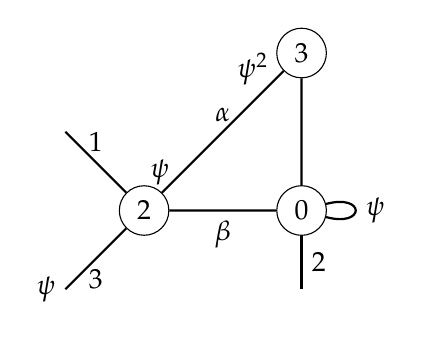
\begin{tikzpicture}[scale=1,transform shape,every loop/.style={}]
    \node[circle,draw] (A) at (0,0) {$2$};
    \node[circle,draw] (B) at (2,2) {$3$};
    \node[circle,draw] (C) at (2,0) {$0$};
    \draw[thick] (A) -- node[above]{$\alpha$} (B) -- (C) -- node[below]{$\beta$} (A);
    \draw[thick] (A) -- node[below]{$3$} (-1,-1);
    \draw[thick] (A) -- node[above]{$1$} (-1,1);
    \draw[thick] (C) -- node[right]{$2$} (2,-1);
    \draw[thick] (C) edge[loop right] node[right] {$\psi$} (C);
    \node[anchor=east] at (-1,-1) {$\psi$};
    \node[anchor=east] at (1.7,1.8) {$\psi^2$};
    \node[anchor=south] at (0.2,0.2) {$\psi$};
  \end{tikzpicture}
  \caption{Example of a stable graph in $\ol{\mc{M}}_{7,3}$ and associated tautological class. This stable graph describes the image of a map
    $\ol{\mc{M}}_{2,4} \times \ol{\mc{M}}_{3,2} \times \ol{\mc{M}}_{0,5} \to \ol{\mc{M}}_{7,3}$.}
  \label{fig:stablegraph}
\end{figure}

The first type of action on CohFTs is a translation action. Let $T \in V\ps{z}$. For a CohFT $\Omega$, we define
\[ (T\Omega)_{g,n}(\bv) \coloneqq \sum_m \frac{1}{m!} p_* \Omega_{g,n+m}(\bv, T,\ldots,T) \]
whenever the infinite sum makes sense.

\begin{exm}
    If $\Omega^X$ is the GW CohFT of a smooth projective variety $X$ and $\tau \in H^2(X)$ is a divisor class, then the infinite sum makes sense and we can define the shifted GW CohFT $\Omega^{X,\tau}$ of $X$. For example, if $X$ is the quintic threefold and $\tau = \frac{I_1}{I_0} H$, then shifting to $\tau$ is the same as the mirror map $q \mapsto Q(q) = q e^{\frac{I_1}{I_0}}$.
\end{exm}

The second type of action is the action of a matrix $R$ as in the beginning of this section. Let $G_{g,n}$ define the set of all stable graphs of genus $g$ with $n$ legs. Then we define
\[ (R\Omega)_{g,n} \coloneqq \sum_{\Gamma \in G_{g,n}} \frac{1}{\ab|\Aut \Gamma|} \on{Cont}_{\Gamma}, \]
where $\on{Cont}_{\Gamma}$ is defined by the following construction:
\begin{itemize}
    \item At the $i$-th leg, we place the map 
        \[ R(-\bar{\psi}_i)^* \in \Hom(V',V) \ps{\bar{\psi}_i}; \]
    \item At every edge, we place the bivector
        \[ V(\bar{\psi}_1, \bar{\psi}_2) \coloneqq \sum_{\mu} \frac{e_{\mu} \otimes e^{\mu} - R(-\bar{\psi}_1)^* e_{\mu} \otimes R(-\bar{\psi}_2)^* e^{\mu}}{\bar{\psi}_1 + \bar{\psi}_2}; \]
    \item At every vertex, we place the linear map
        \[ \Omega_{g_v, n_v} \colon V^{\otimes n_v} \to H^*(\Mbar_{g_v, n_v}); \]
    \item Finally, we consider the pushforward in cohomology along the gluing morphism $\prod_v \Mbar_{g_v, n_v} \to \Mbar_{g,n}$.
\end{itemize}

\begin{defn}
    Let $R$ be as above. Then we define the translation
    \[ T_R \coloneqq z (\1 - R(-z)^* \1') \in z V'\ps{z}. \]
    Whenever it makes sense, we define
    \[ R.\Omega \coloneqq RT\Omega. \]
\end{defn}

\begin{thm}[Chang-Guo-Li]
    Suppose we work with coefficients in $\C\ps{q}$. Then if
    \[ T_R \in z^2 V \ps{z} + zq V \ps{z}, \]
    $R.\Omega$ is a well-defined CohFT. Moreover, if $\dim V = \dim V'$, $\1'$ is a unit for $R.\Omega$.
\end{thm}

We would like to remark a bit more about the translation action when $R_0 \neq \mr{Id}$. For simplicity, we will assume that $V = V'$ and $R_0 \1 = c \cdot \1$ for some constant $c$. Then we set $\tilde{T}_R \coloneqq z( \1 - c R(z)^{-1} \1)$ and use the dilaton equation to compute
\begin{align*}
    T_R \Omega_{g,n}(\bv) &= \sum_{m=0}^{\infty} \frac{1}{m!} p_*\Omega_{g,n+m}(\bv, T_R, \ldots, T_R) \\
    &= \sum_{k,\ell \geq 0} \frac{1}{k!\ell!} p_* \Omega_{g,n+k+\ell}(\bv, ( (1-c^{-1})\1 \cdot \psi )^{\otimes k}, ( c^{-1} \tilde{T}_R )^{\otimes \ell}) \\
    &= \sum_{k,\ell \geq 0} \frac{(1-c^{-1})^k \cdot c^{-\ell}}{\ell!} \binom{2g-2+n+k+\ell-1}{k} p_* \Omega_{g,n+\ell}(\bv, \tilde{T}_R^{\otimes \ell}) \\
    &= \sum_{m=0}^{\infty} \frac{c^{2g-2+n}}{m!} p_* \Omega_{g,n+m}(\bv, \tilde{T}_R, \ldots, \tilde{T}_R)
\end{align*}
whenever this makes sense.


\subsection{Reconstruction theorem}%
\label{sub:Reconstruction theorem}

Recall that every CohFT defines a Frobenius algebra. We will call a CohFT \textit{semisimple} if the corresponding Frobenius algebra is semisimple.

\begin{thm}[Teleman]
    Let $\Omega$ be a semisimple CohFT with flat unit and $\omega$ be its topological part. If $\Omega$ is semisimple, there exists a unique 
    \[ R = \mr{Id} + R_1 z + \cdots \in \End(V)\ps{z} \]
    such that
    \[ \Omega = R.\omega. \]
\end{thm}

\begin{exm}
    Recall the Hodge bundle CohFT from before. Recall that it is given by the formula
    \[ \Omega^{\E}_{g,n} = c(\E) = 1 + \lambda_1 + \cdots + \lambda_g. \]
    Taking the degree zero part, we see that $\omega^{\E}$ is the GW CohFT of a point. Using Mumford's computation
    \[ \ch(\E) = g + \sum_{k=1}^{\infty} \frac{B_{2k}}{(2k)!}\ab(\kappa_{2k-1} + \frac{1}{2}\iota_*\sum_{i=0}^{2k-2} \bar{\psi}_1^{i} \bar{\psi}_2^{2g-2+i}), \]
    where $\kappa_{m} = p_* \bar{\psi}_{n+1}^{m+1}$, $B_{2k}$ are the Bernoulli numbers, and $\iota$ is the inclusion of the boundary up to a $2:1$ \'etale cover, and the formula
    \[ c(E) = \exp \ab(-\sum_k (-1)^k (k-1)!\ch_k(E)) \]
    for any vector bundle $E$ (or by just using the quantum Riemann-Roch theorem\footnote{There is a sign error in Coates-Givental, which has propagated to the rest of the literature.} directly), we obtain the $R$-matrix
    \[ R(z) = \exp\ab( \sum_{k=1}^{\infty} \frac{B_{2k}}{2k(2k-1)} z^{2k-1}) = 1+\frac{1}{12}z + \cdots. \]

    As a sanity check, we will compute $\Omega_{1,1}^{\E}$ using the $R$-matrix. First, we consider the stable graphs in~\Cref{fig:03graphloop}.
    \begin{figure}[htpb]
    \begin{center}
    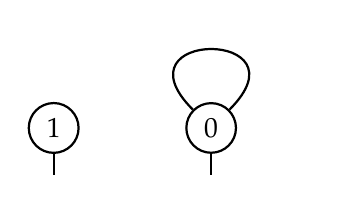
\begin{tikzpicture}[scale=1, transform shape, every loop/.style={}]
    \node[circle,draw=black,thick] (B) at (-1,0) {$1$};
    \draw[-,thick] (B) -- (-1,-0.6);
    \node[circle,draw=black,thick] (A) at (1,0) {$0$};
    \draw[-,thick] (A) -- (1,-0.6);
    \path[every node/.style={font=\sffamily\small},thick]
        (A)   edge[loop] (A);
    \end{tikzpicture}
    \end{center}
    \caption{Stable graphs for $g=1, n=1$}%
    \label{fig:03graphloop}
    \end{figure}
    The first graph $\Gamma_1$ gives us the contribution
    \begin{align*}
        \Cont_{\Gamma_1} &= T\omega_{1,1}^{\E}(R(z)^{-1}\1) \\
        &= \omega_{1,1}^{\E}(R(z)^{-1}\1) + p_* \omega_{1,1}^{\E}(R(z)^{-1}\1, T_R(z)).
    \end{align*}
    Using the formula $B_2 = \frac{1}{6}$ and the fact that $\dim \Mbar_{1,1} = 1$, this becomes
    \[ 1 - \frac{1}{12}\psi_1 + \frac{1}{12} \kappa_1. \]
    The second graph does not receive tail contributions because $\dim \Mbar_{0,3} = 0$. The constant term of the edge contribution is $\frac{1}{12}$, so considering the automorphism and pushing forward to $\Mbar_{1,1}$ gives us
    \[ \Cont_{\Gamma_2} = \frac{1}{12} \Delta, \]
    where $\Delta$ denotes the boundary divisor (with the correct stack structure). Because $\psi_1 = \kappa_1$ in this case, we obtain
    \[ 1+\lambda_1 = 1 + \frac{1}{12}(\kappa_1 - \psi_1 + \Delta) = 1 + \frac{1}{12} \Delta. \]
\end{exm}




\subsection{Operator formalism and geometric quantization}%
\label{sub:Operator formalism and geometric quantization}

We will return to the symplectic formalism of Givental. This is more convenient for certain computations, but it is in fact equal to what we have before, at least when we want to calculate generating functions. Recall that we had a Frobenius manifold structure on $V$ and we considered the vector space $\mc{V}\coloneqq V\ls{z^{-1}}$ with symplectic form
\[ (\mbf{f}(z), \mbf{g}(z)) \coloneqq \on{Res}_{z=0} \eta(\mbf{f}(-z), \mbf{g}(z)). \]
If we consider the polarization given by $\mc{V}_+ = V[z]$ and $\mc{V}_- = z^{-1}V\ps{z^{-1}}$, then letting $\bq$ be as before (with the dilaton shift), let $\bp$ be coordinates on $\mc{V}_-$ such that $(\bq, \bp)$ form a system of Darboux coordinates for $\mc{V}$.

\begin{defn}
    We will call any formal function of the form
    \[ \mc{D} = \exp\ab(\sum_{g=0}^{\infty} \hbar^{g-1} \mc{F}_g) \]
    an \textit{asymptotic element of the Fock space}.
\end{defn}

Then given such an asymptotic element of the Fock space, we will quantize (infinitesimal) symplectic transformations on $\mc{V}$ by the following formulae:
\[ \wh{p_a p_b} \coloneqq \hbar \partial_{q_a} \partial_{q_b}, \qquad \wh{p_a q_b} \coloneqq q_b \partial_{q_a}, \qquad \wh{q_a q_b} = \frac{q_a q_b}{\hbar}. \]
In particular, this will allow us to understand expressions like $\hat{R} \mc{D}$. However, we need to be careful because our formulae will involve both the fundamental solution $S_{\tau}$ and the $R$-matrix, and $S_{\tau}$ is a power series in $z^{-1}$.\footnote{This is because we expand $\frac{1}{z-\psi} = \sum_{n=0}^{\infty} \psi^n z^{-n-1}$.}

\begin{thm}[Givental]
    An operator of the form $S(z^{-1}) = \mr{Id} + S_1 z^{-1} + \cdots$ acts on (asymptotic) elements of the Fock space by the formula
    \[ \hat{S}^{-1} \mc{D}(\bq) = e^{\frac{1}{2\hbar}W(\bq,\bq)} \mc{D}([S \bq]_+), \]
    where $W = \sum \eta(W_{mn}q_m, q_n)$ is defined by the formula
    \[ \frac{S(w^{-1})^* S(z^{-1}) - \mr{Id}}{w^{-1}+z^{-1}} = \sum \frac{W_{mn}}{w^m z^n}. \]
    Operators of the form $R(z) = \mr{Id} + R_1 z + \cdots$ act by the formula
    \[ \hat{R}\mc{D}(\bq) = e^{\frac{\hbar}{2} V(\partial_{\bq}, \partial_{\bq})} \mc{D}(R^{-1} \bq), \]
    where $V = \sum \eta(p_m, V_{mn} p_n)$ is defined by 
    \[ \frac{R(w)^* R(z) - \mr{Id}}{w+z} = \sum V_{mn} w^m z^n. \]
\end{thm}

For a semisimple CohFT, there is a system of \textit{canonical coordinates} $u_{\alpha}$ such that the $1$-form $\d{u}$ is a homomorphism of algebras $T_v V \to \C$. Then near a semisimple point, there is a asymptotic solution to the quantum connection of the form
\[ \Psi \cdot  R \cdot e^{\frac{U}{z}}, \]
where $\Psi$ switches from flat coordinates to canonical coordinates and $U = \on{diag}(u_{\alpha})$ is the matrix of canonical coordinates. Finally, define
\[ C = \frac{1}{2} \int^u \sum R_1^{\alpha\alpha} \d{u_{\alpha}}. \]
A corollary of Teleman's reconstruction theorem is the formula
\[ \mc{D}^X = e^{C(u)} \hat{S}^{-1}_{\tau} \hat{\Psi} \hat{R} \wh{e^{\frac{U}{z}}} \prod_{i=1}^{\dim V} \mc{D}^{\mr{pt}} \]
for the Gromov-Witten theory of any smooth projective variety with semisimple quantum cohomology.

\begin{exm}
    As a final example, we will apply Teleman's theorem to compute $F_1$ of any semisimple CohFT. Let $e_{\mu}$ denote an idempotent basis for the quantum product. We will compute
    \[ \int_{\Mbar_{1,1}} \Omega_{1,1}(e_{\beta}). \]
    Using the reconstruction theorem, we obtain
    \begin{align*}
        \int_{\Mbar_{1,1}}\Omega_{1,1}(e_{\beta}) ={}& \int_{\Mbar_{1,1}} T_R \omega_{1,1}(R(\bar{\psi})^{-1} e_{\beta}) + \frac{1}{2} T_R \omega_{0,3}(R(\bar{\psi})^{-1} e_{\beta}, V(\bar{\psi}_2, \bar{\psi}_3)) \\
        ={}& \int_{\Mbar_{1,1}}T_R\omega_{1,1}(e_{\beta}) - \int_{\Mbar_{1,1}} T_R \omega_{1,1}(R_1 e_{\beta})\bar{\psi} \\ 
        &+ \frac{1}{2}\sum_{\mu}  \omega_{0,3}(e_{\beta}, R_1 e^{\mu}, e_{\mu}) \\
        ={}& \int_{\Mbar_{1,1}} ( \omega_{1,1}(e_{\beta}) + p_* ( \omega_{1,2}(e_{\beta}, R_1 \1) \bar{\psi}_2^2 )) \\
        &- \int_{\Mbar_{1,1}} (\omega_{1,1}(R_1 e_{\beta})\bar{\psi}_1 + p_* ( \omega_{1,2}(R_1 e_{\beta}) \bar{\psi}_2^2 ) \bar{\psi}_1) \\
        &+ \frac{1}{2} \sum_{\mu} \eta(e_{\beta} \star e_{\mu}, R_1 e^{\mu}) \\
        ={}& \frac{1}{24} \sum_{\mu} ( \omega_{0,4}(e_{\mu}, e^{\mu}, e_{\beta}, R_1 \1) -\omega_{0,3}(e_{\mu}, e^{\mu}, R_1 e_{\beta}) )\\
        &+ \frac{1}{2} \eta(e_{\beta}, R_1 e^{\beta}) \\
        ={}& \frac{1}{24} \sum_{\mu}\sum_{\nu} \omega_{0,3}(e_{\mu}, e^{\mu}, e_{\nu})\omega_{0,3}(e^{\nu}, e_{\beta}, R_1 \1) \\
        &-\frac{1}{24} \sum_{\mu} \omega_{0,3}(e_{\mu}, e^{\mu}, R_1 e_{\beta}) + \frac{1}{2} (R_1)_{\beta\beta} \\
        ={}& \frac{1}{24} \ab(\eta(e^{\beta}, R_1 \1) - \sum_{\mu} \eta(e^{\mu}, R_1 e_{\beta})) + \frac{1}{2} (R_1)_{\beta\beta}.
    \end{align*}
    Using the identities
    \begin{align*}
        \eta(R_1 \1, e^{\beta}) - \sum_{\mu} \eta(R_1 e_{\beta}, e^{\mu}) &= \sum_{\mu} \Delta_{\mu} \int_{\Mbar_{0,4}} \Omega_{0,4}(e_{\mu}, e_{\mu}, e_{\mu}, e_{\beta}) \\
        &= -\frac{1}{2}\sum_{\mu} \Delta_{\mu} \partial_{u_{\beta}} \Delta_{\mu}^{-1} \\
        &= \frac{1}{2} \sum_{\mu} \partial_{u_{\beta}} \log \Delta_{\mu},
    \end{align*}
    where $\Delta_{\mu} \coloneqq \eta(e_{\mu}, e_{\mu})^{-1}$, we obtain the result
    \[ \int_{\Mbar_{1,1}} \Omega_{1,1} e_{\beta} = \frac{1}{48} \sum_{\mu} \partial_{u_{\mu}} \log \Delta_{\mu} + \frac{1}{2} (R_1)_{\beta\beta}, \]
    which can be placed in the suggestive form
    \[ \d{F_1^{\Omega}} = \sum_{\mu} \frac{\d{\log \Delta_{\mu}}}{48} + \frac{1}{2} (R_1)_{\mu\mu} \d{u_{\alpha}}. \]
    This recovers a result which was already known to Givental.
\end{exm}

\subsection{How to compute the R-matrix}%
\label{sub:How to compute the R-matrix}

We will conclude by explaining how to compute the R-matrix, starting in the setting where the Frobenius manifold is conformal (for example the Gromov-Witten theory of a smooth projective variety, \(r\)-spin curves, etc). In this example, we will consider the Frobenius manifold for 3-spin curves. Let \(V\) be 2-dimensional with coordinates \(x\) and \(y\), where \(x\) corresponds to the unit. The metric is given by
\[ \eta = \begin{pmatrix}
    0 & 1 \\
    1 & 0
\end{pmatrix} \]
and the primary genus zero potential is \(F(x,y) = \frac{1}{2} x^2 y + \frac{1}{72} y^4\). There is an \textit{Euler vector field}
\[ E = x \pdv{}{x} + \frac{2}{3} y \pdv{}{y}, \]
which acts with weights \(-1\) and \(-\frac{2}{3}\) on \(\partial_x\) and \(\partial_y\), respectively. The conformal dimension is \(\delta = \frac{1}{3}\), and we will define the degree operator
\[ \mu(v) = [E,v] + \ab(1 - \frac{\delta}{2})v. \]
Here, \(\partial_x\) has degree \(-\frac{1}{6}\) and \(\partial_y\) has degree \(\frac{1}{6}\).

To make our lives easier, we will set \(\phi = \frac{y}{3}\) and define
\[ \hat{\partial}_x = \phi^{1/4} \partial_x, \qquad \hat{\partial}_y = \phi^{-1/4} \partial_y, \]
and then compute in this frame. In this setting, quantum multiplication is given by
\[ \hat{\partial}_x \star \hat{\partial}_x = \phi^{1/4} \hat{\partial}_x, \qquad \hat{\partial}_x \star \hat{\partial}_y = \phi^{1/4} \hat{\partial}_y, \qquad \hat{\partial}_y \star \hat{\partial}_y = \phi^{1/4} \hat{\partial}_x. \]
The last thing we need is that quantum multiplication by \(E\) is given by
\[ E \star - = \begin{pmatrix}
    x & 2 \phi^{3/2} \\
    2 \phi^{3/2} & x 
\end{pmatrix}. \]
We will now compute the R-matrix \(R = 1 + R_1 z + \cdots\) by using the recursive equation
\[ [R_{k+1}, E \star -] = (k + \mu) R_k. \]
Setting \(R_k = \begin{psmallmatrix}
    a_k & b_k \\
    c_j & d_k
\end{psmallmatrix}\), we obtain the equation
\[ \ab[
    \begin{pmatrix}
        a_{k+1} & b_{k+1} \\
        c_{k+1} & d_{k+1}
    \end{pmatrix}, \begin{pmatrix}
        x & 2 \phi^{3/2} \\
        2 \phi^{3/2} & x 
    \end{pmatrix}
] = \frac{1}{6} \pdiagmat[empty={}]{6m-1, 6m+1} \begin{pmatrix}
    a_k & b_k \\
    c_k & d_k 
\end{pmatrix}. \]

The unique solution of this is in fact
\begin{align*}
    a_k &= \frac{1}{1728^k \phi^{3k/2}} \frac{1+6k}{1-6k} \frac{(6k)!}{(3k)!(2k)!} \delta_{k, \text{even}},  \\
    b_k &= \frac{1}{1728^k \phi^{3k/2}} \frac{1+6k}{1-6k}\frac{(6k)!}{(3k)!(2k)!} \delta_{k, \text{odd}},  \\
    c_k &= \frac{1}{1728^k \phi^{3k/2}}\frac{(6k)!}{(3k)!(2k)!} \delta_{k, \text{odd}}, \\
    d_k &= \frac{1}{1728^k \phi^{3k/2}} \frac{(6k)!}{(3k)!(2k)!} \delta_{k, \text{even}}. 
\end{align*}
If you are familiar with tautological relations on the moduli space of curves, you will see that the series \(a_k + b_k\) and \(c_k + d_k\) enter in the formulation of the Faber-Zagier relations and the formulation of Pixton's relations. 

In the case where the Frobenius manifold is not conformal (for example in equivariant Gromov-Witten theory), we will need to use an oscillating integral or some other technique to fix initial values in the R-matrix. We will give an example computation here, which is due to Givental. In this setting, \(X = \P^n\), but the argument can be made to work for any Fano toric variety. Recall that the equivariant mirror of \(\P^n\) is the superpotential
\[ W = x_1 + \cdots + x_{n+1} + \sum_{i=1}^{n+1} \lambda_i \log x_i \]
(here, we change the sign of the equivariant parameters for convenience). Therefore, the oscillating integrals will look like
\[ I = \int_{\Gamma \subset E_q = (x_1 \cdots x_{n+1}=q)} e^{W/z} \prod_{i=1}^{n+1} \frac{\d{x_i}}{x_i}. \]
This is annihilated by the operator 
\[ \prod_{i=1}^{n+1}\ab(zq \odv{}{q} -\lambda_i) - q, \]
which is exactly the Picard-Fuchs equation satisfied by the I-function of projective space.

To expand this integral near the critical points, we first need to compute the critical points. Here, using coordinates \(t = \log q\) and \(T_i = \log x_i\), we obtain the equation
\[ x_i = L - \lambda_i, \]
where \(L\) is the Lagrange multiplier. These satisfy the equation
\[ \prod_{i=1}^{n+1} (L - \lambda_i) = q, \]
and therefore for generic values of \(\lambda\), near \(q = 0\), the possible values \(L_i\) of the Lagrange multiplier are distinguished by which of the \(\lambda_i\) they begin with. Note that the function \(W\), the values of the Lagrange multipliers, and therefore the critical points, all depend continuously on \(\lambda\), so they admit non-equivariant limits at \(\lambda = 0\) when \(q \neq 0\).

When \(q = 0\), the matrix \(\Psi\), transitions from the flat basis \(\ab{H^i}\) to the basis
\[ L_i(H) = \prod_j \frac{H - \lambda_j}{(\lambda_i - \lambda_j)^{1/2}}, \]
which are the leading terms of the canonical coordinates (simply compute the fixed points of the torus action via equivariant localization, and we will obtain this Lagrange interpolation). Therefore, we need to compute \(L_j \ab(z q \odv{}{q}) I\) in the \(q = 0\) limit. A direct computation shows that applying \(L_i \ab(z q \odv{}{q})\) to the integral introduces an additional factor proportional to \(\frac{q}{x_i}\) to the integrand of the oscillating integral. Because we can permute the indices, we will compute only the case where \(i = n+1\). Another direct computation shows that the integral vanishes at \(q = 0\) unless \( j = n+1\), so in fact we see that \(R\) is diagonal in the classical limit. When \(j = n+1\), we have
\[ \frac{q}{x_{n+1}} = x_1 \cdots x_n, \]
and the integral becomes
\[ \int_{\Gamma} e^{\ab( \sum_{i=1}^n x_i + (\lambda_i - \lambda_{n+1})\log x_i ) / z} \d{x_1} \cdots \d{x_n} = \prod_{i=1}^n \int_{\R} e^{x_i/z} x_i^{(\lambda_i - \lambda_0)/z} \d{x_i}, \]
which is simply a product of gamma functions.

\begin{lem}
    We have the asymptotics
    \[ \log \Gamma(1+s) \sim s \log \ab(\frac{s}{e}) + \frac{1}{2} \log(2\pi s) + \sum_{k=1}^{\infty} \frac{B_{2k}}{2k} \frac{s^{1-2k}}{2k-1}. \]
\end{lem}
Using this, we see that at \(q = 0\), the diagonal matrix element of the R-matrix is given by
\[ \log R = \sum_{k=1}^{\infty} \frac{B_{2k}}{2k} \frac{z^{2k-1}}{2k-1} \sum_{i =1}^n (\lambda_i - \lambda_{n+1})^{1-2k}. \]
By a result of Givental, this implies that this R-matrix recovers the equivariant GW theory of \(\P^n\), and as a corollary, because the non-equivariant limit exists, we obtain Virasoro constraints for \(\P^n\). 

\section{Decomposition theorem for semi-small maps (Xueqing Wen)}%
\label{sec:Decomposition theorem for semi-small maps (Xueqing Wen)}

\begin{quest}
    Let \(X\) be a (manifold, variety, analytic space, etc). How can we compute \(H^*(X, \C)\)?
\end{quest}

Unfortunately, this question is too hard, so we will replace it with a new question.

\begin{quest}
    How can we detect \(H^*(X, \C)\) using smaller spaces?
\end{quest}

\begin{thm}[K\"unneth formula]
    We have \(H^*(X, \times Y, \C) = H^*(X, \C) \otimes H^*(Y, \C)\).
\end{thm}

Unfortunately, most spaces are not products, so we consider the following question.

\begin{quest}
    Let \(f \colon X \to Y\) be a morphism. Can we detect the cohomology of \(X\) using the cohomology of \(Y\) and the cohomology of the fibers of \(f\)?
\end{quest}

This question is still very difficult, but at least we can study it. We will begin with the case where \(f\) is a fiber bundle between compact manifolds. The answer is of course the Leray or Serre spectral sequences, but before we get there, we need some preliminaries.

\begin{defn}
    A \(\ul{\C}_Y\)-local system on \(Y\) is a locally constant sheaf \(\mc{L}\) of vector spaces on \(Y\).
\end{defn}

For example, if \(Y\) is connected, then local systems correspond to representations of \(\pi_1(Y)\). Also, note that if \(Y\) is an algebraic variety, we will need to work with its analytification.

\begin{exm}
    Let \(f\) be a fiber bundle with fiber \(F\) as above. Then \(R^i f_* \ul{\C}_X\) is a local system on \(Y\) with fiber \(H^i(F, \C)\).
\end{exm}

\begin{prop}
    We have
    \[ H^*(X, \C) = H^*(X, \ul{\C}_X) = H^*(\mr{pt}, R a_{X*} \ul{\C}_X). \]
\end{prop}

\begin{thm}[Leray/Serre spectral sequence]
    We have a spectral sequence
    \[ E_2^{p,q} = H^p(Y, R^q f_* \ul{\C}_X) \Rightarrow H^{p+q}(X, \C). \]
\end{thm}

We will now consider the setting where \(f \colon X \to Y\) is a smooth projective map between smooth projective varieties.

\begin{thm}[Deligne]
    We have the non-canonical isomorphism
    \[ R f_* \ul{\C}_X = \bigoplus_{q \geq 0} R^q f_* \ul{\C}[-q]. \]
    At the level of cohomology, we have
    \[ H^*(X, \C) = \bigoplus_{q \geq 0} H^{*-q}(Y, R^q f_* \ul{\C}). \]
\end{thm}

This is a consequence of the hard Lefschetz theorem for projective varieties and also states that the Serre spectral sequence degenerates at the \(E_2\) page. In topology, this fails for the Hopf fibration.

We will now consider the setting where \(f \colon X \to Y\) is a proper map between algebraic varieties. Then we have a \textit{Whitney stratification}\footnote{We explicitly refuse to define this.} \(Y = \bigsqcup_{\lambda} Y_{\lambda}\) such that \(f^{-1}(Y_{\lambda}) \to Y_{\lambda}\) is a \(C^{\infty}\) fibration in possibly singular varieties.

\begin{defn}
    A \(\ul{\C}_Y\)-module \(\mc{F}\) on \(Y\) is called a \textit{constructible sheaf} if there exists a Whitney stratification \(Y = \bigsqcup Y_{\lambda}\) such that \(\mf{F}_{|Y_{\lambda}}\) is a local system for all \(\lambda\).
\end{defn}

With this definition, we may consider the derived category \(\mc{D}_c^b(Y)\) of constructible sheaves on \(Y\). This assignment admits a six functor formalism, where the functors are \(f_*, f^*, f_!, f^!, \otimes, \mc{H}\mr{om}\), and satisfies Verdier duality via the functor
\[ D_Y \colon \mc{D}_c^b(Y) \to \mc{D}_c^b(Y). \]

\begin{defn}
    A complex \(\mf{C}^{\bullet} \in \mc{D}_c^b(Y)\) is a \textit{perverse sheaf} if it satisfies the following conditions:
    \begin{enumerate}
        \item (Support condition) We have \(\dim \on{supp} \mc{H}^{-i}(\mc{F}) \leq i\) for all \(i\);
        \item (cosupport condition) We have \(\dim \on{supp} \mc{H}^{-i}(D_Y \mc{F}^{\bullet}) \leq i\) for all \(i\).
    \end{enumerate}
\end{defn}

\begin{rmks}\leavevmode
    \begin{enumerate}
        \item Perverse sheaves are not sheaves, but are complexes in degrees \([-\dim X, 0]\).
        \item They have two origins. One is intersection homology, and the other is the Riemann-Hilbert correspondence.
    \end{enumerate}
\end{rmks}

We will need to use the following fact: the category \(\ms{Perv}(Y)\) of perverse sheaves on \(Y\) is an abelian category and is moreover the heart of \(t\)-structure on \(\mc{D}_c^b(Y)\). In particular, for any \(\mc{G} \in \mc{D}_c^b (Y)\), we can consider the perverse cohomology \(^p\mc{H}^i(\mc{G}) \in \ms{Perv}(Y)\).

\begin{defn}[Beilinson-Bernstein-Deligne-Gabber]
    Let \(f \colon X \to Y\) be a proper morphism between algebraic varieties. Assume that \(X\) is smooth and connected.\footnote{This is not necessary, but if we remove the smoothness assumption we need to consider the intersection complex.} Then
    \[ R f_* \ul{\C}_X [\dim X] = \bigoplus_{}^{} {^p\mc{H}^i}(R f_* \ul{\C}_X)[-i]. \]
    Moreover, each \(^p\mc{H}^i (R f^* \ul{\C}_X)\) is semi-simple (meaning each subobject is a direct summand).
\end{defn}

\begin{defn}
    Let \(f \colon X \to Y\) be a proper surjective morphism with \(X\) smooth and irreducible. Let \(Y = \bigsqcup Y_{\lambda}\) be a stratification such that \(f^{-1}(Y_{\lambda}) \to Y_{\lambda}\) is a \(C^{\infty}\)-fibration. We say that \(f\) is \textit{semi-small} if for all \(y_{\lambda} \in Y_{\lambda}\), we have \(\on{codim}_Y Y_{\lambda} \geq 2 \dim f^{-1} (y_{\lambda})\). If equality holds, we say that \(Y_{\lambda}\) is \textit{relevant}. If the only relevant stratum is the dense one, then we say that \(f\) is \textit{small}.
\end{defn}

\begin{thm}
    If \(f \colon X \to Y\) is semi-small, then \(R f_* \ul{\C}_X [\dim X]\) is a perverse sheaf on \(Y\).
\end{thm}

\begin{proof}
    For \(y_{\lambda} \in Y_{\lambda} \subseteq Y\), we see that
    \[ R f_* \ul{\C}_X |_{y_{\lambda}} = \bigoplus H^i (f^{-1}(y_{\lambda}), \C). \]
    Note that this vanishes if \(i > 2 \dim f^{-1}(y_{\lambda}) \leq \on{codim}_Y (Y_{\lambda})\). If we vary over all strata \(Y_{\lambda}\), we obtain the support condition. Because \(f\) is proper, we have \(R f_* = f_!\), and by using \(D_Y R f_* = f_! D_X\), we obtain the cosupport condition.
\end{proof}

\begin{exms}
    We now give some examples of semi-small maps.
    \begin{enumerate}
        \item Any generically finite proper map between surfaces are semi-small.
        \item Let \(Y = \ab\{xy = t^{\ell+1}\} \subseteq \C^3\). Then there is a crepant resolution \(f \colon \tilde{Y} \to Y\) of singularities, and the fiber over the singular point is a chain of \(\P^1\)s, so it is semi-small (see also the previous example).
    \end{enumerate}
\end{exms}

\begin{thm}[Kaledin]
    A projective birational map from a nonsingular holomorphic symplectic variety is semi-small.
\end{thm}

\begin{exm}
    For example, the Springer resolution and the Grothendieck-Springer resolution are semi-small. In addition, the Hilbert-Chow morphism for the Hilbert scheme of points on a surface is semi-small.
\end{exm}

Let \(f \colon X \to Y\) be semi-small and consider a stratification \(Y = \bigsqcup Y_{\lambda}\). If \(Y_{\lambda}\) is relevant, consider
\[ \mc{L}_{\lambda} = R^{d_{\lambda}} f_* \ul{\C}_{f^{-1}(Y_{\lambda})}, \]
where \(d_{\lambda} = 2 \dim f^{-1} (y_{\lambda})\). Then \(\mc{L}_{\lambda}\) is semi-simple. Here, note that \(\mc{L}_{|\lambda} = H^{d_{\lambda}}(f^{-1}(y_{\lambda}), \C)\). Now let \(\mr{IC}(\mc{L}_{\lambda})\) be the intermediate extension of \(\mc{L}_{\lambda}[\dim Y_{\lambda}]\) on \(\ol{Y}_{\lambda}\), which is a perverse sheaf.

\begin{thm}
    Let \(f \colon X \to Y = \bigsqcup Y_{\lambda}\) be semi-small. Then there is a canonical decomposition
    \[ R f_* \ul{\C}_X[\dim X] = \bigoplus_{Y_{\lambda}\text{ relevant}} \mr{IC}(\mc{L}_{\lambda}). \]
\end{thm}

\begin{exm}
    Let \(G\) be a reductive group with Lie algebra \(\g\) and choose a Borel \(B\). Then
    \[ G \times_B \b = \tilde{\g} \xrightarrow{\pi} \g \]
    is small. Therefore, we have
    \[ R \pi_* \ul{\C}_{\tilde{\g}} [\dim] = \mr{IC}(\mc{L}). \]
    Recall that \(\tilde{\g}^{\on{rs}} \to \g^{\on{rs}}\) is a \(W\)-torsor. Then for \(a \in \g^{\on{rs}}\), we have \(\mc{L}_{|a} \cong \C[W]\), and therefore from \(\mc{L} = R^0 \pi_* \ul{\C}_{\g^{\on{rs}}}\). This implies that \(W\) acts on \(\mc{L}\), and this action can be extended to \(\mr{IC}(\mc{L})\) and also on \(R \pi_* \C_{\tilde{g}}\), and in particular acts on the fiber \(R \pi_* \C_{\tilde{\g}}|_a\) for any \(a \in \g\).
\end{exm}

\begin{exm}
    Consider the Springer resolution \(\mu \colon T^* \on{GL}_3 / G \to \mc{N} = \mathbb{O}_{(1^3)} \sqcup \mathbb{O}_{(2,1)} \sqcup \mathbb{O}_{(3)}\). This map is semi-small, but unfortunately all nilpotent orbits are relevant. Note that the fiber above the \((2,1)\) orbit is a union of two \(\P^1\)s glued at a node, the fiber above the \((3)\) orbit is a point, and the fiber above the \((1^3)\) orbit is \(\on{GL}_3/B\).

    We see that \(\mc{L}_{(3)}\) must be trivial because \(\mu\) is an isomorphism above this orbit. Then \(\mc{L}_{(2,1)} = R^2 f_* (X, \C)\) is a rank \(2\) local system on \(\mathbb{O}_{(2,1)}\). Finally, \(\mc{L}_{(1^3)} = R^6 f_* (\on{GL}_3/B, \C)\) is a rank \(1\) local system on \(\mathbb{O}_{(1^3)} = \mr{pt}\). Therefore, we have
    \[ R \mu_* \ul{\C}_{T^*\on{GL}_3/B}[6] = \mr{IC}(\mc{L}_{(3)}) \oplus \mr{IC}(\mc{L}_{(2,1)}) \oplus \mr{IC}(\mc{L}_{(1^3)}). \]
    Restricting to \(b \in \mathbb{O}_{(3)}\), we obtain \(\mc{L}_{(3)} = H^0(\mr{pt})\). Restricting to \(a \in \mathbb{O}_{(2,1)}\), we obtain
    \[ H^0(X, \C) \oplus H^2(X, \C) = \mr{IC}(\mc{L}_{(3)})|_{(a)} \oplus \mr{IC}(\mc{L}_{(2,1)})|_{(a)}. \]
    Restricting to \(0 = \mathbb{O}_{(1^3)}\), we obtain
    \begin{align*}
        H^*(\on{GL}_3/B, \C) = \C[W] &= \mr{IC}(\mc{L}_{(3)})|_0 \oplus \mr{IC}(\mc{L}_{(2,1)})|_0 \oplus \mc{L}_{(1^3)}|_0 \\
        &= H^0(\on{GL}_3/B, \C) \oplus \text{has dimension }4 \oplus H^6(\on{GL}_3/B, \C).
    \end{align*}
    As representations of \(W = S_3\), these correspond to the trivial representation, two copies of the standard representation, and the sign representation.
\end{exm}

\section{Quantum K-theory (Xiaohan Yan and You-Cheng Chou)}%
\label{sec:Quantum K-theory (Xiaohan Yan and You-Cheng Chou)}

\subsection{Overview}%
\label{sub:Overview}

Gromov-Witten invariants are some way of ``counting'' curves in a smooth projective variety \(X\). GW theory produces numbers of the form
\[ \ab<\alpha_1, \ldots, \alpha_n>_{g, n, \beta} \in \Q \]
for various classes \(\alpha_i \in H^*(X)\), genus \(g\), number \(n\) of marked points, and curve class \(\beta \in H_2(X, \Z)\). This has been used to study mirror symmetry, and outside of mirror symmetry has produced birational invariants. Our goal now is to lift this entire story to K-theory. Quantum K-theory produces numbers
\[ \ab<V_1, \ldots, V_n>_{g, n, \beta} \in \Z \]
for \(V_1, \ldots, V_n \in K(X)\). These satisfy various difference equations\footnote{Compare to differential equations in cohomology.} and have found various applications in 3D mirror symmetry and representation theory.

\subsection{K-theory}%
\label{sub:K-theory}

\begin{defn}
    Let \(X\) be a smooth projective variety. Then the \textit{K-theory} \(K(X)\) of \(X\) is the Grothendieck group of vector bundles on \(X\) with the relation that if
    \[ 0 \to V_1 \to V_2 \to V_3 \to 0 \]
    is a short exact sequence, then \(V_2 = V_1 + V_3\).
\end{defn}

\begin{rmk}\leavevmode
    \begin{enumerate}
        \item \(K(X)\) is a ring with the operations of direct sum and tensor product;
        \item The Chern character gives an isomorphism \(K(X) \to A^*(X)\), at least working over \(\Q\).
    \end{enumerate}
\end{rmk}

\begin{exm}
    Let \(X = \P^1\) and set \(P = \mc{O}(-1)\). Then we have
    \[ K(X) = \C[P^{\pm 1}]/(P-1)^{n+1} \xrightarrow{\on{ch}} A^*(X) = \C[H]/H^{n+1}. \]
\end{exm}

For a Deligne-Mumford stack which is not assumed to be smooth, then there are two versions
\[ K_0(X) \supset K^0(X), \]
where \(K_0\) means coherent sheaves and \(K^0\) means perfect complexes. These coincide on a smooth projective variety, so from now on \(K(X)\) will mean \(K_0(X)\). There is a tensor product
\[ K^0(X) \otimes K_0(X) \to K_0(X) \]
and a pushforward
\[ f_* \colon K(X) \to K(Y) \qquad V \mapsto \sum (-1)^i R^i f_* V \]
along proper morphisms. If \(f\) is a perfect morphism (for example flat, regular embedding, etc), then there is a pullback
\[ f^* \colon K(Y) \to K(X) \qquad W \mapsto \sum (-1)^i \on{Tor}_i^{f^{-1} \mc{O}_Y} (\mc{O}_X, f^{-1} W). \]

\subsection{Moduli of curves}%
\label{sub:Moduli of curves}

Recall the moduli space
\[ \bar{M}_{g,n}(X, \beta) = \ab\{ f \colon (\Sigma, p_1, \ldots, p_n) \to X \mid g(\Sigma) = g, f_*[\Sigma] = \beta, \abs{\Aut f} < \infty \} \]
of stable maps to \(X\). This has evaluation maps
\[ \ev_i \colon \bar{M}_{g,n}(X, \beta) \to X \qquad (f, \Sigma, \ul{p}) \mapsto f(p_i). \]
There are also the universal cotangent lines \(L_i = \sigma_i^* \omega_{ \mc{C}/\bar{M} }\).

The moduli space is a proper DM stack which has a perfect obstruction theory, which produces a virtual structure sheaf \(\mc{O}^{\vir}_{g,n,\beta}\). This comes from the structure of a \textit{virtual tangent bundle}, where
\[ \mathbb{T}_{(f, \Sigma, \ul{p})} \bar{M}_{g,n}(X, \beta) = \chi(\Sigma, f^* T_X) - \chi(\Sigma, T_{\Sigma}(-p_1 - \cdots - p_n)). \]
Roughly, if \(\bar{M}\) is the zero locus of a section of a vector bundle \(E\) on a variety \(Y\), then \(\mc{O}^{\vir} = \mc{O}_Y \otimes \mr{Eu}(E)\), where the K-theoretic Euler class is \(\mr{Eu}(E) = \sum (-1)^i \Lambda^i E^{\vee}\).

\subsection{KGW invariants}%
\label{sub:KGW invariants}

\begin{defn}
    K-theoretic GW invariants are defined by
    \[ \ab<V_1, \ldots, V_n>_{g,n,\beta} \coloneqq \chi\ab(\bar{M}_{g,n}(X, \beta); \mc{O}^{\vir} \otimes \bigotimes_{i=1}^n \ev_i^* V_i). \]
\end{defn}

If \(V_1, \ldots, V_n\) are actual vector bundles, then the invariant is an integer, but generally we will consider \(K_0\) with coefficients in a field of characteristic zero. We may also define gravitational descendents
\[ \ab<V_1 L_1^{k_1}, \ldots, V_n L_n^{k_n}>_{g,n,\beta} \coloneqq \chi\ab(\bar{M}_{g,n}(X, \beta); \mc{O}^{\vir} \otimes \bigotimes_{i=1}^n ( \ev_i^* V_i )L_i^{k_i} ). \]
Using the action of \(S_n\) on \(\bar{M}_{g,n}(X, \beta)\) given by permuting the marked points, then the objects \(\bigotimes_{i=1}^n \ev_i^* V\) and \(\bigotimes_{i=1}^n L_i^k\) are \(S_n\)-equivariant.

\begin{defn}
    We define \textit{permutation-invariant K-theoretic GW invariants} by
    \begin{align*}
        \ab<V L_1^k, \ldots, V L_n^k>_{g,n,\beta}^{S_n} &\coloneqq \chi\ab([ \bar{M}_{g,n}(X, \beta)/S_n ]; \mc{O}^{\vir} \otimes \bigotimes_{i=1}^n ( \ev_i^* V ) L_i^k) \\
        &= \dim \chi_{S_n} \ab(\bar{M}_{g,n}(X, \beta); \mc{O}^{\vir} \otimes \bigotimes_{i=1}^n ( \ev_i^* V ) L_i^k )^{S_n}.
    \end{align*}
\end{defn}

Given \(t(q) = \sum_{n \in \Z} t_n q^n \in K(X)[q,q^{-1}]\), we can define
\[ \ab< t(L_1), \ldots, t(L_n)>^{S_n}_{g,n,\beta} \coloneqq \chi ([\bar{M}_{g,n}(X,\beta)/S_n], \cdots). \]
More generally, if \(H = S_{a_1} \times \cdots \times S_{a_m} \subset S_n\), we can define
\[ \ab<t_1(L_1), \ldots, t_1(L_{a_1}), t_2(L_{a_1+1}), \ldots, t_2(L_{a_1+a_2}), \ldots>_{g,n,\beta}^H. \]

\begin{rmk}
    We would like to discuss some relation to ordinary GW invariants. Recall that Hirzebruch-Riemann-Roch states that 
    \[ \chi(M; V) = \int_M \on{ch}(V) \on{td}(T_M). \]
    In the case where \(M\) is a smooth DM stack, T\"oen proved the formula
    \[ \chi(M; V) = \int_{IM} \wt{\on{ch}}(V) \wt{\on{td}}(T_M), \]
    where \(IM = M \times_{\Delta, M \times M, \Delta} M\) is the inertia stack of \(M\) and the tildes mean taking the orbifold Chern character and Todd class. 
\end{rmk}

\begin{exm}
    If \(M = B\mu_r\), then \(IM = \bigsqcup_{g \in \mu_r} B \mu_r\). If \(M = \P(1, r)\) is a weighted \(\P^1\), then \(IM = M \sqcup \sum_{g \neq 1 \in \mu_r} B\mu_r\).    
\end{exm}

\begin{exm}
    Let \(M = BG\) for a finite abelian group \(G\) and \(V\) be a vector bundle on \(BG\), which is the same thing as a representation of \(G\). Then \(\chi(M, V) = \dim V^G\). On the other hand, we have
    \[ \int_{IM} \wt{\on{ch}}(V) \cdot \wt{\on{td}}(T_M) = \int_{IM} \on{tr}_g V = \sum_{g \in G} \frac{1}{\abs{G}} \on{tr}_g V = \dim V^G, \]
    so we have verified Riemann-Roch in this setting.
\end{exm}

\subsection{Axiomatic properties}%
\label{sub:Axiomatic properties}

\begin{lem}
    We have the \textit{string equation}
    \begin{align*}
        \ab< 1, x_1(L), \ldots, x_k(L), t, \ldots, t >_{g, 1+k+n, \beta}^{S_n} = \ab<x_1(L), \ldots, x_k(L), t^{\otimes n}>^{S_n}_{g,k+n,\beta} \\
        + \sum_i \ab< \cdots, \frac{x_i(L) - x_i(1)}{L-1}, \ldots, t^{\otimes n}>^{S_n}_{g,k+n,\beta}. 
    \end{align*}
\end{lem}

\begin{proof}
    The proof is the same as in GW theory and comes from computing \(\pi^* L_i\) along the map \(\pi \colon\bar{M}_{g,n+1}(X,\beta) \to \bar{M}_{g,n}(X,\beta)\).
\end{proof}

\begin{lem}
    We have the \textit{dilaton equation}
    \begin{align*}
        \ab<L-1, x_1(L), \ldots, x_k(L), t^{\otimes n}>_{0,1+k+n,\beta}^{S_n} ={}& (k-2)\ab<x_1(L), \ldots, x_k(L), t^{\otimes n}>_{g,k+n,\beta}^{S_n} \\
        &+ \ab<x_1(L), \ldots, x_k(L), t, t^{\otimes n-1}>_{0,k+n,\beta}^{S_{n-1}}.
    \end{align*}
\end{lem}

\begin{proof}
    We use the fact that
    \[ \pi_* L = k + \on{Ind}_{S_{n-1}}^{S_n}(1) - 1, \]
    where \(\pi\) forgets the first marked point and \(L = \omega_{\pi} (p_1 + \cdots + p_n)\). This follows from the fact that there is a residue map
    \[ H^0(L) \xrightarrow{\on{Res}} \bigoplus_{i=1}^{k+n} \C p_i \xrightarrow{\sum} \C. \]
    The middle term is a direct sum of \(k\) trivial representations and one standard representation.
\end{proof}

\begin{notn}
    Fix \(\tau, t \in K(X)\). We will denote
    \[ \ab<\!\ab<x_1(L_1), \ldots, x_k(L_k)>\!>_{g,k} \coloneqq \sum_{m,n,\beta} \frac{Q^{\beta}}{m!} \ab<x_1(L_1), \ldots, x_k(L_k), \tau^{\otimes m}, t^{\otimes n}>_{g,k+m+n,\beta}^{S_n}. \]
    We will let \(\{\phi_{\alpha}\}\) be a basis of \(K(X)\) and \(\{\phi^{\alpha}\}\) be the dual basis. Then define the pairing
    \[ g_{\alpha\beta} = \chi(X, \phi_{\alpha} \otimes \phi_{\beta}). \]
    This is not quite the right pairing, so we will consider
    \[ G_{\alpha\beta} = g_{\alpha\beta} + \ab<\!\ab<\alpha,\beta>\!>_{0,2}. \]
    We will let \(g^{\alpha\beta} = (g_{\alpha\beta})^{-1}\) and \(G^{\alpha\beta} = (G_{\alpha\beta})^{-1}\).
\end{notn}

\begin{lem}
    Given \(A,B,C,D \in K(X)[q,q^{-1}]\), we have the \textit{WDVV equation}
    \begin{align*}
        \sum_{\alpha,\beta} \ab<\!\ab< A(L), B(L), \phi_{\alpha}>\! >_{0,3}& G^{\alpha\beta}\ab<\!\ab< C(L), D(L), \phi_{\beta}>\! >_{0,3} \\
        &= \sum_{\alpha,\beta} \ab<\!\ab< A(L), C(L), \phi_{\alpha}>\! >_{0,3} G^{\alpha\beta}\ab<\!\ab< B(L), D(L), \phi_{\beta}>\! >_{0,3}. 
    \end{align*}
\end{lem}

\begin{proof}
    Pull back the equality of the boundary divisors on \(\bar{M}_{0,4} = \P^1\). In K-theory, we need to apply the inclusion-exclusion principle when relating \(\mc{O}_D\) to \(\mc{O}_{C_i}\) when \(D = \bigcup C_i\), which accounts for the appearance of \(G^{\alpha\beta}\).
\end{proof}

\subsection{Loop space formalism}%
\label{sub:Loop space formalism}

\begin{defn}
    The \textit{loop space} \((\mc{K}, \Omega)\) consists of 
    \[ \mc{K} = K(X)(q) \ps{Q}\]
    with the symplectic form
    \[ \Omega(f, g) = - \on{Res}_{q = 0, \infty} \ab<f(q^{-1}), g(q)>_X \frac{\d{q}}{q}. \]
\end{defn}

\begin{rmk}
    There is a polarization \(\mc{K} = \mc{K}_+ \oplus \mc{K}_-\), where
    \[ \mc{K}_+ = K(X)[q, q^{-1}]\ps{Q} \]
    and
    \[ \mc{K}_- = \ab\{ \frac{f}{g} \mid f, g \in K(X)\ps{Q}[q], g(0) \neq 0, \deg f < \deg g\}. \]
    For example, \(\frac{1}{1-q} \in \mc{K}_-\).
\end{rmk}

\begin{defn}
    The \textit{big J-function} \(J \colon \mc{K}_+ \to \mc{K}\) is given by
    \[ \mathbf{t} = \mathbf{t}(q) \mapsto 1 - q + \mathbf{t}(q) + \sum_{\beta, \alpha} Q^{\beta} \phi^{\alpha} \ab< \frac{\phi_{\alpha}}{1-qL}, \mathbf{t}(L)^{\otimes n}>_{0, 1+n, \beta}^{S_n}. \]
\end{defn}

\begin{rmk}
    Note that applying Riemann-Roch, we have
    \begin{align*}
        \chi\ab([\bar{M}/S_n], \frac{1}{1-qL}) &= \int_{I[\bar{M}/S_n]} \on{ch}\ab(\frac{1}{1-qL}) \on{td}.
    \end{align*}
    Each term becomes of the form \(\on{ch}\ab(\on{tr}_g \frac{1}{1-qL})\), which gives us something of the form \(\on{ch}\ab(\frac{1}{1-q\zeta L})\) for some root of unity \(\zeta\). Then we can expand
    \[ \frac{1}{1-q\zeta L} = \frac{1}{(1-q \zeta) - q\zeta (L-1)} = \sum_j \frac{(q\zeta)^k}{(1-q\zeta)^{k-1}}(L-1)^k. \]
\end{rmk}

\begin{defn}
    The \textit{Givental cone} is defined to be \(\mc{L} \coloneqq \Ima J \subset \mc{K}\), where we are considering the germ near \(1-q\) in the \(Q\)-adic topology.
\end{defn}

\begin{exm}
    Let \(X = \P^n\). Then we see that
    \[ J(0) = (1-q) \sum_{d \geq 0} \frac{Q^d}{\prod_{\ell=1}^d (1-Pq^{\ell})^{n+1}}, \]
    where \(P = \mc{O}(-1)\). As before, we can expand
    \[ \frac{1}{1-P q^{\ell}} = \frac{1}{(1-q^{\ell}) - q^{\ell}(P-1)} = \sum_{k=0}^{\infty} \frac{q^{\ell k}}{(1-q^{\ell})^{k+1}}(P-1)^k. \]
\end{exm}

\begin{prop}
    In fact, \(\mc{L}\) is actually a cone in \(\mc{K}\) and we have
    \[ \mc{L} = \bigcup_{t \in K(X)\ps{Q}} (1-q) S_{t}^{-1}(q) \mc{K}_+. \]
\end{prop}

We may also introduce a ``huge'' J-function
\[ J(\mathbf{t}, \tau) = 1-q + \mathbf{t}(q) + \tau + \sum_{Q^{\beta}}{k!} \phi^{\alpha} \ab< \frac{\phi_{\alpha}}{1-qL}, \mathbf{t}(L)^{\otimes n}, \tau^{\otimes k}>_{0,1+n+k,\beta}^{S_n}. \]
If we fix \(\mathbf{t}(q)\), then \(J(\tau)\) comes from a fundamental solution of a \textit{differential equation} on the Frobenius manifold in \(\tau\). In addition, \(\mc{L}^{\mathbf{t}}=  \Ima J(\tau)\) is actually a Lagrangian cone.

\begin{exm}
    Consider \(f \colon \C[\Lambda_1^{\pm}, \Lambda_2^{\pm}] \to \C[\Lambda_1^{\pm}, \Lambda_2^{\pm}]\) which is given by the Adams operation
    \[ t \mapsto \on{tr}_{(1\cdots n)} t^{\otimes n} = \Psi^n (t). \]
    Therefore, this sends \(\Lambda_1 \mapsto \Lambda_1^n\) and \(\Lambda_2 \mapsto \Lambda_2^n\). However, it is not clear how to take derivatives in \(t\) because we would need \(nv t^{n-1} = \Psi^n(v)\), so the J-function does not satisfy a quantum differential equation in \(\mathbf{t}\).
\end{exm}

\subsection{Equivariant K-theory and localization}%
\label{sub:Equivariant K-theory and localization}

Let a torus \(T = (\C^{\times})^r\) act on a smooth projective variety \(X\).

\begin{defn}
    The \textit{equivariant K-theory} \(K_T(X)\) is the Grothendieck group of \(T\)-equivariant vector bundles on \(X\).
\end{defn}

\begin{exm}
    For example, we have
    \[ K_T(\on{pt}) = \on{Rep}(T) = \C[\Lambda_1^{\pm}, \ldots, \Lambda_r^{\pm}], \]
    where the \(\Lambda_i\) are the \(1\)-dimensional representations with weight \((0, \ldots, 1, \ldots, 0)\).
\end{exm}

\begin{rmk}
    For any \(X\), \(K_T(X)\) is a \(K_T(\mr{pt})\)-algebra.
\end{rmk}

\begin{exm}
    Consider the fully equivariant K-theory of \(\P^n\). Then we have
    \[ K_T(\P^n) = \C[P^{\pm}, \Lambda_0^{\pm}, \ldots, \Lambda_n^{\pm}] \big/ \prod_{i=1}^n (P-\Lambda_i). \]
    When we specialize \(\Lambda_i = 1\), we recover the non-equivariant K-theory.
\end{exm}

\begin{defn}
    We can define the equivariant Euler characteristic as the pushforward
    \[ \chi_T = \pi_* \colon K_T(X) \to K_T(\mr{pt}). \]
\end{defn}

\begin{exm}
    For example, we have \(\chi_T(\mc{O}_{\P^1}(1)) = \Lambda_0^{-1} + \Lambda_1^{-1}\). Similarly, we have
    \[ \chi_T(\mc{O}(2)) = \Lambda_0^{-2} + \Lambda_0^{-1} \Lambda_1^{-1} + \Lambda_1^{-2}. \]
\end{exm}

\begin{notn}
    Note that \(\on{Frac}(T) = \on{Frac}(\on{Rep}(T))\). Then we will set
    \[ K_T^{\loc}(X) \coloneqq \on{Frac}(T) \otimes_{\on{Rep}(T)} K_T(X). \]
\end{notn}

We will need the following fact. Let \(F\) be the fixed point set of \(T\) on \(X\) and consider \(\iota \colon F \hookrightarrow X\). Then there is an isomorphism of \(\on{Frac}(T)\)-algebras
\[ K_T^{\loc}(X) \xrightarrow{\iota^*} K_T^{\loc}(F). \]

\begin{rmk}
    The inverse is given by
    \[ (\iota^*)^{-1} = \bigoplus_{i=1}^r \frac{\iota_{i*}}{\on{Eu}(N_{F_i/X})}, \]
    where \(\on{Eu}(V) \coloneqq \sum_{j = 0}^{\on{rk} V} (-1)^j \Lambda^j V^*\) is the K-theoretic Euler class.
\end{rmk}

\begin{exm}
    On \(\P^n\), we have \(n+1\) isolated fixed point \(F_i\), and then we obtain
    \[ \frac{\iota_{i*} \mc{O}_{F_i}}{\on{Eu}(N_{F_i/\P^n})} = \prod_{j \neq i} \frac{P - \Lambda_j}{\Lambda_i - \Lambda_j}. \]
    These are idempotents of \(K_T^{\loc}(\P^n)\).
\end{exm}

Using equivariant localization, we obtain
\[ \chi_T(X; V) = \sum_i \chi\ab(F_i; \frac{\iota_i^* V}{\on{Eu}(N_{F_i/X})}). \]

\begin{rmk}
    In the \(\Lambda = 1\) limit, we can recover the non-equivariant Euler characteristic.
\end{rmk}

\begin{exm}
    Let \(X = \P^1\). Then we compute
    \begin{align*}
        \chi_T(\P^1, \mc{O}(1)) &= \chi\ab(F_0, \frac{\mc{O}(1)|_{F_0}}{\on{Eu}(T_{F_0/\P^1})}) + \chi\ab(F_1, \frac{\mc{O}(1)|_{F_1}}{\on{Eu}(T_{F_1/\P^1})}) \\
        &= \frac{\Lambda_0^{-1}}{1 - \frac{\Lambda_0}{\Lambda_1}} + \frac{\Lambda_1^{-1}}{1 - \frac{\Lambda_1}{\Lambda_0}} \\
        &= \Lambda_0^{-1} + \Lambda_1^{-1}. 
    \end{align*}
\end{exm}

From now on, we will assume that \(X\) is a GKM manifold. Our goal now is to use localization on \(\bar{M}_{g,n}(X, \beta)\)  to study the big J-function of \(X\). Any \(T\)-fixed stable map \(f \colon (\Sigma, \ul{p}) \to X\) has two types of irreducible components. There are those components which map entirely to fixed points and those components who map via ramified covers of \(1\)-dimensional orbits. Unfortunately, we cannot compute the big J-function via virtual localization, but we can still study it.

Let \(f = f(q) \in \mc{K} = K_T^{\loc}(X)(q)\ps{Q}\). Denote the fixed points by \(F_{\alpha}\) for \(\alpha = 1, \ldots, r\) with inclusions \(\iota_{\alpha} \colon F_{\alpha} \hookrightarrow X\). Then denote
\[ f_{\alpha}(q) = \iota_{\alpha}^* f(q) \in K_T^{\loc}(\on{pt})(q)\ps{Q}. \]
Then \(f \in \mc{L}\) if and only if for all \(\alpha\), the following conditions hold:
\begin{enumerate}
    \item Given \(\lambda \in T_{F_{\alpha}} X\) and \(m \in \N_+\), \(f_{\alpha}(q)\) has at most simple poles at \(q = \lambda^{1/m}\), and
        \[ \on{Res}_{q = \lambda^{1/m}} f_{\alpha}(q) \frac{\d{q}}{q} = -\frac{Q^m}{m} \cdot \frac{\on{Eu}(T_{F_{\alpha}/X})}{\on{Eu}(T^{\vir}_{\phi_{\alpha,\alpha',m}}\bar{M}_{0,2}(X, m \cdot \beta(\alpha, \alpha')))} \cdot f_{\alpha'}(\lambda^{1/m}). \]
        Here, \(\lambda \in T_{F_{\alpha}}X\) means that \(\lambda\) is a \(1\)-dimensinoal subrepresentation of \(T_{F_{\alpha}} X\). Moreover, \(\beta(\alpha,\alpha')\) is the degree of the \(1\)-dimensional orbit of \(T\) determined by the weight \(\lambda\) and \(\phi_{\alpha, \alpha', m}\) parameterizes \(m:1\) covers of this \(1\)-dimensional orbit.
    \item \(f_{\alpha}(q)\) has its other poles at \(0, \infty\), and roots of unity, and is regular elsewhere. In addition, there are various minor conditions.
\end{enumerate}

\begin{exm}
    Let \(X = \P^n\). Then
    \[ J_T^X(0) = (1-q) \sum_{d \geq 0} \frac{Q^d}{\prod_{i=0}^n \prod_{\ell = 1}^d} \ab(1 - \frac{P}{\Lambda_i} q^{\ell}) \in K_T(X)(q) \ps{Q}. \]
    This then implies that 
    \[ J_T^X(0) |_{F_j} = (1-q) \sum_{d \geq 0} \frac{Q^d}{\prod_{i=0}^n \prod_{\ell = 1}^d \ab(1 - \frac{\Lambda_j}{\Lambda_i}q^{\ell})}, \]
    so the poles are at \(q = \ab(\frac{\Lambda_i}{\Lambda_j})^{1/\ell}\). Note also that
    \[ T_{F_j} X = \frac{\Lambda_0}{\Lambda_j} + \cdots + \frac{\Lambda_n}{\Lambda_j} - 1. \]
\end{exm}

\subsection{Quantum K/GV correspondence}%
\label{sub:Quantum K/GV correspondence}

Our goal here will be to compute \(J^K(0)\) on a Calabi-Yau threefold. The following result was conjectured by Jockers-Mayr and by Garoufalidis-Scheidegger.

\begin{thm}
    We have
    \begin{align*}
        J^K(0) &\coloneqq (1-q) + \sum_{\beta, \alpha} Q^{\beta} \Phi^{\alpha} \ab<\frac{\Phi_{\alpha}}{1-qL}>_{0,1,\beta}^{X,K} \\
        &= (1-q) + \sum_{\beta} \sum_{r=1}^{\infty} \mr{GV}_{\beta} Q^{r\beta} \ab[\sum_{j=1}^{n_1} \Phi^{1j} a(r, q^r) + \Phi^{01} b(r, q^r)],
    \end{align*}
    where \(\ab\{\Phi_{\alpha}\}_{\alpha=1}^N\) is a basis of \(K^0(X)\) decomposed such that
    \[ \ab\{\Phi_{\alpha}\}_{\alpha=1}^N = \bigsqcup_{i=0}^3 \ab\{\Phi_{ij}\}_{j=1}^{n_i} \]
    such that the collection \(\ch(\Phi_{ij})\) for fixed \(i\) form a basis of \(H^{2i}(X)\). We then select a dual basis \(\ab\{\Phi^{\alpha}\}_{\alpha} = \ab\{\Phi^{ij}\}_{i,j}\). Moveover, we set the multiple cover formulae
    \begin{align*}
        a(r, q^r) &= \frac{r-1}{1-q^r} + \frac{1}{(1-q^r)^2}, \\
        b(r, q^r) &= \frac{r^2-1}{1-q^r} + \frac{3}{(1-q^r)^2} - \frac{2}{(1-q^r)^3}.
    \end{align*}
    Finally, GV denotes Gopakumar-Vafa invariants, which are defined in genus zero by
    \[ \mr{GW}_{0,\beta} = \sum_{r \mid \beta} \frac{1}{r^3} \mr{GV}_{\beta/r}. \]
    By M\"obius inversion, we see that
    \[ \mr{GV}_{\beta} = \sum_{r \mid \beta} \frac{\mu(r)}{r^3} \mr{GW}_{0,\beta/r}. \]
\end{thm}

\begin{cor}
    We have
    \[ \ab<1>_{0,1,\beta}^K = \sum_{r \mid \beta} r^2 \mr{GV}_{\beta/r}. \]
    Applying M\"obius inversion, we obtain\footnote{Note that this result was obtained in all genus by Ionel-Parker.}
    \[ \mr{GV}_{\beta} = \sum_{r \mid \beta} r^2 \mu(r) \ab<1>_{0,1,\beta/r}^K \in \Z. \]
    In addition, we can recover the usual GW invariants by\footnote{This is like if we apply Hirzebruch-Riemann-Roch to compute the K-theoretic pairing, the top degree term only sees the Chern characters of the two inputs.}
    \[ \lim_{q \to 1} (1-q)^3 \ab<\frac{1}{1-qL}>_{0,1,\beta}^{X,K} = \sum_{r \mid \beta} \frac{-2}{r^3} \mr{GV}_{\beta/r} = -2 \mr{GW}_{\beta} = \ab<\psi>_{0,1,\beta}^{\mr{GW}}. \]
\end{cor}

Naively, we can think of \(J^K(0) \in \Z\ps{q}\ps{Q}\), but to be a bit more precise, we can consider
\[ J^K(0) \in 1-q + \mc{K}_-. \]
Here, we expand \(\frac{1}{1-qL} = \sum q^i L^i\). 
We also need to consider the fact that if \(M\) is a DM stack and \(L\) is a line bundle on \(L\), then the function
\[ f^{\Phi}(q) \coloneqq \chi\ab(M, \frac{\Phi}{1-qL}) \in \Z \ps{q} \]
converges to a rational function for \(\abs{q} < \ep\). Note that there are poles only at roots of unity.

This fact can be proved using the orbifold Riemann-Roch theorem. Decompose the inertia as
\begin{align*}
    IM &= \bigsqcup_{i \in I} M_i \\
    &= \bigsqcup_{\zeta} M_{\zeta},
\end{align*}
where \(M_{\zeta}\) is the union of twisted sectors such that \(g\) acts on \(L\) with eigenvalue \(\zeta\). Using this, we can compute
\begin{align*}
    \chi\ab(M, \frac{1}{1-qL}) &= \sum_{i \in I} \int_{M_i} \on{td}(M_i) \on{ch} \ab(\frac{ \on{Tr}_g \ab(\frac{1}{1-qL}) }{\lambda_{-1}(N_{M_i/M}^*)}) \\
    &= \sum_{\zeta} \int_{M_{\zeta}} \on{td}(M_{\zeta}) \sum_{k \geq 0} \frac{(\zeta q)^k}{(1-\zeta q)^{k+1}} \frac{( \on{ch}(L)-1 )^k}{\ch \lambda_{-1}(N^*)},
\end{align*}
and therefore all poles must be at roots of unity. Here, we use the expansion
\[ \frac{1}{1-\zeta q L} = \sum_{k \geq 0} \frac{(\zeta q)^k}{(1-\zeta q)^{k+1}} (L-1)^k \]
and take the Chern character.

\begin{exm}
    Let \(L = \mc{O}(1)\) on \(\P^1\). Then we have
    \begin{align*}
        \chi\ab(\P^1, \frac{1}{1-qL}) &= \chi\ab(\P^1, \frac{1}{1-q} + \frac{q}{(1-q)^2}(L-1)) \\
        &= \sim_{i \geq 0} q^i (i+1) \\
        &= \frac{1}{(1-q)^2}.
    \end{align*}
\end{exm}

\begin{exm}
    We will now consider weighted projective space. Then we have
    \begin{align*}
        \chi\ab(\P(w_1, \ldots, w_n), \frac{1}{1-qL}) &= \prod_{i=0}^n \frac{1}{1-q^{w_i}}. 
    \end{align*}
\end{exm}

\subsection{Adelic characterization}%
\label{sub:Adelic characterization}

Recall that there is a relationship between GW and GV invariants using an explicit formula in all genus. On the other hand, we can recover GW invariants from KGW invariants via the \(q \to 1\) limit. In the other direction, we need the Givental-Tonita \textit{adelic characterization}. The idea is that if we have a rational function \(f\), then we can recover it from the Laurent expansions
\[ f_{q=\zeta} = \sum f_{\zeta, k} (1-\zeta^{-1} q)^k \]
at roots of unity \(\zeta\).

We will study the inertia stack \(I\bar{M}_{0,1}(X, \beta)\). One can keep track of the components via~\Cref{fig:givental-png} or via~\Cref{fig:adelic-components}.
\begin{figure}[htpb]
    \centering
    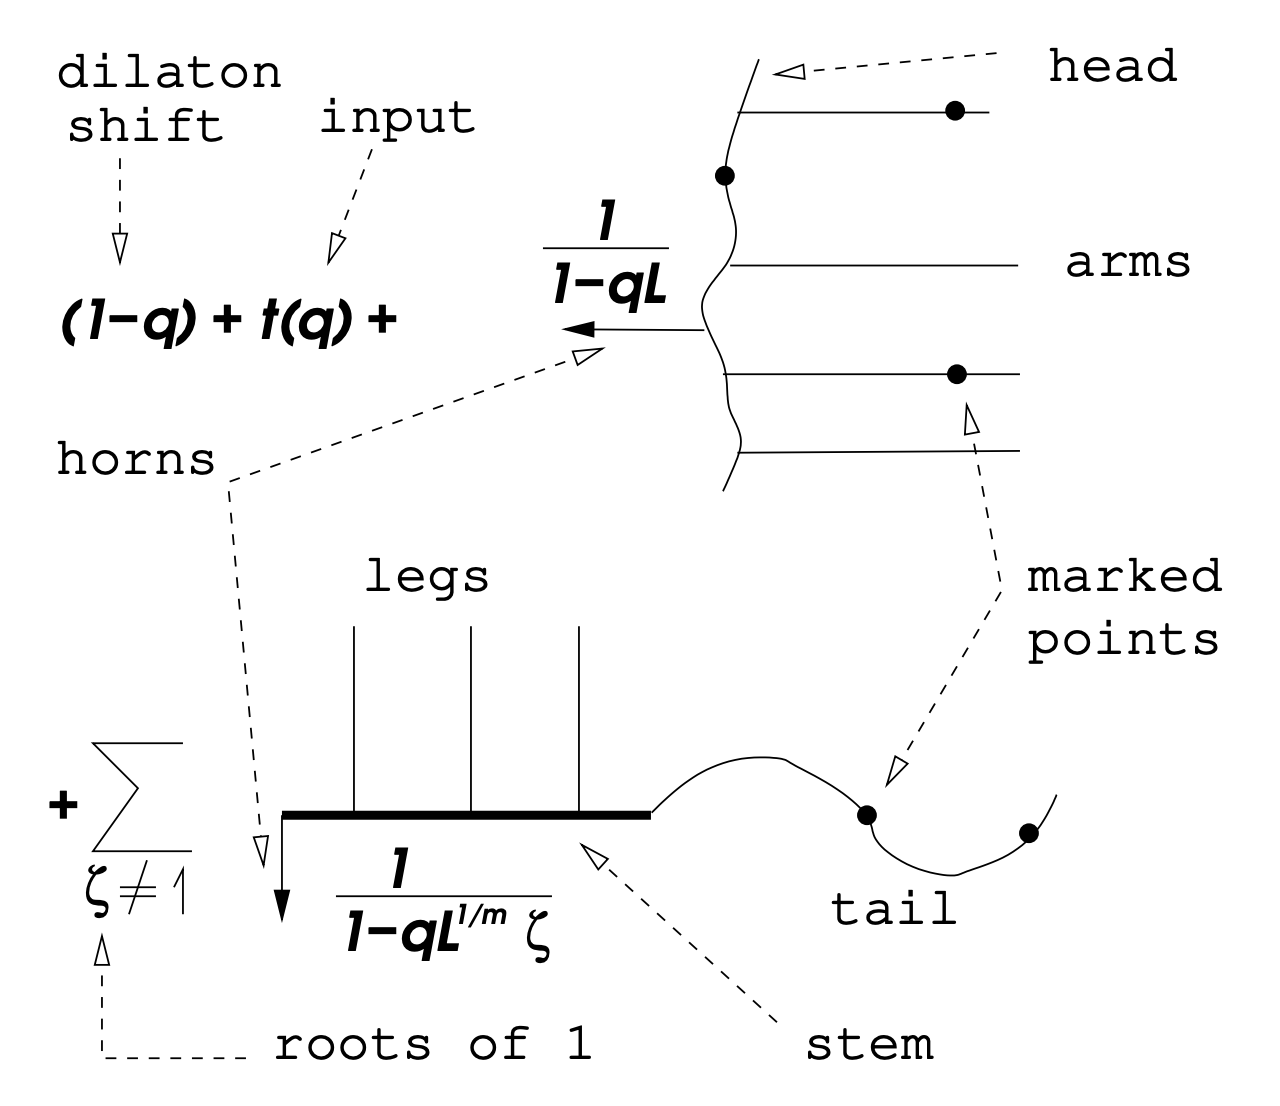
\includegraphics[width=0.8\textwidth]{givental.png}
    \caption{A way to keep track of the inertia components due to Givental-Tonita.}
    \label{fig:givental-png}
\end{figure}

\begin{figure}[htpb]
    \centering
    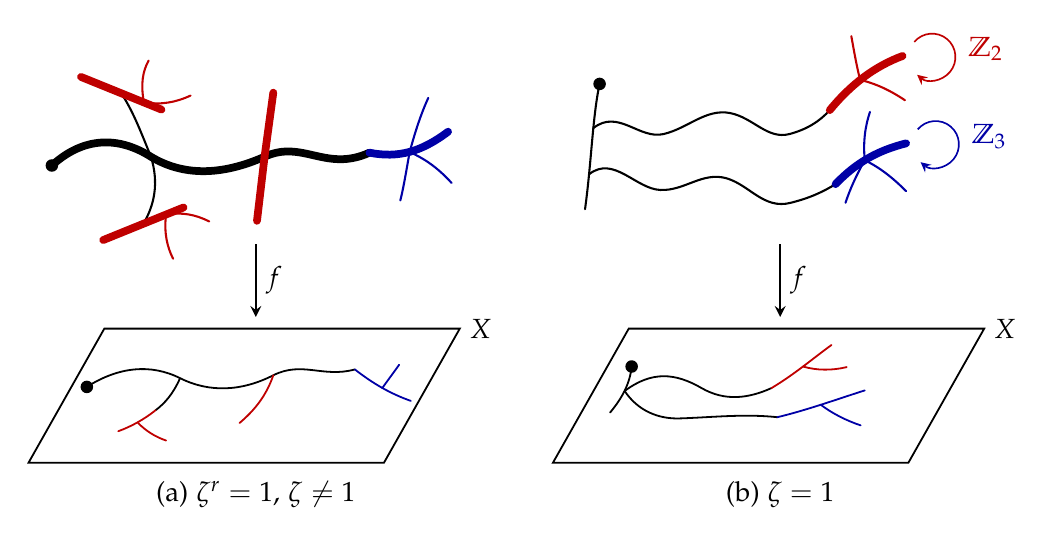
\begin{tikzpicture}[
        x=.74cm, y=.74cm,
        % Components of the domain curve. A cover style means the component
        % is a multiple cover of its image, drawn thick.
        dom/.style      ={black,         line width=.75pt, line cap=round},
        domcover/.style ={black,         line width=2.8pt, line cap=round},
        redcover/.style ={red!75!black,  line width=2.8pt, line cap=round},
        redtwig/.style  ={red!75!black,  line width=.75pt, line cap=round},
        bluecover/.style={blue!65!black, line width=2.8pt, line cap=round},
        bluetwig/.style ={blue!65!black, line width=.75pt, line cap=round},
        % Everything downstairs in X is drawn thin.
        img/.style      ={black,         line width=.65pt, line cap=round},
        redimg/.style   ={red!75!black,  line width=.65pt, line cap=round},
        blueimg/.style  ={blue!65!black, line width=.65pt, line cap=round},
        grparrow/.style ={->, >=stealth, line width=.6pt},
        fmap/.style     ={->, >=stealth, line width=.75pt},
        bull/.style     ={circle, fill=black, inner sep=1.6pt},
    ]

    %%%%%%%%%%%%%%%%%%%%%%%%%%%%%%%%%%%%%%%%%%%%%%%%%%%%%%%%%%%%%%%%%%%%%%%
    %% (a) zeta a primitive r-th root of unity, r >= 2.
    %%%%%%%%%%%%%%%%%%%%%%%%%%%%%%%%%%%%%%%%%%%%%%%%%%%%%%%%%%%%%%%%%%%%%%%
    \begin{scope}
        % The distinguished component: here g^r acts trivially on it, but g
        % does not, so it is a multiple cover of its image.
        \node[bull] at (-3.5,1.9) {};
        \draw[domcover]
            (-3.5,1.9)
            .. controls (-2.95,2.40) and (-2.35,2.40) .. (-1.80,2.05)
            .. controls (-1.25,1.72) and (-0.60,1.72) .. ( 0.15,2.05)
            .. controls ( 0.80,2.35) and ( 1.20,1.78) .. ( 1.95,2.12);

        % A leg meeting the distinguished component at a balanced node,
        % sticking out on both sides.  Each end carries a red multiple cover
        % together with the two branches interchanged by its automorphism.
        \draw[dom] (-1.80,2.05) .. controls (-2.00,2.55) and (-2.12,2.85) .. (-2.31,3.14);
        \draw[redcover] (-3.00,3.42) -- (-1.62,2.86);
        \draw[redtwig] (-1.92,2.98) .. controls (-1.98,3.30) and (-1.94,3.52) .. (-1.84,3.70);
        \draw[redtwig] (-1.92,2.98) .. controls (-1.62,2.94) and (-1.38,2.98) .. (-1.12,3.10);

        \draw[dom] (-1.80,2.05) .. controls (-1.66,1.60) and (-1.74,1.22) .. (-1.93,0.90);
        \draw[redcover] (-2.62,0.62) -- (-1.24,1.18);
        \draw[redtwig] (-1.54,1.06) .. controls (-1.58,0.74) and (-1.52,0.50) .. (-1.42,0.30);
        \draw[redtwig] (-1.54,1.06) .. controls (-1.26,1.10) and (-1.04,1.06) .. (-0.80,0.94);

        % A second balanced node, where the two legs are themselves the
        % multiple covers.
        \draw[redcover] (0.15,2.05) -- (0.30,3.15);
        \draw[redcover] (0.15,2.05) -- (0.02,0.95);

        % The tail: the part cut off at the unbalanced node.
        \draw[bluecover]
            (1.95,2.12) .. controls (2.45,2.02) and (2.85,2.14) .. (3.30,2.48);
        \draw[bluetwig] (2.64,2.13) .. controls (2.74,2.50) and (2.84,2.80) .. (2.96,3.06);
        \draw[bluetwig] (2.64,2.13) .. controls (2.58,1.80) and (2.54,1.54) .. (2.48,1.30);
        \draw[bluetwig] (2.64,2.13) .. controls (2.94,2.00) and (3.16,1.82) .. (3.36,1.60);

        \draw[fmap] (0,0.55) -- node[right] {$f$} (0,-0.70);

        % The target and the image of the map.
        \draw[img] (-3.9,-3.2) -- (2.2,-3.2) -- (3.5,-0.9) -- (-2.6,-0.9) -- cycle;
        \node[right] at (3.5,-0.9) {$X$};
        \node[bull] at (-2.90,-1.90) {};
        \draw[img] (-2.90,-1.90)
            .. controls (-2.35,-1.55) and (-1.80,-1.50) .. (-1.30,-1.75)
            .. controls (-0.80,-2.00) and (-0.25,-1.98) .. ( 0.30,-1.70)
            .. controls ( 0.80,-1.45) and ( 1.15,-1.75) .. ( 1.70,-1.60);
        % The two branches upstairs are folded onto the single one downstairs.
        \draw[img]    (-1.30,-1.75) .. controls (-1.42,-2.02) and (-1.56,-2.18) .. (-1.72,-2.30);
        \draw[redimg] (-1.72,-2.30) .. controls (-1.92,-2.46) and (-2.14,-2.58) .. (-2.36,-2.66);
        \draw[redimg] (-2.02,-2.52) .. controls (-1.88,-2.66) and (-1.72,-2.76) .. (-1.54,-2.82);
        \draw[redimg] ( 0.30,-1.70) .. controls ( 0.18,-2.05) and (-0.02,-2.30) .. (-0.28,-2.52);
        \draw[blueimg] (1.70,-1.60) .. controls (2.02,-1.85) and (2.32,-2.02) .. (2.66,-2.14);
        \draw[blueimg] (2.17,-1.92) .. controls (2.27,-1.78) and (2.36,-1.66) .. (2.46,-1.52);

        \node at (0,-3.75) {(a) \(\zeta^r = 1\), \(\zeta \neq 1\)};
    \end{scope}

    %%%%%%%%%%%%%%%%%%%%%%%%%%%%%%%%%%%%%%%%%%%%%%%%%%%%%%%%%%%%%%%%%%%%%%%
    %% (b) zeta = 1.
    %%%%%%%%%%%%%%%%%%%%%%%%%%%%%%%%%%%%%%%%%%%%%%%%%%%%%%%%%%%%%%%%%%%%%%%
    \begin{scope}[shift={(9,0)}]
        % Now g acts trivially on the distinguished component, so it is drawn
        % thin: it maps isomorphically onto its image.
        \node[bull] at (-3.10,3.30) {};
        \draw[dom] (-3.10,3.30) .. controls (-3.22,2.75) and (-3.24,1.95) .. (-3.35,1.15);
        \draw[dom] (-3.21,2.54)
            .. controls (-2.78,2.88) and (-2.42,2.34) .. (-2.00,2.44)
            .. controls (-1.58,2.54) and (-1.28,2.88) .. (-0.86,2.80)
            .. controls (-0.46,2.72) and (-0.22,2.34) .. ( 0.16,2.44)
            .. controls ( 0.46,2.52) and ( 0.68,2.66) .. ( 0.85,2.85);
        \draw[dom] (-3.28,1.75)
            .. controls (-2.86,2.08) and (-2.48,1.50) .. (-2.06,1.48)
            .. controls (-1.64,1.46) and (-1.34,1.80) .. (-0.92,1.68)
            .. controls (-0.52,1.56) and (-0.28,1.14) .. ( 0.18,1.26)
            .. controls ( 0.50,1.34) and ( 0.72,1.44) .. ( 0.95,1.58);

        % The arms: g acts nontrivially on them, through the indicated cyclic
        % group, which interchanges the thin branches sticking out.
        \draw[redcover] (0.85,2.85) .. controls (1.22,3.30) and (1.62,3.60) .. (2.10,3.78);
        \draw[redtwig] (1.37,3.37) .. controls (1.30,3.66) and (1.26,3.90) .. (1.22,4.12);
        \draw[redtwig] (1.37,3.37) .. controls (1.66,3.30) and (1.90,3.18) .. (2.14,3.02);
        \draw[grparrow, red!75!black]
            (2.30,4.02) arc[start angle=140, end angle=-130, radius=.40];
        \node[red!75!black, right] at (3.06,3.90) {$\Z_2$};

        \draw[bluecover] (0.95,1.58) .. controls (1.30,1.95) and (1.68,2.16) .. (2.16,2.28);
        \draw[bluetwig] (1.45,1.99) .. controls (1.42,2.32) and (1.46,2.58) .. (1.54,2.82);
        \draw[bluetwig] (1.45,1.99) .. controls (1.72,1.86) and (1.94,1.68) .. (2.16,1.46);
        \draw[bluetwig] (1.45,1.99) .. controls (1.30,1.72) and (1.20,1.50) .. (1.12,1.26);
        \draw[grparrow, blue!65!black]
            (2.36,2.52) arc[start angle=140, end angle=-130, radius=.40];
        \node[blue!65!black, right] at (3.12,2.40) {$\Z_3$};

        \draw[fmap] (0,0.55) -- node[right] {$f$} (0,-0.70);

        % The target and the image of the map.
        \draw[img] (-3.9,-3.2) -- (2.2,-3.2) -- (3.5,-0.9) -- (-2.6,-0.9) -- cycle;
        \node[right] at (3.5,-0.9) {$X$};
        \node[bull] at (-2.55,-1.55) {};
        \draw[img] (-2.55,-1.55) .. controls (-2.58,-1.85) and (-2.72,-2.10) .. (-2.92,-2.34);
        \draw[img] (-2.67,-1.97)
            .. controls (-2.20,-1.62) and (-1.80,-1.66) .. (-1.35,-1.92)
            .. controls (-0.95,-2.15) and (-0.55,-2.10) .. (-0.15,-1.92);
        \draw[img] (-2.67,-1.97)
            .. controls (-2.45,-2.30) and (-2.10,-2.46) .. (-1.70,-2.44)
            .. controls (-1.15,-2.42) and (-0.60,-2.36) .. (-0.05,-2.42);
        % Each arm is folded onto a single image curve with one branch.
        \draw[redimg] (-0.15,-1.92) .. controls (0.25,-1.68) and (0.55,-1.42) .. (0.88,-1.18);
        \draw[redimg] ( 0.39,-1.55) .. controls (0.63,-1.62) and (0.89,-1.62) .. (1.14,-1.56);
        \draw[blueimg] (-0.05,-2.42) .. controls (0.45,-2.30) and (0.95,-2.12) .. (1.45,-1.96);
        \draw[blueimg] ( 0.70,-2.21) .. controls (0.90,-2.36) and (1.14,-2.48) .. (1.38,-2.56);

        \node at (0,-3.75) {(b) \(\zeta = 1\)};
    \end{scope}
    \end{tikzpicture}
    \caption{The components of \(I\bar{M}_{0,1}(X,\beta)\), due to You-Cheng.}
    \label{fig:adelic-components}
\end{figure}

We will now explain~\Cref{fig:adelic-components}. Let \(L_1\) be the cotangent line at the first marked point and let \(g\) be the automorphism of a point of \(I\bar{M}_{0,1}(X,\beta)\). Then \(\zeta\) is defined by the condition that \(g\) acts on \(L_1\) with eigenvalue \(\zeta\). In both pictures, the bullet denotes the first marked point and its image in \(X\), while a thick component is one which is a multiple cover of its image.

First, suppose that \(\zeta = 1\). Then the black component is the maximal connected component containing the first marked point on which \(g\) acts as the identity. The red and blue components are precisely those on which \(g\) acts nontrivially, and we refer to them as \textit{arms}.

Now suppose that \(\zeta\) is an \(r\)-th root of unity for some \(r \geq 2\). In this case, the nodes of the black component are required to be balanced with respect to the \(g\)-action, so we cut off the nonbalanced part, which is colored blue, and refer to it as the \textit{tail}. On what remains, the black component is the maximal connected component containing the first marked point on which \(g^r\) acts as the identity. Finally, after taking out the black component and the tail, we refer to the remaining components as \textit{legs}.

% \begin{figure}[htpb]
%     \centering
%     \resizebox{\textwidth}{!}{%
%     \begin{tikzpicture}[
%         x=1cm,
%         y=1cm,
%         curve/.style={black, line width=1.25pt, line cap=round},
%         fixed component/.style={black, line width=3.2pt, line cap=round},
%         red component/.style={red!75!black, line width=3.2pt, line cap=round},
%         blue component/.style={blue!70!black, line width=3.2pt, line cap=round},
%         image curve/.style={black, line width=1.05pt, line cap=round},
%         action arrow/.style={->, >=stealth, line width=.75pt},
%         map arrow/.style={->, >=stealth, line width=.8pt},
%         marked point/.style={circle, fill=black, inner sep=1.8pt}
%     ]
%         % The case of a nontrivial r-th root of unity.
%         \begin{scope}[xshift=0cm]
%             \node[font=\large] at (0,5.95)
%                 {$r\geq 2,\qquad \zeta^r=1,\quad \zeta\neq 1$};
%
%             % Domain curve.
%             \node[marked point] (p1) at (-3.15,3.7) {};
%             \draw[fixed component]
%                 (p1) .. controls (-2.25,4.15) and (-1.55,4.2) ..
%                 (-1.15,3.92)
%                 .. controls (-0.55,3.45) and (0.35,3.45) ..
%                 (0.85,3.82)
%                 .. controls (1.35,3.35) and (1.85,3.45) ..
%                 (2.2,4.05);
%             \fill (-1.15,3.92) circle (2.2pt);
%             \fill (0.85,3.82) circle (2.2pt);
%             \fill (2.2,4.05) circle (2.2pt);
%
%             % Two legs attached to balanced nodes.
%             \draw[curve]
%                 (-1.15,3.92) .. controls (-1.25,4.45) and (-1.35,4.78) ..
%                 (-1.72,5.18);
%             \draw[red component]
%                 (-2.18,5.48) .. controls (-1.92,5.25) and (-1.65,5.08) ..
%                 (-1.36,5.02);
%             \draw[curve, red!75!black]
%                 (-1.67,5.14) .. controls (-1.64,5.35) and (-1.59,5.55) ..
%                 (-1.53,5.72);
%             \draw[curve, red!75!black]
%                 (-1.53,5.08) .. controls (-1.34,5.14) and (-1.18,5.25) ..
%                 (-1.02,5.4);
%             \draw[action arrow, red!75!black]
%                 (-1.9,5.38) arc[start angle=20,end angle=315,radius=.42];
%
%             \draw[curve]
%                 (-1.15,3.92) .. controls (-1.1,3.35) and (-1.25,3.0) ..
%                 (-1.62,2.63);
%             \draw[red component]
%                 (-2.18,2.32) .. controls (-1.9,2.56) and (-1.6,2.75) ..
%                 (-1.3,2.84);
%             \draw[curve, red!75!black]
%                 (-1.65,2.68) .. controls (-1.62,2.48) and (-1.59,2.25) ..
%                 (-1.54,2.06);
%             \draw[curve, red!75!black]
%                 (-1.5,2.76) .. controls (-1.31,2.7) and (-1.14,2.58) ..
%                 (-.98,2.42);
%             \draw[action arrow, red!75!black]
%                 (-1.85,2.57) arc[start angle=25,end angle=315,radius=.38];
%
%             % A second symmetric pair of balanced legs.
%             \draw[curve] (0.2,3.48) .. controls (0.16,4.05) and (0.2,4.35) ..
%                 (0.32,4.7);
%             \draw[red component] (0.2,3.9) -- (0.33,4.72);
%             \draw[curve] (0.2,3.48) .. controls (0.16,3.12) and (0.08,2.82) ..
%                 (-0.02,2.48);
%             \draw[red component] (0.11,3.05) -- (-0.03,2.46);
%
%             % The nonbalanced tail.
%             \draw[blue component]
%                 (2.2,4.05) .. controls (2.68,3.92) and (3.05,4.02) ..
%                 (3.48,4.3);
%             \draw[curve, blue!70!black] (2.86,4.08) -- (3.15,4.78);
%             \draw[curve, blue!70!black] (2.95,4.07) -- (2.88,3.35);
%             \draw[curve, blue!70!black] (2.95,4.07) -- (3.45,3.55);
%
%             % The target and the image of the map.
%             \draw[curve]
%                 (-3.55,-1.65) -- (2.48,-1.65) -- (3.48,1.0) --
%                 (-2.65,1.0) -- cycle;
%             \node[marked point] (xp1) at (-2.65,-0.25) {};
%             \draw[image curve]
%                 (xp1) .. controls (-2.05,0.04) and (-1.55,.22) ..
%                 (-1.15,.12)
%                 .. controls (-.5,-.05) and (-.2,-.1) ..
%                 (.12,.18)
%                 .. controls (.55,.55) and (1.0,.62) ..
%                 (1.55,.45);
%             % The first red orbit maps to a black connector followed by
%             % one red image curve; its two thin branches fold to the
%             % smaller red branch.
%             \draw[image curve]
%                 (-1.15,.12) .. controls (-1.23,-.08) and (-1.34,-.23) ..
%                 (-1.48,-.32);
%             \draw[red!75!black, line width=1.05pt, line cap=round]
%                 (-1.48,-.32) .. controls (-1.62,-.45) and (-1.78,-.58) ..
%                 (-1.92,-.65);
%             \draw[red!75!black, line width=1.05pt, line cap=round]
%                 (-1.69,-.51) .. controls (-1.58,-.64) and (-1.45,-.72) ..
%                 (-1.31,-.76);
%             \draw[red!75!black, line width=1.05pt, line cap=round]
%                 (.12,.18) .. controls (.02,-.22) and (-.25,-.38) ..
%                 (-.48,-.63);
%             \draw[blue!70!black, line width=1.05pt, line cap=round]
%                 (1.05,.57) .. controls (1.35,.12) and (1.68,-.18) ..
%                 (2.08,-.38);
%             \draw[blue!70!black, line width=1.05pt, line cap=round]
%                 (1.78,-.2) .. controls (1.82,-.08) and (1.88,.04) ..
%                 (1.96,.15);
%             \draw[map arrow] (0,2.62) -- node[right] {$f$} (0,1.22);
%             \node at (0,-2.1) {$(a)\ \zeta\neq 1$};
%         \end{scope}
%
%         % The untwisted eigenvalue case.
%         \begin{scope}[xshift=8.25cm]
%             \node[font=\large] at (0,5.95)
%                 {$I\overline{\mathcal M}_{0,1}(X,\beta),\qquad
%                   \on{Tr} g|_{L_1}=\zeta$};
%
%             % Domain curve: the thick portions have multiple covers onto
%             % their images.
%             \node[marked point] (p2) at (-2.95,4.45) {};
%             \draw[fixed component]
%                 (p2) .. controls (-3.08,3.85) and (-3.08,3.18) ..
%                 (-3.18,2.65);
%             \draw[curve]
%                 (-3.02,3.9) .. controls (-2.42,4.05) and (-2.0,3.62) ..
%                 (-1.62,3.72)
%                 .. controls (-1.18,3.3) and (-.72,3.18) ..
%                 (-.2,3.32);
%             \draw[curve]
%                 (-3.13,3.25) .. controls (-2.6,3.52) and (-2.25,2.88) ..
%                 (-1.8,2.68)
%                 .. controls (-1.25,2.4) and (-.68,2.42) ..
%                 (-.15,2.48);
%
%             % Nontrivial arms, shown in red and blue.
%             \draw[curve]
%                 (-.2,3.32) .. controls (.3,3.48) and (.5,3.72) ..
%                 (.76,3.92);
%             \draw[red component]
%                 (.76,3.92) .. controls (1.1,4.42) and (1.5,4.72) ..
%                 (2.02,4.9);
%             \draw[curve, red!75!black]
%                 (1.12,4.4) .. controls (1.08,4.68) and (1.05,4.92) ..
%                 (1.02,5.18);
%             \draw[curve, red!75!black]
%                 (1.55,4.7) .. controls (1.82,4.62) and (2.04,4.48) ..
%                 (2.25,4.3);
%             \draw[action arrow, red!75!black]
%                 (1.6,4.88) arc[start angle=210,end angle=-35,radius=.48];
%             \node[red!75!black, left] at (1.02,5.08) {$\Z_2$};
%
%             \draw[curve]
%                 (-.15,2.48) .. controls (.28,2.45) and (.55,2.64) ..
%                 (.86,2.76);
%             \draw[blue component]
%                 (.86,2.76) .. controls (1.18,3.13) and (1.52,3.32) ..
%                 (2.0,3.42);
%             \draw[curve, blue!70!black]
%                 (1.27,3.13) .. controls (1.34,3.4) and (1.43,3.65) ..
%                 (1.55,3.9);
%             \draw[curve, blue!70!black]
%                 (1.57,3.33) .. controls (1.83,3.2) and (2.05,3.02) ..
%                 (2.27,2.82);
%             \draw[action arrow, blue!70!black]
%                 (1.9,3.37) arc[start angle=145,end angle=-120,radius=.43];
%             \node[blue!70!black, above] at (2.55,3.62) {$\Z_3$};
%
%             % Target X and the images of the colored components.
%             \draw[curve]
%                 (-3.55,-1.65) -- (2.48,-1.65) -- (3.48,1.0) --
%                 (-2.65,1.0) -- cycle;
%             \node[marked point] (xp2) at (-2.05,.02) {};
%             \draw[image curve]
%                 (xp2) .. controls (-2.0,-.32) and (-2.35,-.62) ..
%                 (-2.62,-.93);
%             \draw[image curve]
%                 (-2.25,-.52) .. controls (-1.82,-.12) and (-1.55,-.12) ..
%                 (-1.14,-.42)
%                 .. controls (-.88,-.62) and (-.54,-.63) ..
%                 (-.22,-.52);
%             \draw[image curve]
%                 (-2.25,-.52) .. controls (-2.58,-.44) and (-2.75,-.62) ..
%                 (-2.98,-.83);
%             \draw[red!75!black, line width=1.05pt]
%                 (-.22,-.52) .. controls (.22,-.13) and (.5,.22) ..
%                 (.82,.48);
%             % The two thin red branches upstairs fold to this one
%             % additional branch of the red image curve.
%             \draw[red!75!black, line width=1.05pt, line cap=round]
%                 (.345,.029) .. controls (.57,-.02) and (.77,.06) ..
%                 (1.0,.18);
%             % A chain of black components joins the blue image to the
%             % distinguished black component.
%             \draw[image curve]
%                 (-2.25,-.52) .. controls (-2.12,-.76) and (-2.0,-.91) ..
%                 (-1.88,-1.0);
%             \draw[image curve]
%                 (-1.88,-1.0) .. controls (-1.76,-.82) and (-1.53,-.91) ..
%                 (-1.38,-1.18);
%             \draw[image curve]
%                 (-1.38,-1.18) .. controls (-.65,-.76) and (.08,-.68) ..
%                 (.78,-.72);
%             \draw[blue!70!black, line width=1.05pt, line cap=round]
%                 (.78,-.72) .. controls (1.24,-.74) and (1.58,-.62) ..
%                 (1.98,-.32);
%             \draw[map arrow] (0,2.03) -- node[right] {$f$} (0,1.22);
%             \node at (0,-2.1) {$(b)\ \zeta=1$};
%         \end{scope}
%     \end{tikzpicture}%
%     }
%     \caption{The decomposition of a component of
%     \(I\overline{\mathcal M}_{0,1}(X,\beta)\) into its distinguished
%     component, legs or arms, and tail, provided by You-Cheng. Thick curves indicate components
%     that map with degree greater than one onto their images. Symmetric
%     branches occur on the domain, and \(f\) folds each orbit to a single
%     image curve in \(X\).}
%     \label{fig:adelic-components}
% \end{figure}
%
% We will now explain the meaning of the different parts of~\Cref{fig:adelic-components}. Let \(L_1\)
% be the cotangent line at the first marked point and define \(\zeta\) by
% \[
%     g|_{L_1}=\zeta\,\mr{Id}_{L_1}.
% \]
% The bullets denote the first marked point and its image in \(X\), and a
% thick curve denotes a component that is a multiple cover of its image.
% The black component is the maximal connected component containing the
% first marked point on which \(g\) acts trivially when \(\zeta=1\). The red
% and blue components on which \(g\) acts nontrivially are called
% \textit{arms}.
%
% More generally, suppose that \(\zeta\) is an \(r\)-th root of unity with
% \(r\geq 2\). The nodes of the thick black component must be balanced with
% respect to the \(g\)-action. Cut off the part attached at an unbalanced
% node (the blue component in the figure); this part is called the
% \textit{tail}. In what remains, the thick black component is the maximal
% connected component containing the first marked point on which \(g^r\)
% acts trivially. After removing the black component and the tail, the
% remaining components are called \textit{legs}.

The following definition is due to Givental. We write
\[ \ab<\frac{\Phi}{1-qL}>_{0,1,\beta}^{X,K} \coloneqq \sum_{\zeta} \ab<\frac{\Phi}{1-qL}>_{0,1,\beta}^{X_{\zeta}}, \]
where the \(X_{\zeta}\) term is simply the contribution of \(M_{\zeta}\) under the Riemann-Roch theorem. Now, we will define arms, legs, and tails. Here, we define the \textit{arms}
\[ \mr{arm}(q) \coloneqq \sum_{\beta, \alpha, \zeta \neq 1} Q^{\beta} \Phi^{\alpha}\ab<\frac{\Phi}{1-qL}>_{0,1,\beta}^{X_{\zeta}}, \]
the \textit{legs}
\[ \mr{leg}_{\zeta}(q) \coloneqq \mr{leg}_r(q) = \Psi^r (\mr{arm}(q)), \]
and the \textit{tails}
\[ \mr{tail}_{\zeta}(q) \coloneqq \sum_{\beta, \alpha, \zeta' \neq \zeta} Q^{\beta} \Phi^{\alpha} \ab<\frac{\Phi^{\alpha}}{1-qL}>_{0,1,\beta}^{X_{\zeta'}}. \]

\begin{prop}
    The Laurent expansion of the J-function at \(q = 1\) is given by
    \begin{align*}
        J^K(0)_{q=1} &= J^{\mr{fake}}(\mr{arm}(q)) \\
        &\coloneqq 1-q + \mr{arm}(q) + \sum_{n,\beta,\alpha} \ab<\frac{1}{1-qL}, \mr{arm}(L), \ldots, \mr{arm}(L)>_{0,n+1,\beta}^{\mr{fake}},
    \end{align*}
    where the fake invariants are computed by applying Riemann-Roch and only considering the contribution of the untwisted sector.
\end{prop}

\begin{prop}
    At any other root of unity \(\zeta \neq 1\), we have
    \begin{align*}
        &J^K(0)_{q = \zeta} = (1-q) + \mr{tail}_{\zeta}(q) \\
        &+ \sum_{n,\beta,\alpha} \frac{Q^{r\beta}\Phi^{\alpha}}{n!} \ab[\frac{\Phi_{\alpha}}{1-\zeta q L^{1/r}}, \mr{leg}_r(L), \ldots, \mr{leg}_r(L), 1 - \zeta^{-1}L^{1/r} + \mr{tail}_{\zeta}(\zeta^{-1} L^{1/r})]^{\mr{stem}},
    \end{align*}
    where the stem is some fake invariant of \(X \times B\mu_r\) defined on the moduli space
    \[ \bar{M}_{-,n+2,\beta}^X(\beta) \coloneqq \bar{M}_{0,2}(X \times B\mu_r, \beta, (g, 1, \ldots, 1, g^{-1})). \]
    It is defined by the formula
    \begin{align*}
        [\cdots]^{\mr{stem}} \coloneqq \int_{[\bar{M}_{0,n+2,\beta}^X(\zeta)]^{\vir}} \on{td}(T_{\bar{M}}) \on{ch}\ab(\frac{\on{Tr}(\cdots)}{\on{Tr}(\lambda_{-1}(N^*))}), 
    \end{align*}
    where \(N\) denotes the normal bundle of \(\bar{M}_{0,n+2,\beta}^X(\zeta) \subset \bar{M}_{0,nr+2}(X, r\beta)\).
\end{prop}

\begin{rmk}
    If we can calculate the fake and stem theories, then we can compute genus zero quantum K invariants.
\end{rmk}

\subsection{Quantum K-theory of a point}%
\label{sub:Quantum K-theory of a point}

One natural question is to study higher genus quantum K-theory. We will begin with the simplest target, which is a point. One motivation for studying higher-genus would be to try to prove integrality of the Klemm-Pandharipande definition of GV invariants for Calabi-Yau fourfolds or the Pandharipande-Zinger definition of GV invariants for Calabi-Yau fivefolds (in this situation, we only need to consider genus \(1\)). One reason we need to consider the quantum K-theory of a point is because in \(I\bar{M}_{1,1}(X, \beta)\), there are some components where an entire curve of genus \(1\) is contracted to a point.

\begin{quest}
    What is the K-theoretic Witten-Kontsevich theorem?\footnote{According to You-Cheng, the difficulty lies everywhere.}
\end{quest}

We will first recall the cohomological Witten's conjecture. We will begin with the operator
\[ L = \partial_x^2 + u(x) \]
and deform it to
\[ \tilde{L} = \partial_x^2 + u(x, T_3, T_5, \ldots), \]
where we should think of \(x = T_1\) and \(u(x) = u(x, 0, 0,\ldots)\). Formally, write
\[ L^{1/2} = \partial_x + \sum_{k > 0} a_{-k}(x) \partial_x^{-k} \]
using the property
\[ \partial^n \circ f = \sum_{m = 0}^{\infty} \binom{n}{m} f^{(m)} \partial^{n-m} \]
for all integers \(n \in \Z\). In particular, we construct the (2-)KdV hierarchy by the equation
\[ \pdv{\tilde{L}}{T_{2k+1}} = \ab[(\tilde{L}^{\frac{2k+1}{2}})_{\geq 0}, \tilde{L}] \]
for all \(k \geq 0\). We define a \textit{\(\tau\)-function} to be a function \(\tau\) such that 
\[ 2 \pdv[2]{}{x}\log \tau(x, T_3, T_5, \ldots) = u(x, T_3, T_5, \ldots). \]
Now perform the above process using \(u = 2x\). Define the function
\[ F(t_0, t_1, \ldots) \coloneqq \sum_{n \geq 0} \sum_{k_0, \ldots, k_n} \ab<\tau_0^{k_0} \cdots \tau_n^{k_n}> \frac{t_0^{k_0} \cdots t_n^{k_n}}{k_0! \cdots k_n!}. \]
Note that because the genus is determined entirely by the number of insertions and the degree of the insertions, the notation
\[ \ab<\tau_0^{k_0} \cdots \tau_n^{k_n}> \]
uniquely determines a descendant GW invariant of a point.

\begin{thm}[Kontsevich]
    F is a \(\tau\)-function of the KdV hierarchy constructed starting with \(L = \partial_x^2 + 2x\) under the change of variables \(t_i = (2i+1)!! T_{2i+1}\).
\end{thm}

One application of this theorem is to consider virtual localization. For example, suppose we consider \(\bar{M}_{g,0}(X, d[C])\) where \(C\) is a unique rational curve in a Calabi-Yau threefold with normal bundle \(N = \mc{O}(-1)\oplus \mc{O}(-1)\). Then in this setting we can reduce to the local model and compute
\begin{align*}
    \int_{[\bar{M}_{g,0}(\P^1, d)]^{\vir}} c_{\mr{top}}(R^1 \pi_* N) = \sum_{m \vdash d} \frac{(-1)^{d-L(m)}}{\abs{\Aut(m)}} \prod_{i=1}^{L(m)} \int_{\bar{M}_{g, L(m)}} \frac{1 + \cdots + c_g(\mc{H})}{\prod_i (1-m_i \psi_i)}
\end{align*}
via virtual localization. If we would like a similar result in K-theory, then we will need to consider terms of the form
\[ \chi\ab(\bar{M}_{g, L(m)}/\Aut(m), \frac{\lambda_{-1}(\mc{H})}{1-m_i L_i}), \]
so we will need to consider the permutation-equivariant quantum K-theory of a point.

We now proceed with a literature review. First, Lee computed the formula
\[ \ab<\frac{1}{1-q_1 L}, \ldots, \frac{1}{1-q_n L}>_{0,n}^{\mr{pt}, K} = \ab(\prod_{i=1}^n \frac{1}{1-q_i}) \ab(1 + \sum_{i=1}^n \frac{q_i}{1-q_i})^{n-3}. \]
Later, Lee-Qu gave a way to compute
\[ \ab<\frac{1}{1-q_1 L}, \ldots, \frac{1}{1-q_n L}>_{1,n}^{\mr{pt}, K} \]
in principle. Givental computed the formula
\[ \sum_{n \geq 2} \ab<\frac{1}{1-q L}, 1, \ldots, 1>_{0,1+n}^{S_n} = (1-q) \exp\ab(\sum_{k > 0} \frac{\Psi^k}{k} \ab(1 + \frac{q}{1-q})). \]
Finally, in 2024, Milanov computed 
\begin{align*}
    \sum_{n \geq 0}& \ab<\frac{1}{1-q_1 L}, \ldots, \frac{1}{1-q_r L}, 1, \ldots, 1>_{0,r+n}^{S_n} \\
    &= \ab(\prod_{i=1}^{r} \frac{1}{1-q_i})\ab(1 + \sum_{i=1}^r \frac{q_i}{1-q_i}) \exp\ab(\frac{\Psi^k}{k} \ab(1 + \sum_{i=1}^r \frac{q_i}{1-q_i})). 
\end{align*}

Let \(s \in \Z\) and define the pluri-Hodge sheaf \(\mc{H}_s \coloneqq R^0 \pi_* (\omega_{\pi}^s)\). Considering the map \(\bar{M}_{g,n+1} \xrightarrow{\pi} \bar{M}_{g,n}\), we will denote the upstairs cotangent lines by \(L_i\) and the downstairs ones by \(\ell_i\).

\begin{lem}
    For all integers \(s\) and \(d_i\), we have
    \[ \pi_*\ab(\omega_{\pi}^s\ab(\sum_{i=1}^r d_i D_i)) = \mc{H}_s \mc{H}_{1-s}^* + \sum_{i=1}^n \sum_{k=1}^{d_i} \ell_i^{-k+s}. \]
\end{lem}

\begin{rmk}
    Note that if \(f(q) \in \Z[q]\), then \(\exp \sum_k \frac{\Psi^k}{k} (f(q)) \in \Z \ps{q}\). The reason is that this operation sends \(f = \sum_{i=1}^{n} a_i q^i\) to \(\prod_{i=1}^n \frac{1}{(1-q_i)^{a_i}}\).
\end{rmk}

\begin{proof}
    When all \(d_i\) are zero, we see that
    \[ R^0 \pi_* \omega_{\pi}^s - R^1 \pi_* \omega_{\pi}^s = \mc{H}_s - \mc{H}_{1-s}^* \]
    by Serre duality. The next step is to show that
    \[ \pi_* \omega_{\pi}^s ((r+1)D_i) = \pi_* \omega_{\pi}^s(r D_i) + \ell_i^{s-r-1}. \]
    Here, we first consider the exact sequence
    \[ 0 \to \mc{O} (-D_i) \to \mc{O} \to \mc{O}_{D_i} \to 0 \]
    and twist by \(\omega_{\pi}^s\) to obtain
    \[ 0 \to \omega_{\pi}^s(r D_i) \to \omega_{\pi}^s ((r+1)D_i) \to \omega_{\pi}^s ((r+1)D_i) \otimes \mc{O}_{D_i} \to 0 \]
    and then compute the pushforward.
\end{proof}

\begin{lem}
    Let \(f_i\) be rational functions, for example \(\frac{1}{1-q L}\). Then
    \begin{align*}
        \ab<f_1(L), \ldots, f_n(L), L_{n+1}^r>_{g, n+1} ={}& \sum_{i=1}^n \ab<f_1(L), \ldots, D(f_i f_{n+1}), \ldots, f_n(L_n)>_{g, n} \\
        &+ \ab<f_1(L), \ldots, f_n(L) \mid \mc{H}_r - \mc{H}_{1-r}^*>_{g,n},
    \end{align*}
    where \(f_{n+1} = L_{n+1^r}\) and \((Df)(x) \coloneqq \frac{f(x)-f(1)}{x-1}\).
\end{lem}

To prove this, we need to consider the pushforward
\begin{align*}
    \pi_* (L_1^{d_1} \cdots L_{n+1}^{d_{n+1}}) &= \pi_* \ab(\pi^*(\ell_1^{d_1} \otimes \cdots \otimes \ell_n^{d_n}) \otimes \omega_{\pi}^{d_{n+1}}(d_i+d_{n+1})D_i).
\end{align*}
Here, we use the fact that \(L_i = (\pi^* \ell_i)(D_i)\) and \(L_{n+1} = \omega_{\pi}(D_1 + \cdots + D_n)\). Applying the previous lemma, we see that the pushforward becomes
\[ (\ell_1^{d_1} \cdots \ell_n^{d_n})\ab(\mc{H}_{d_{n+1}} - \mc{H}_{1-d_{n+1}}^* + \sum_{i=1}^n \sum_{k=1}^{d_i + d_{n+1}} \ell_i^{-k+d_{n+1}}). \]
Now, Lee's formula computes the correlators
\[ \ab<(L-1)^{k_1}, \ldots, (L-1)^{k_n}>_{0,n} = \frac{(n-3)!}{\prod_{i=1}^n k_i \ab(n-3-\sum_i k_i)!} \]
via the expansion
\[ \frac{1}{1-qL} = \frac{1}{1-q} \sum_{k \geq 0} \frac{q^k(L-1)^k}{(1-q)^k}. \]
Note here that there is no Hodge bundle in genus \(0\), so in fact the lemma can be used to obtain Lee's formula.

\begin{lem}
    We have
    \[ \mc{H}_r - \mc{H}_{1-r}^* = \pi^* (\mc{H}_r - \mc{H}_{1-r}^*) - \sum_{i=1}^n (D^2 (\pi^* \ell_i)^r) \mc{O}_{D_i}. \]
\end{lem}

The lemmas collectively imply that we can reduce to the case of a single marking at the cost of making the insertions very complicated and introducing pluri-Hodge terms everywhere. In genus \(1\), life becomes easier because on \(\bar{M}_{1,1}\), we have 
\[ \mc{H}_r = \mc{O}(r) = L_1^r. \]
In this case, recall the classical formula
\[ \chi\ab(\bar{M}_{1,1}, \frac{1}{1-qL}) = \frac{1}{(1-q^4)(1-q^6)}. \]
Unfortunately, computing
\[ \chi\ab(\bar{M}_{1,n}; \frac{1}{1-q_1 L} \cdots \frac{1}{1-q_n L}) \]
is too hard, so we can try to compute
\[ \chi\ab(\bar{M}_{1,1}; \frac{1}{1-q_1 L_1} \cdots \frac{1}{1-q_n L_1})  \]
which is known, but it is unclear how to write a good formula for it. The reason we would consider this is the operation
\[ \Z\ps{q} \xrightarrow{[]_r} \Z\ps{q_1, \ldots, q_r} \qquad q^k \to h_k(q_1, \ldots, q_r) \coloneqq \sum_{\ell_1 + \cdots + \ell_r = k} q_1^{\ell_1} \cdots q_r^{\ell_r}. \]
Unfortunately, You-Cheng does not know how to write
\[ \chi\ab(\bar{M}_{1,1}; \frac{1}{1-q_1 L_1} \cdots \frac{1}{1-q_n L_1}) = \ab[\frac{1}{(1-q^4)(1-q^6)}]_n \]
in a nice form. In principle we can write formulae like
\[ [f(q)]_2 \coloneqq \frac{q_1 f(q_1) - q_2 f(q_2)}{q_1 - q_2}, \]
but this does not seem to help much.

\subsection{Permutation-equivariant theory of a point}%
\label{sub:Permutation-equivariant theory of a point}

We can compute \(\chi\ab(\bar{M}_{1,1}, \frac{1}{1-q L})\) in another way. Consider the involution on an elliptic curve, which gives a map
\[ \bar{M}_{1,1} \to \bar{M}_{0,1+3}/S_3. \]
Then, Givental computes
\[ \chi\ab([\bar{M}_{0,1+n-1}/S_{n-1}], \frac{1}{1-qL}) = \prod_{i=2}^{n-1} \frac{1}{1-q^i}. \]
In particular, we obtain
\[ \frac{1}{1-q^2} \cdots \frac{1}{1-q^3}, \]
and then because the map is a \(\mu_2\)-gerbe (or a \(2:1\)-cover on objects), we obtain the desired formula.

Consider \(\mc{H}_{g,1} \subset \bar{M}_{g,1}\) to be the hyperelliptic locus. Note that the marking lies on a Weierstrass point. Note that the fixed points of the hyperelliptic involution go to \(2g+1\) points on \(\P^1\), and therefore one would want to use the calculation
\[ \chi\ab(\bar{M}_{0,1+2g+1}/S_{2g+1}, \frac{1}{1-q L}) = \prod_{i=2}^{2g+1} \frac{1}{1-q^i} \]
to compute the quantity
\(\chi\ab(\mc{H}_{g,1}, \frac{1}{1-qL})\). However, because of the way that the curves upstairs degenerate, we will need to consider the Hassett moduli space where the last \(2g+1\) markings have weight \(\frac{1}{2}\).
 






\section{Quasimap wall-crossing (Yang Zhou)}%
\label{sec:Quasimap wall-crossing (Yang Zhou)}

Let \(X\) be the quintic threefold. Our goal is to count genus zero curves on \(X\), which is a problem that was solved by Givental and Lian-Liu-Yau. Via the closed immersion \(X \subset \P^4\), we can write
\[ \bar{M}_0(X, d) \subset \bar{M}_0(\P^4, d), \]
which is smooth and has a torus action by \((\C^{\times})^5\). If a map is fixed by this action, the domain must have some components which map to the fixed points and some components which form an \(n :1\) cover of the \(1\)-dimensional orbits. In particular, the fixed locus is indexed by a set of graphs.

In this setting, we have the quantum Lefschetz principle, which states that
\[ [\bar{M}_0(X, d)]^{\on{vir}} = e(E) \cap [\bar{M}_0(\P^4, d)]. \]
Here, the vector bundle \(E\) is defined by
\[ E = \pi_* f^* \mc{O}(5), \]
where \(\pi\) is the universal curve and \(f\) is the universal stable map. We will give a different perspective on the result that if
\begin{align*}
    I(q, z) &= 1 + \sum_{d > 0} \frac{\prod_{k=1}^5 (5H+kz)}{\prod_{k=1}^d (H+kz)^5} q^d \in H^*(X)[z^{-1}] \ps{q} \\
    &= I_0(q) \cdot 1 + I_1(q) \frac{H}{z} + \frac{I_2}(q) \frac{H^2}{z^2} + I_3(q) \frac{H^3}{z^3},
\end{align*}
then
\[ J (Q, z) = 1+ \sum_{d>0} \phi^{\alpha} \ab<\frac{\phi_{\alpha}}{z(z-\psi)}>_{0,1}^X Q^d = \frac{I}{I_0} \]
up to the mirror map \(Q = q \exp\ab(\frac{I_1}{I_0})\). 

\subsection{Naive counting}%
\label{sub:Naive counting}

We will consider ``maps'' \(\P^1 \to X \subset \P^4\) from a fixed \(\P^1\). For simplicity, we will assume \(X = \ab(\sum x_i^5 = 0)\) is the Fermat quintic. This is given by a collection \([f_0, \ldots, f_4]\) where \(f_i \in \C[u,v]\) such that \(\deg f_i = d\) and \(\sum f_i^5 = 0\). To be an actual morphism, we need the \(f_i\) to have no common zeroes, but this moduli is not proper, so we relax this condition. Then we consider the moduli space
\[ QG(X, d) =  \ab\{ [f_0, \ldots, f_4] \middle\vert \Vectorstack{{ f_i \in \C[u,v] } { \deg (f_i = d) }}, \sum f_i^5 = 0, (f_0, \ldots, f_4) \neq (0,\ldots, 0) \} \bigg/ \C^{\times}. \]
This lives inside the corresponding moduli space
\begin{align*}
    QG(\P^4, d) &\coloneqq  \ab\{ [f_0, \ldots, f_4] \mid f_i \in \C[u,v], \deg f_i = d, (f_0, \ldots, f_4) \neq (0, \ldots, 0) \} \\
    &\cong \P^{5d+5-1} 
\end{align*}
of rational maps to projective space. There are two problems. First, the domain is parameterized, so we need to account for the automorphisms of \(\P^1\). Second, to obtain stable maps, we need to blow up the domain.

First, let \(\C^{\times}\) act on \(\P^1\) by scaling \(u\). Consider the special fixed locus \(F_{\star} \subset QG(X, d)\) defined by
\[ F_{\star,d} = \ab\{ [f_0, \ldots, f_4] \text{ fixed and } (v=0) \text{ is not a common zero} \}. \]
Therefore, \(F_{\star,d} = \ab\{ [a_0 u^d, \ldots, a_4 u^d] \mid [a_0, \ldots, a_4] \in X \} \cong X\). From this perspective, we can rewrite the I-function as
\begin{align*}
    I(q,z) &= \sum_{d > 0} \ab(\frac{[F_{\star, d}]^{\vir}}{e_{\C^{\times}}(N^{\vir})})^{\mr{PD}} q^d \\
    &= 1 + \sum_{d > 0} \ab( \frac{[X]}{e_{\C^{\times}}(N^{\vir})})^{\mr{PD}} q^d
\end{align*}
using standard arguments in deformation theory. This lives in \(H^*_{\C^{\times}}(X) \ps{q}[z^{-1}]\).

\subsection{Wall-crossing without rigor}%
\label{sub:Wall-crossing without rigor}


Second, consider a nodal curve \(C\) with a marking plus a tail with an action of \(\C^{\times}\) and suppose we have a map \(f \colon C \to X\). If we take the limit
\[ \lim_{t \to 0} [f_0(t^{-1}u, v), \ldots, f_4(t^{-1}u, v)] = [a_0 u^{d_0}, \ldots, a_4 u^{d_0}], \]
we see that the limit of the bubble lands in \(F_{\star, d_0}\), where the common zero is away from the node. Then we can replace this tail by a new marking which carries some terms of the I-function. For the quintic, this is simply \(I_1 H - I_0 \psi = [zI-z]_{+, z = -\psi}\). At the end of this process, we are left with \(C = \P^1\) with various contributions of the I-function.

Note that if we consider \(\C^{\times}\) acting on \(\P^4\), then \(f \colon C \to \P^4\) is fixed if for all \(t \in \C^{\times}\), there exists \(\varphi_t\) such that
\begin{equation*}
\begin{tikzcd}
    C \ar{r}{f} \ar{d}[swap]{\varphi_t} & \P^4 \\
    C \ar{ur}[swap]{t \cdot f}
\end{tikzcd}
\end{equation*}
commutes. Therefore, we obtain an action of \(\C^{\times}\) on the domain.

We will define the moduli space \(Q_{g,n}^{\ep}(X, d)\) of \(\ep\)-stable quasimaps to \(X\), which is analogous to the moduli of stable maps. We want to think of these moduli spaces as being virtually birational to each other, and each of these is a proper DM stack with perfect obstruction theory, and therefore we can define quasimap invariants
\[ \ab< \gamma_1 \psi_1^{a_1} \cdots \gamma_n \psi_n^{a_n}>_{g,n}^{\ep} \coloneqq \int_{[Q_{g,n}^{\ep}(X,d)]^{\vir}} \prod_{i=1}^n \ev_i^*(\gamma_i) \psi_i^{a_i}. \]
Here, \(\ep \in \Q_{>0}\) is a positive rational number. The space of possible \(\ep\) has a wall and chamber structure, where the walls occur at \(\frac{1}{n}\) for positive integers \(n\). When \(\ep > 1\) we obtain Gromov-Witten theory (namely stable maps), and as we move to the left, we allow fewer rational tails but more basepoints. Eventually, in the \(\ep \to 0^+\) limit, no rational tails are allowed. In the end, we obtain the following wall-crossing formula around the wall at \(\frac{1}{d_0}\):
\[ \ab<->_{g,n,d}^{\ep_+} - \ab<->_{g,n,d}^{\ep_-} = \sum_{k} \frac{1}{k!} \ab<-, \mu, \ldots, \mu>_{h,n+k, d-kd_0}^{\ep_+}. \]
Here, \(\mu = [zI-z]_{+, q^{d_0}, z=-\psi}\). In the special case, where \(g = 0\), \(n = 1\), and \(\ep = 0^+\), we obtain
\[ \sum \phi^{\alpha} \ab<\frac{\phi_{\alpha}}{z(z-\psi)}>^{\ep}_{0,1} = I_{z^{<0}}. \]
Crossing all walls from the GW chamber, we obtain
\[ I = 1 + \sum_{\substack{d \geq 1 \\ k \geq 0}} \frac{1}{k!} \sum_{\alpha} \phi^{\alpha} \ab< \frac{\phi_{\alpha}}{z(z-\psi)}, I_1 H - I_0 \psi, \ldots, I_1 H - I_0 \psi>_{0,1+k,d}^{\infty} q^d, \]
which produces the mirror map via the dilaton and divisor equations.

\subsection{Quasimaps}%
\label{sub:Quasimaps}

\begin{defn}
    A \textit{prestable quasimap} to the quintic threefold \(X\) consists of 
    \[(C, x_1, \ldots, x_n, \mc{L}, \varphi_0, \ldots, \varphi_4),\] 
    where \((C, x_1, \ldots, x_n)\) is a prestable curve, \(\mc{L} \in \Pic C\), and \(\varphi_0, \ldots, \varphi_4 \in H^0(C, \mc{L})\), such that
    \[ \varphi^{-1}(0) \coloneqq \ab\{x \in C \mid \varphi_0(x) = \cdots = \varphi_4(x) = 0 \} \]
    is finite and away from the special points. In addition, we require that \(\sum \varphi_i^5 = 0\).
\end{defn}

Importantly, we will refer to \(\varphi^{-1}(0)\) as the set of \textit{base points}. Away from \(\varphi^{-1}(0)\), we have an actual morphism \(C \setminus \varphi^{-1}(0) \to X\). Geometrically, suppose we have a family over \(\A^1 \setminus 0\) where in the limit as \(t \to 0\), the zero loci \(\varphi_i^{-1}(0)\) will end up colliding. We can either preserve this quasimap in the central fiber, or we can blow up the central fiber some number of times to obtain an actual morphism at the cost of bubbling out a rational tail. Therefore, any moduli space of prestable quasimaps cannot be separated, so we must consider some kind of stability condition.

\begin{defn}
    A prestable quasimap \((C, \mathbf{x}, \mc{L}, \varphi)\) is \textit{\(\ep\)-stable} if
    \begin{enumerate}
        \item For all \(x \in \varphi^{-1}(0)\), we have \(\on{len}(x) \leq \frac{1}{\ep}\), where \(\on{len}(x) = \min \ab\{ \on{ord}_x (\varphi_i)\}\);
        \item The \(\Q\)-line bundle \(\mc{L}^{\ep} \otimes \omega_C^{\log}\) has positive degree on every irreducible component of \(C\).
    \end{enumerate}
\end{defn}

Note that for all irreducible components \(C' \subseteq C\), we have \(\deg \mc{L}|_{\mc{C}'} \geq 0\). Therefore, the things which change are curves of genus \(0\) with \(\leq 2\) special points or curves of genus \(1\) with no marked points. Note that in the \((0,0)\) and \((1,0)\) cases, we have \(C = C'\), and in the \((0,2)\) case, stability is equivalent to \(\deg \mc{L} > 0\), so in the \((0,1)\) case, the second condition is equivalent to 
\[ \deg \mc{L}|_{C'} > \frac{1}{\ep}. \]

\begin{exm}
    In the \(\ep > 1\) chamber, note that the first condition implies that there are no basepoints, and the second condition implies that all unstable components have positive degree, and therefore we have recovered stable maps.

    If we move into the chamber where \(\frac{1}{2} < \ep < 1\), then we must contract rational tails of degree \(1\). For example if we have a chain of two degree \(1\) rational curves ending in a tail, then we contract the outermost tail and are left with a single degree \(2\) rational tail with a basepoint of length \(1\). 

    If we move into the \(\frac{1}{3} < \ep < \frac{1}{2}\) chamber, then we must contract all rational tails of degree \(2\) and replace them with basepoints of length \(2\). 
\end{exm}

\begin{rmk}
    In the case of projective space, there is an actual morphism
    \[ Q_g^{\ep_+}(\P^N, d) \to Q_g^{\ep_-}(\P^N, d) \qquad (C_g \cup C_0, \mc{L}, \varphi) \mapsto (C_g, \mc{L}|_{C_g}(p), \varphi(p)). \]
    For a general target, this is not possible, but this idea gives intuition for the phenomenon of quasimap wall-crossing.
\end{rmk}

We will now discuss how to generalize this to more general target spaces. Let
\[ X = V \sslash_{\theta} G, \]
where \(V\) is affine, \(G\) is reductive, and \(\theta\) is a character of \(G\). We need to require that
\begin{enumerate}
    \item \(V^{\mr{ss}}(\theta) = V^s(\theta) \neq \emptyset\);
    \item \(V\) has at worst lci singularities and \(V^s(\theta)\) is smooth.
\end{enumerate}
Note that we require the stable locus to have finite stabilizers. For convenience, we will also require
\begin{enumerate}
    \item \(V \sslash G\) is projective;
    \item \(G\) acts freely on the stable locus.
\end{enumerate}

\begin{exm}
    In the case of the quintic, \(V\) is the affine cone over the quintic. The unstable locus consists of the origin, which is the unique singular point.
\end{exm}

\begin{exm}
    Another example is that we can consider \(\C^N \sslash (\C^{\times})^r\) with generic stability condition and obtain a toric variety.
\end{exm}

\begin{exm}
    We can consider the Grassmannian
    \[ G(2,4) = M_{2\times 4} \sslash GL_2, \]
    where the unstable locus consists of matrices with rank strictly less than \(2\).
\end{exm}

\begin{rmk}
    The condition on the stable locus is always satisfied when \(G\) is abelian for generic stability conditions, but for non-abelian \(G\) this is not always possible.
\end{rmk}

\begin{rmk}
    For a general smooth projective variety, the origin is not necessarily lci, so it is unclear how to define quasimaps in a way where we can still define a virtual cycle.
\end{rmk}

\begin{defn}
    A \textit{prestable quasimap} to \(V \sslash G\) is a map \(u \colon C \to [V/G]\) such that the base locus
    \[ u^{-1}([V^{\mr{un}}(\theta) / G]) \]
    is finite and away from the special points. By definition, \(u\) consists of a principal \(G\)-bundle \(P \to C\) together with an equivariant map \(P \to V\), which is equivalent to a section of the associated bundle \(P \times_G V\). 
\end{defn}

\begin{exm}
    For the quintic, this exactly recovers a line bundle \(\mc{L} \in \Pic C\) (which is equivalent to a \(\C^{\times}\)-torsor) combined with a section of \(\on{Tot}(\mc{L}^{\oplus 5})\) which satisfies the defining equation.
\end{exm}

In order to define degrees, we can consider the line bundle \(\mc{L}_{\theta}\) on \([V/G]\). Then we can define the degree of \(C' \subset C\) under \(u\) to be
\[ \deg (u^* \mc{L}_{\theta}|_{C'}). \]

\begin{exm}
    In the \(G(2,4)\) example, note that a principal \(\on{GL}_2\)-bundle is equivalent to rank \(2\) vector bundle \(\mc{E}\) on \(C\). Therefore, \(P \times_G V\) is equivalent to the data of \(\mc{E}^{\oplus 4}\), and therefore quasimaps to the Grassmannian are equivalent to stable quotients. In this case, we are looking for generically surjective
    \[ \mc{O}^{\oplus 4} \to \mc{E}, \]
    and because \(\theta = \det\), we see that \(u^* \mc{L}_{\theta} = \det \mc{E}\).
\end{exm}

\begin{exm}
    Consider \(V = \C^{N+1}\) and note that \(\P^N = V \sslash \C^{\times}\). If we consider \(\theta_1 \colon z \mapsto z\), then we have 
    \[ V^{\on{un}} = V((x_i)). \]
    However, if we consider \(\theta \colon z \mapsto z^2\), then we have
    \[ V^{\on{un}} = V((x_i x_j)). \]
\end{exm}

Here, we see that the scheme structure is sensitive to the choice of character, so we cannot simply naively define the length of a basepoint. Note that
\[ V^{\on{un}} = V\ab(\ab< \bigoplus_{k \geq 1} R_k>), \qquad R_k = H^0([V/G], L_{\theta}^{\otimes k}). \]
In particular, we must define
\[ \on{len}(x) \coloneqq \min_{\substack{f \in R_k \\ k \geq 1}} \frac{\on{ord}_x u^*(f)}{k}. \]

\begin{exm}
    Let \(X = \mr{pt} = \C \sslash_{\theta} \C^{\times}\). Then a prestable quasimap is simply
    \[ (C, \mc{L}, \varphi \in H^0(\mc{L})), \]
    where \(\varphi^{-1}(0)\) is finite and away from the special points. In addition, if \(\deg \mc{L} = 1\), we have precisely recovered the data of a new marked point in \(C^{\mr{sm}}\).
\end{exm}

\begin{exm}
    Now consider \(X = \mr{pt} = \C^n \sslash (\C^{\times})^n\). Also suppose that the degree is \((1, \ldots, 1)\). Now we will set
    \[ \theta = (a_1, \ldots, a_n). \]
    Therefore, note that
    \[ \ab<R_1> = \ab<(x_1^{a_1} \cdots x_n^{a_n})>. \]
    Because these all live in degree \(1\), we see that for a smooth point \(x \in C^{\mr{sm}}\), we have
    \[ \on{len}_x = \sum \on{ord}_x (\varphi_i^{a_i}) = \sum a_i \on{ord}_x \varphi_i. \]
    If we set \(\ab\{p_i\} = \varphi_i^{-1}(0)\), then the condition that \(\ep \cdot \on{len}(x) \leq 1\) is equivalent to requiring that 
    \[ \sum_{x = p_i} \ep a_i \leq 1. \]
    The degree condition now states that
    \[ \ep \sum_i a_i + \deg \omega_C > 0. \]
    Equivalently, this states that
    \[ \omega_C(\ep a_1 p_1 + \cdots + \ep a_n p_n) > 0, \]
    so we recover a weighted pointed curve with weights \((\ep a_1, \ldots, \ep a_n)\).
\end{exm}

\subsection{Master space}%
\label{sub:Master space}

Our method will be to perform virtual localization on a master space which interpolates the two moduli. Consider the \(\C^{\times}\)-action on \(\P^n\) given by
\[ t \cdot [x_0 : \cdots : x_n] = [t x_0, x_1, \ldots, x_n]. \]
The fixed loci consists of a \(\P^{n-1}\) where \(x_0 = 0\) and a point \([1, 0, \ldots, 0]\). Then we can compute
\[ \int_{\P^{n-1}} H^{n-1} = 1 \]
by transfering the computation to the other fixed locus. In particular, we lift to \(H \in H_{\C^{\times}}^* (\P^n) = \Q[H,z] / (H-z)H^n\) and compute
\begin{align*}
    \int_{\P^n} H^{n-1} &= \int_{\P^{n-1}} \frac{H^{n-1}}{-z+H} + \int_{\mr{pt}} \frac{z^{n-1}}{z^n}.
\end{align*}
Taking residues, we see that
\begin{align*}
    = 0 \on{Res}_{z = 0}\int_{\P^{n-1}} \frac{H^{n-1}}{-z+H} + 1 \\
    &= 1 - \int_{\P^{n-1}}H^{n-1},
\end{align*}
which recovers the desired integral. The key fact we used here is that projective space is proper.

\begin{exm}[Second toy example]
    We will consider a second toy example. Recall Hassett's moduli of weighted pointed curves
    \[ (C, x_1, \ldots, x_n) \]
    where \(C\) is nodal and the \(x_i \in C^{\mr{sm}}\) can collide. The collisions are regulated by the fact that each marked point is given a weight \(\delta_i \in Q \cap (0,1]\) and are required to satisfy the following conditions:
    \begin{enumerate}
        \item For all \(x \in C^{\mr{sm}}\), then
            \[ \sum_{x = x_i} \delta_i \leq 1; \]
        \item We have the stability condition \(\omega_C(\delta_1 x_1 + \cdots + \delta_n x_n) > 0\). For example, if we have a rational tail, then \(\sum_{x_i \in C'} \delta_i > 1\).
    \end{enumerate}
\end{exm}

\begin{exm}[Another toy example]
    Our goal will be to once again compute
    \[ \int_{\bar{M}_{0,4}} \psi_1 = 1. \]
    Our first goal will be to change the stability condition. If we set
    \[ \delta_+ = \ab(\frac{2}{3}, \frac{2}{3}, \frac{2}{3}, \frac{2}{3}), \]
    we see that the stability condition does not change. However, if we set
    \[ \delta_- = \ab(\frac{2}{3}, \frac{2}{3}, \frac{2}{3}, \frac{1}{3}), \]
    the moduli space does not change, but the universal curve in fact becomes \(\P^1 \times \P^1\) with the section \(x_4\) being the diagonal. This tells us that
    \[ \int_{\bar{M}_{0,4}^{\delta_-}} \psi_1 = 0, \]
    and we will use this to compute in the \(\delta_+\) chamber. We can try to form a master space by both allowing rational tails with \(x_i, x_4\) and allowing \(x_1 = x_4\), but if we do this, we end up with a semistable point with a rational tail where \(x_1 = x_4\). We want to end up with this by taking a quotient from a master space, so we will add the data of a tangent vector to the moduli. Therefore, define the \(\delta_{\pm}\) master space to consist of objects of the form
    \[ \xi = (C, x_1, \ldots, x_4, v \in T_{x_4} C \cup \infty) \]
    where \(C\) is nodal, \(x_i\) are smooth points, \(x_1, x_2, x_3\) are disjoint,
    \[ \sum_{x_i \in C'} \frac{2}{3} \delta_i > 1 \]
    for all rational tails \(C'\), if \(v = 0\), then \(x_4\) is disjoint from the other \(x_i\), and whe \(v = \infty\), there are no rational tails where \(x_4 \neq x_i\) for \(i = 1,2,3\). 

    We now give this master space an action of \(\C^{\times}\) by scaling \(v\). There are various fixed loci:
    \begin{enumerate}
        \item When \(v = 0\), we obtain \(\bar{M}_{0,4}^{\delta_+}\);
        \item When \(v = \infty\), we obtain \(\bar{M}_{0,4}^{\delta_-}\);
        \item There are fixed loci where \(v \neq 0,\infty\) and we have a rational tail with \(x_i = x_4\).
    \end{enumerate}

    If we consider a general point (with all four marked points disjoint), it will travel directly to itself along the \(\C^{\times}\)-action. However, if we start with a rational tail containing \(x_1\) and \(x_4\), then we first travel to a rational tail with general \(v\) but \(x_1 = x_4\), and if we smooth out the node, we obtain a single curve with \(x_1 = x_4\), but we allow \(v \to \infty\), which is another fixed point. Now we can integrate
    \begin{align*}
        \int_{\ms{Master}} \psi_1 = \int_{\bar{M}_{0,4}^{\delta_+}} \frac{\psi_1}{-z-?} + \int_{\bar{M}_{0,4}^{\delta_-}} \frac{\psi_1}{z+?} + \on{Cont}(12|34) + \on{Cont}(13|24) + \on{Cont}(14|23).
    \end{align*}
    Taking residues at \(z = 0\), we obtain
    \begin{align*}
        0 &= - \int_{\bar{M}_{0,4}^{\delta_+}} \psi_1 + 0 + 0 + 0 + \int_{\mr{pt}} \frac{(-z)}{(\pm z)(\pm z)},
    \end{align*}
    where in the final term the \(\pm z\) in the denominator are node smoothing parameters, and therefore we recover the desired integral.
\end{exm}

With all of our toy examples, we are finally ready to discuss the quasimap master space. Our first step at the \(\frac{1}{d_0}\) wall is to allow both degree \(d_0\) rational tails and length \(d_0\) base points. However, we can consider curves with a rational tail and a quasimap of the form
\[ [x_0 u^{d_0}, \ldots, a_n u^{d_0}], \]
which have infinitely many automorphisms. However, we cannot attach tangent vectors to the base points (because deformations will remove them), and there are also situations where there exists more than one degree \(d_0\) with a base point of length \(d_0\) (and then the automorphism group contains \(\C^{\times}\)).

\begin{rmk}
    There is a key observation. Suppsose that we have two rational tails of degree \(d_0\) and call the two nodes \(p_1\) and \(p_2\). Now define the space of smoothing parameters
    \[ \C \cong \Theta_i = T_{p_i} E_i \otimes T_{p_i} C_g, \]
    where \(E_i\) is the rational tail and \(C_g\) is the rest of the curve. We will consider the moduli
    \[ \mf{M}_{g,n,d}^{\mr{wt}} \xrightarrow{\text{\'et}} \mf{M}_{g,n} \]
    of weighted semistable curves labelled by degrees. Note that this morphism is highly non-separated. We will consider the open substack \(\mf{M}_{g,n,d}^{\mr{wt}, \ep_0}\) where the curves have no tail of degree strictly less than \(d_0\). Then we can consider the Cartier divisor \(\mc{Z}\) where there exists at least one tail of degree \(d_0\). In particular, we see that
    \[ \Theta_i = N_{\mc{Z}_i} |_{\xi} \]
    for the two branches \(\mc{Z}_1\) and \(\mc{Z}_2\) at the point of interest. We also see that \(\Theta_1 \otimes \Theta_2\ = \mc{O}(\mc{Z})|_{\xi}\), so we can add the data of
    \[ v \in \ab(\bigotimes_i \Theta_i)^{\vee} \cup \ab\{\infty\} \]
    and the data of 
    \[ w \in \P(\Theta_1 \oplus\Theta_2). \]
\end{rmk}

The actual construction proceeds as follows. Consider \(\mc{Z} \subset \mf{M} = \mf{M}_{g,d}^{\mr{wt}, \ep_0}\). Define \(\tilde{\mf{M}} \to \cdots \to \mf{M}\) to be an iterated blowup along strata of \(\mc{Z}\). Then an object of the master space (a quasimap with calibrated tails) over a scheme \(S\) is given by the data of a quasimap
\begin{equation*}
\begin{tikzcd}
    C \ar{d} \ar[dashrightarrow]{r}{f} & X \\
    S
\end{tikzcd}
\end{equation*}
inducing a morphism \(p \colon S \to \mf{M}_{g,d}^{\mr{wt}, \ep_0}\), a choice of a lift
\begin{equation*}
\begin{tikzcd}
    & \tilde{\mf{M}} \ar{d}{\tau} \\
    S \ar{r}{p} \ar[dashrightarrow]{ur}{w} & \mf{M}_{g,d}^{\mr{wt}, \ep_0},
\end{tikzcd}
\end{equation*}
a line bundle \(\mc{N} \in \Pic S\), and \(v = (v_1, v_2)\) where \(v_1 \in H^0(\rho^* \mc{O}(-\mc{Z}))\) and \(v_2 \in H^0(\mc{N})\), where \((v_1, v_2)\) is nonvanishing. We also disallow basepoints of length strictly larger than \(d_0\) and require stability such that
\begin{enumerate}
    \item When \(v = 0\), we obtain \(\ep_+\)-stability;
    \item When \(v = \infty\), we obtain \(\ep_-\)-stability;
    \item Any constant tail (degree \(d_0\) with base point of length \(d_0\)) is an entangled tail. Here, we consider the last blowup such that \(w\) maps to an exceptional locus \(\bigcap_{i \in I} \tilde{\mc{Z}}_i\), and then the \(E_i\) are entangled tails for \(i \in I\);
    \item If there exists a degree \(d_0\) tail, then all length \(d_0\) base points are on degree \(d_0\) tails.
\end{enumerate}







\section{Log GLSM (Qile Chen)}%
\label{sec:Log GLSM (Qile Chen)}

Let \(X\) be a smooth projective variety (or even a DM stack). Let \(E\) be a vector bundle on \(X\) with a section \(s \in H^0(E)\) which defines a smooth zero section \(Z\) of the expected codimension. We will refer to \(X\) and \(E\) as ambient and \(s\) and \(Z\) as the complete intersection.

\begin{quest}
    What is the relationship between the GW theory of \(Z\) and the GW theory of \((X, E)\)?
\end{quest}

When \(g = 0\), Givental and Lian-Liu-Yau used this relationship to compute the GW invariants of complete intersections, and when \(g = 1\), this was done by Zinger. In general, there are two approaches: (N)MSP and log GLSM. In this series of lectures, we will discuss log GLSM.\footnote{Qile referred the audience to the author of these notes and Yang Zhou if they have questions about MSP.}

\subsection{R-maps}%
\label{sub:R-maps}

We will consider the \textit{R-torus} \(\C^{\times}_{\omega} \coloneqq \C^{\times}\). This has a weight \(1\) representation, which we will call \(\C_{\omega}\). It descends to a line bundle \(\mc{L}_{\omega} \coloneqq [\C_{\omega} / \C^{\times}_{\omega}]\) on \(B \C_{\omega}^{\times}\). The targets of R-maps will be stacks
\[ \P \to B \C^{\times}_{\omega} \]
which are DM-type, separated, and (log) smooth. Now, an R-map consists of a (2-)commutative diagram
\begin{equation*}
\begin{tikzcd}
    & \mf{P} \ar{d} \\
    C \ar{ur}{f} \ar{r}[swap]{\omega^{\log}} \ar{d} & B \C_{\omega}^{\times} \\
    S.
\end{tikzcd}
\end{equation*}
Here, the curve could be prestable, twisted, log, or even punctured.

\begin{exm}
    Our first example is that of stable maps. Let \(\mf{P} = B\C_{\omega}^{\times}\). Because in the diagram
    \begin{equation*}
    \begin{tikzcd}
        & X \times B\C_{\omega}^{\times} \ar{d} \\
        C \ar{ur} \ar{r} & B \C_{\omega}^{\times}
    \end{tikzcd}
    \end{equation*}
    the vertical arrow is the second projection, we see that this reduces to a map to \(X\).
\end{exm}

\begin{exm}
    Consider maps
    \begin{equation*}
    \begin{tikzcd}
        & \mc{L}_{\omega} \ar{d} \\
        C \ar{ur}{f} \ar{r} & B \C_{\omega}^{\times}.
    \end{tikzcd}
    \end{equation*}
    If we assume that \(C\) is unmarked, we see that the data of this map is simply a section of \(\omega_C\), and therefore we recover holomorphic differentials.
\end{exm}

\begin{exm}
    Consider a morphism \(\C^{\times}_R \to \C^{\times}_{\omega}\) given by \(z \mapsto z^{r_{\mr{in}}}\). Then we see that
    \[ \mc{L}_R^{\otimes r_{\mr{in}}} \simeq \mc{L}_{\omega} |_{B \C_R^{\times}}. \]
    Now a diagram
    \begin{equation*}
    \begin{tikzcd}
        & B \C_R^{\times} \ar{d} \\
        C \ar{ur}{f} \ar{r} & B \C_{\omega}^{\times}
    \end{tikzcd}
    \end{equation*}
    with \(C\) unmarked is equivalent to the data of a line bundle \(\mc{L}_R|_C\) and an isomorphism \(\mc{L}_R^{\otimes r_{\mr{in}}} \simeq \omega_C\). Alternatively, we can consider R-maps of the form
    \begin{equation*}
    \begin{tikzcd}
        & \mc{L}_R \ar{d} \\
        & B \C_R^{\omega} \ar{d} \\
        C \ar{uur}{f} \ar{r} & B \C_{\omega}^{\times},
    \end{tikzcd}
    \end{equation*}
    which parameterize curves with an R-spin line bundle together with a section.
\end{exm}

\begin{exm}
    Let \(X\) be a smooth projective variety. Then consider R-maps of the form
    \begin{equation*}
    \begin{tikzcd}
        & E^{\vee} \boxtimes \mc{L}_{\omega} \ar{d} \\
        & X \times B \C_{\omega}^{\times} \ar{d} \\
        C \ar{uur}{f} \ar{r} & B \C_{\omega}^{\times}.
    \end{tikzcd}
    \end{equation*}
    This equivalent to a map \(C \to X\) together with a section \(\rho \in H^0(E^{\vee}|_C \otimes \omega_C)\).
\end{exm}

We will consider targets in the GW case.
Consider the data of an ambient \((X, E)\). Then we will set \(\P^{\circ} \coloneqq E^{\vee} \boxtimes \mc{L}_{\omega}\). The morphism \(\mf{P}^{\circ} \to B \C_{\omega}^{\times}\) is very nice, but it is not proper. To fix this, we will consider the log stack
\[ \mf{P} = ( \P(E^{\vee} \boxtimes \mc{L}_{\omega} \oplus \mc{O}) , \infty). \]
Because we have a smooth divisor in a smooth stack, the map \(\mf{P} \to B \C_{\omega}^{\times}\) is proper and log smooth. Note that we have the zero section
\[ 0_{\mf{P}} \subset \mf{P}^{\circ} \subset \mf{P} \supset \infty. \]

We will now consider targets in the r-spin case. Consider the log stack
\[ (\P(\mc{L}_R^{\oplus n} \oplus \mc{O}), \infty) = \mf{P} \to B \C_R^{\times} \to B \C_{\omega}^{\times}. \]
This morphism is proper and log smooth.

\subsection{Log and punctured R-maps}%
\label{sub:Log and punctured R-maps}

We will consider diagrams
\begin{equation*}
\begin{tikzcd}
    & \mf{P} \ar{d} \\
    C \ar{ur}{f} \ar{r}[swap]{\omega^{\log}} \ar{d} & B \C_{\omega}^{\times} \\
    S
\end{tikzcd}
\end{equation*}
where \(C \to S\) is a log or a punctured (possibly twisted) curve and \(S\) is an fs log scheme. The stability condition in the GW case is that \(f\) is representable and 
\[ (\omega_{\log})^{1+\delta} + H^{\otimes k} \otimes f^* \mc{O}(\infty) > 0 \]
for all \(0 < \delta \ll 1\) and \(k \gg 1\), where \(H\) is an ample line bundle on the coarse moduli space of \(X\). For punctured R-maps, we further require pre-stability.

\begin{exm}
    Consider the case of holomorphic differentials. Then consider \(f \in H^0(\omega_C)\) such that all zeroes are concentrated in a single Weierstrass point, where \(C\) has genus \(2\). If we consider \(\lim_{\lambda \to \infty} \lambda \cdot f\), then the limit consists of a genus \(2\) component mapping entirely to \(\infty\) and a rational component which remembers the zero.
\end{exm}

We will now discuss the tropicalization of log or punctured R-maps. Recall that a graph
\[ \ul{G} = (\V, \H, \imath \colon \H \to \H, v \colon \H \to v) \]
consists of a set \(\V\) of vertices, a set \(\H\) of half edges, an involution \(\imath\) on the half edges, and a root map from half edges to vertices. Then we will let the set \(\L\) of legs be
\[ \L = \ab\{ h \in \H \mid \imath(h) = h\}. \]
The edges are pairs of distinct half-edges which are sent to each other by the involution:
\[ \E = \ab\{ \ab\{h, \hat{h}\} \mid \imath(h) = \hat{h} \neq h \}. \]
Now a decorated graph is a graph combined with a genus function
\[ g \colon \V \to \N, \]
an assignment
\[ r \colon \H \to \N, \]
and an ordering
\[ m \colon \L \to \ab\{0, \ldots, n\}. \]

\begin{exm}
    \leavevmode\par
    \begin{center}
    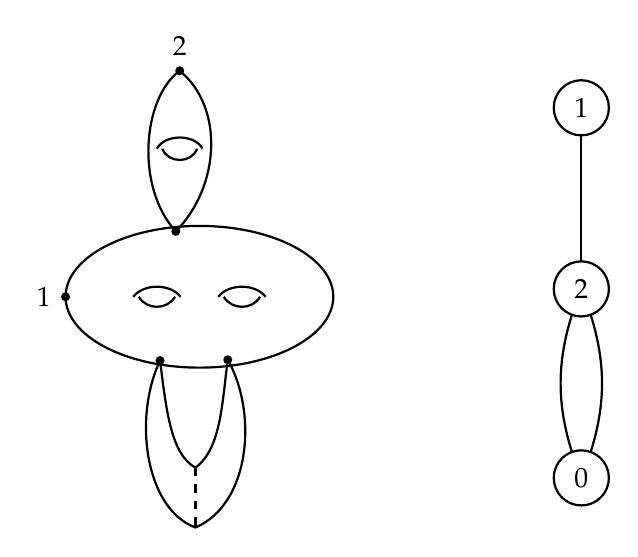
\begin{tikzpicture}[
        x=1cm,
        y=1cm,
        curve component/.style={thick},
        marked point/.style={circle,fill=black,inner sep=1.15pt},
        graph vertex/.style={
            circle,draw,thick,fill=white,minimum size=7mm,inner sep=0pt
        }
    ]
        % A three-component curve with components of genera 1, 2, and 0.
        \draw[curve component] (1.5,3.65) ellipse [x radius=1.7,y radius=0.9];

        % The two handles on the genus-two component.
        \draw[curve component]
            (0.66,3.65)
            .. controls (0.79,3.82) and (1.13,3.82) .. (1.26,3.65);
        \draw[curve component]
            (0.73,3.65)
            .. controls (0.83,3.48) and (1.09,3.48) .. (1.19,3.65);
        \draw[curve component]
            (1.74,3.65)
            .. controls (1.87,3.82) and (2.21,3.82) .. (2.34,3.65);
        \draw[curve component]
            (1.81,3.65)
            .. controls (1.91,3.48) and (2.17,3.48) .. (2.27,3.65);

        % The genus-one component attached above.
        \coordinate (uppernode) at (1.2,4.48);
        \draw[curve component]
            (uppernode)
            .. controls (0.68,5.05) and (0.78,6.18) .. (1.25,6.52)
            .. controls (1.82,6.05) and (1.76,5.05) .. cycle;
        \draw[curve component]
            (0.96,5.53)
            .. controls (1.06,5.72) and (1.44,5.72) .. (1.54,5.53);
        \draw[curve component]
            (1.03,5.53)
            .. controls (1.10,5.34) and (1.40,5.34) .. (1.47,5.53);

        % The rational component attached at two nodes below.
        \coordinate (lowerleft) at (1.00,2.84);
        \coordinate (lowerright) at (1.86,2.85);
        \draw[curve component]
            (lowerleft)
            .. controls (0.65,2.10) and (0.82,0.95) .. (1.45,0.72)
            .. controls (2.15,1.02) and (2.24,2.18) .. (lowerright);
        \draw[curve component]
            (lowerleft)
            .. controls (1.08,2.20) and (1.14,1.65) .. (1.45,1.48)
            .. controls (1.78,1.72) and (1.79,2.34) .. (lowerright);
        \draw[curve component,dashed] (1.45,1.48) -- (1.45,0.72);

        % Nodes and marked points.
        \node[marked point] at (uppernode) {};
        \node[marked point] at (lowerleft) {};
        \node[marked point] at (lowerright) {};
        \node[marked point,label=left:{$1$}] at (-0.2,3.65) {};
        \node[marked point,label=above:{$2$}] at (1.25,6.52) {};

        % The dual graph: the vertex labels record the genera.
        \coordinate (vone) at (6.35,6.05);
        \coordinate (vtwo) at (6.35,3.75);
        \coordinate (vzero) at (6.35,1.35);
        \draw[curve component] (vone) -- (vtwo);
        \draw[curve component]
            (vtwo) to[out=-112,in=112] (vzero);
        \draw[curve component]
            (vtwo) to[out=-68,in=68] (vzero);
        \node[graph vertex] at (vone) {$1$};
        \node[graph vertex] at (vtwo) {$2$};
        \node[graph vertex] at (vzero) {$0$};
    \end{tikzpicture}
    \end{center}
\end{exm}

For a log or punctured R-map
\begin{equation*}
\begin{tikzcd}
    & \mf{P} \ar{d} \\
    C \ar{ur}{f} \ar{d} \ar{r} & B \C_{\omega}^{\times} \\
    S,
\end{tikzcd}
\end{equation*}
we will tropicalize it by taking the associated generalized cone complex of the entire diagram. Because \(B \C_{\omega}^{\times}\) has no log structure, what we see is
\begin{equation*}
\begin{tikzcd}
    \Sigma(C) \ar{d} \ar{r}{\Sigma(f)} & \Sigma(\mf{P}) = \R_{\geq 0} \\
    \Sigma(S).
\end{tikzcd}
\end{equation*}
Now suppose that \(S = \Spec (Q \to \C)\) is a log point with \(Q\) an fs sharp monoid. In particular, this means that \(\Sigma(S) = Q_{\R}^{\vee}\). Because everything is (piecewise) linear, it suffices to consider an interior point \(t \in \Sigma(S)\) and consider \(\Sigma(C)_t\).

From each half edge, we treat it as pointing outward from the attached vertex, and in particular, this means that a linear map to \(\R_{\geq 0}\) corresponds to a slope. We will call these \textit{contact orders}. In particular, we have \(c(h) = - c(\hat{h})\) if \(h \neq \hat{h}\) are related by \(\imath\). For all \(v \in \V\), we also define the \textit{degeneracy}
\[ e_v \colon \Q_{\R}^{\vee} \to \R_{\geq 0} \qquad t \mapsto \Sigma(f)_t (v). \]
In particular, \(e_v \in Q\) is an integral point.

The next thing we need to introduce are punctured legs. They will be denoted by
\[ \L^{\circ} = \ab\{ h \in \H \mid \Sigma(f)_t(h) \text{ is bounded and nontrivial for all } t \in Q_{\R}^{\vee}\}. \] 
We will define prestability at \(h \in \L^{\circ}\) such that \(0 \in \ol{\Sigma(f)_t(h)}\), which is a technically necessary assumption. Under the assumption that all punctured legs are prestable, we can define the \textit{edge length} function
\[ \ell \colon \E \cup \L^{\circ} \to \ms{Map}(Q_{\R}^{\vee}, \R_{\geq 0}) \qquad x \mapsto \ell(x) \colon t \mapsto \ell(x)(t). \]
Note that \(\ell(E) \in Q\) is also an integral point for edges \(E\). For punctured legs, this is true up to subdivision.

\subsection{Log GLSM invariants}%
\label{sub:Log GLSM invariants}

\begin{defn}
    We will define the \textit{decorated tropical type} of a log map \(f\) as
    \[ \bm{\tau} = (G, c \colon \H \to \Z, \beta \colon \V \to H_2(X)). \]
\end{defn}

\begin{defn}
    A log or punctured map \(f\) is of \textit{compact type} if
    \begin{enumerate}
        \item \(\Ima \Sigma(f)_t\) is bounded for all \(t\);
        \item \(f(p_h) \in 0_{\mf{P}}\) for all half-edges \(h\) with contact order \(0\).
    \end{enumerate}
\end{defn}

We are now able to define the category \(\mc{R}(\mf{P}, \tau)\) of stable punctured R-maps fibered over the category \(\ms{LogSch}\) of fs log schemes and marked by \(\tau\).

\begin{thm}
    The stack \(\mc{R}(\mf{P},\bm{\tau})\) is represented by a proper DM stack with basic/minimal log structure.
\end{thm}

\begin{rmk}
    If \(\V = \ab\{v\}\) is a singleton, then we will write
    \[ \mc{R}_{g, c}(\mf{P}, \beta) \coloneqq \mc{R}(\mf{P}, \bm{\tau}). \]
\end{rmk}

Consider the diagram
\begin{equation*}
\begin{tikzcd}
    & \mf{P} \ar{d} \\
    \mc{C} \ar{ur}{f} \ar{d}{\pi} \ar{r} & B \C_{\omega}^{\times} \\
    \mc{R},
\end{tikzcd}
\end{equation*}
where we set \(\mc{R} \coloneqq \mc{R}(\mf{P}, \bm{\tau})\). Then the perfect obstruction theory is defined by
\[ T_{\mc{R}/\ms{Log}_{\mf{M}_G}} \to \E_{\square} = R \pi_* f^* T_{\mf{P}/B\C_{\omega}^{\times}}. \]
Here, both tangent bundles refer to the log tangent complex. From the perfect obstruction theory, this defines the canonical virtual cycle
\[ [\mc{R}(\mf{P}, \bm{\tau})]^{\vir}. \]
The main drawback of this virtual cycle is that it does not reproduce Gromov-Witten theory. However, we can consider how it differs from GW theory, but for this we need a birational modification. Let \(Q\) be a sharp monoid. It has a partial ordering by \(a < b\) if there exists a nonzero \(c \in Q\) such that \(a+c = b\).

\begin{defn}
    We say that either \(f\)  or \(\Sigma(f)\) has \textit{uniform maximal degeneracy} if there exists \(e_{\max} \in \ab\{e_v \mid v \in \V \}\) such that \(e_{\max} \geq e_v\) for all \(v \in \V\).
\end{defn}

\begin{rmk}
    If \(f\) is compact type and has uniform maximal degeneracy, then \(\Sigma(f)\) is uniformly bounded by \(e_{\max}\).
\end{rmk}

\begin{defn}
    Define \(\mc{U}(\mf{P}, \bm{\tau})\) to be the stack of stable punctured or log R-maps marked by \(\bm{\tau}\) with uniform maximal degeneracy.
\end{defn}

\begin{rmk}
    If \(\V = \ab\{v\}\) is a singleton, then we will write
    \[ \mc{U}_{g, c}(\mf{P}, \beta) \coloneqq \mc{U}(\mf{P}, \bm{\tau}). \]
    If one of the contact orders is negative, then we will write
    \[ \mc{U}_{g, c}(\infty, \beta) \coloneqq \mc{U}(\mf{P}, \bm{\tau}). \]
\end{rmk}

Note that there are two types of vertices: if a vertex is mapped to \(0\), then either there is at least one half-edge which points upwards or all contact orders are \(0\), in which case all are contracted. These are called \textit{log vertices}. The other type of vertex is one that does not go to \(0\). Either all half-edges point downwards, or there are some half-edges which point upwards. These are called \textit{\(\infty\)-vertices}. Moreover, the vertices which are compact types are the ones without upwards-pointing half-edges.

If we forget the condition of having uniform maximal degeneracy, then there is a map
\[ \mc{U}(\mf{P}, \bm{\tau}) \xrightarrow{F} \mc{R}(\mf{P}, \bm{\tau}) \]
which is a subcategory over \(\ms{LogSch}\). However, as a morphism of algebraic stacks, it is log \'etale, proper, and surjective. In addition, \(\mc{U}\) has a canonical perfect obstruction theory which is pulled back from \(\mc{R}\). In the case when the set of vertices is a singleton, we have
\begin{align*}
    F_* [\mc{U}_{g, c}(\mf{P}, \beta)]^{\vir} &= [\mc{R}_{g, c}(\mf{P}, \beta)]^{\vir}; \\
    F_* [\mc{U}_{g, c}(\infty, \beta)]^{\vir} &= [\mc{R}_{g, c}(\infty, \beta)]^{\vir}.
\end{align*}
In the case of a log vertex, we in fact have inclusions from the moduli of stable maps with p-fields as
\begin{equation*}
\begin{tikzcd}
    \mc{U} \ar{rr}{F} & & \mc{R} \\
    & \mc{R}_{g,c}(\mf{P}^{\circ}, \beta) \ar[hookrightarrow]{ul} \ar[hookrightarrow]{ur}.
\end{tikzcd}
\end{equation*}
If we denote the moduli of p-fields by \(\mc{R}^{\circ}\), then the boundary
\[ \Delta \coloneqq \mc{U} \setminus \mc{R}^{\circ} \]
is a Cartier divisor. By the condition of having uniform maximal degeneracy, we have a section
\[ e_{\max} \in H^0(\bar{M}_{\mc{U}}). \]
This is equivalent to the data of a morphism
\[ \mc{U} \to ([\A^1/\G_m], 0) \]
which pulls \(0\) back to \(\Delta\).

We will define a \textit{superpotential} to be a function
\begin{equation*}
\begin{tikzcd}
    \mf{P}^{\circ} \ar{rr}{W} \ar{dr} && \mc{L}_{\omega} \ar{dl} \\
    & B \C_{\times}^{\omega}.
\end{tikzcd}
\end{equation*}
Its \textit{critical locus} is denoted by 
\[ \on{Crit}(W) = (\d{W} = 0). \]
We say that \(W\) has \textit{proper critical locus} if \(\on{Crit}(W) \to B\C_{\omega}^{\times}\) is proper.

For example, suppose we are interested in GW theory. Let \(X\) be a smooth projective variety, \(V\) be a vector bundle on \(X\), and \(s \in H^0(V)\). Set \(Z = (s = 0)\). Then we obtain
\[ W \colon \mf{P}^{\circ} = V^{\vee} \boxtimes \mc{L}_{\omega} \xrightarrow{s \otimes 1_{\omega}} \mc{L}_{\omega}. \]

\begin{lem}
    \(W\) has proper critical locus if and only if \(Z\) is smooth of expected codimension.
\end{lem}

\begin{exm}
    Let \(X\) be a point, \(V = \C\), and \(s \neq 0\). Then \(\d{W} = s \neq 0\), so the critical locus is empty.
\end{exm}

Using the Kiem-Li method of cosection localization, we can obtain a virtual cycle
\[ [\mc{R}_{G, c=n}(\mf{P}^{\circ}, \beta)]_W^{\vir}, \]
which is supported on the critical locus. In GW theory, this equals the GW virtual cycle, 
\[ \pm [\bar{M}_{g,n}(\on{Crit}(W), \beta)]^{\vir}, \]
where the sign can be explicitly calculated.

\begin{thm}
    Let \(\bm{\tau}\) be a of compact type. In the compact type setting, 
    \begin{enumerate}
        \item \(\mc{U}(\mf{P}, \bm{\tau})\) has a reduced perfect obstruction theory, which yields a reduced virtual cycle \([\mc{U}(\mf{P}, \bm{\tau})]^{\vir}\);
        \item \(\Delta\) has a reduced perfect obstruction theory, which yields a reduced virtual cycle \([\Delta]^{\vir}\);
        \item We have \([\mc{U}_{g, c=n}(\mf{P}, \beta)]^{\on{red}} = \pm [\bar{M}_{g,n}(\on{Crit}(W), \beta)]^{\vir}\) in the case of a single log vertex. Moreover, there is the formula
            \[ [\mc{U}_{g, c=n}(\mf{P}, \beta)]^{\on{red}} = [\mc{U}_{g, c=n}(\mf{P}, \beta)]^{\vir} - \tilde{r} [\Delta]^{\on{red}}, \]
            where \(\tilde{r}\) is the pole order of \(W\) along \(\infty\).
    \end{enumerate}
\end{thm}

\subsection{Tropical decomposition and finite generation}%
\label{sub:Tropical decomposition and finite generation}

From now on, we will consider a simpler setup where \(X\) is a smooth projetive variety and \(V\) is a line bundle on \(X\). In this case, we will assume that \(Z = (s = 0)\) is smooth of codimension \(1\). Moreover, we will assume that \(Z\) is a Calabi-Yau threefold. We will consider the invariants
\[ N_{g, \beta} \coloneqq \int_{[\bar{M}_{g,0}(Z, \beta)]^{\vir}} 1 \in \Q \]
and the generating series
\[ F_g = \sum_{\beta \geq 0} N_{g, \beta} Q^{\beta} \in \Lambda \coloneqq \C \ps{Q}. \]

\begin{conj}[Yamaguchi-Yau, Alim-L\"ange]
    Suppose \(g=0\) mirror symmetry holds for \(Z\). Then there exists a finitely-generated \(\Q\)-algebra \(R \subset \Lambda'\) such that for all \(g \geq 2\), \(F_g \in (I_0(q))^{2g-2} R\).
\end{conj}

Our main goal is the following.

\begin{thm}
    Let \(Z\) be a Calabi-Yau threefold hypersurface in a Fano fourfold \(X\) with no odd cohomology. Let \(\{\phi_j\}\) be a basis of \(H^*(X)\) and \(\ab\{\phi^j\}\) be the dual basis. Then for all \(g \geq 0\), we have
    \begin{align*}
        &F_g = (-1)^{1-g} \sum_{\tau' \in G_g'} \frac{(-1)^{\abs{\V_{\infty}}}}{\Aut(\tau')} \cdot \prod_{E \in \E} c(E) \\
        & \cdot \sum_{j_E \mid E = \ab\{E_{\log}, E_{\infty}\} \in \E} \prod_{\substack{v \in \V_{\infty} \\ g=1 \\ \H_v = \ab\{E_{\infty}\}}} c_1^{\mr{eff}}(\phi^{j_E}) \cdot \prod_{\substack{v \in \V_{\infty} \\ g(v) \geq 2}} \tilde{Q}^{\beta(v)} \cdot \exp \ab(\int_{\beta(v)} K(Q) )  \\
        & \cdot \ab(\prod_{E_{\infty} \in \H_v'}\int \beta(v)\phi^{j_E}) \cdot c_{g(v), \beta(v)}^{\on{eff}} 
         \cdot \prod_{v \in \V_{\log}} \Omega_{g(v), \abs{\H_1(v)}, \abs{\H_2(v)}} (\phi_{j_E} \colon E_{\log} \in \H_1(v)).
    \end{align*}
\end{thm}

\begin{exm}
    Let \(Y\) be a toric variety with its toric log structure. Then \(\Sigma(Y)\) is the toric fan treated as a cone complex, and we can consider its boundary \(\Delta_Y = \sum_{\rho \in \Sigma(Y)^1} \Delta_{\rho}\). 
\end{exm}

If we consider \([\Delta]^{\on{red}}\), we should obtain the similar formula
\[ [\Delta]^{\on{red}} = \sum_{\rho \in \Sigma(\Delta)(1)} [\Delta_{\rho}]^{\on{red}}. \]
The question now is what the \(\rho\) represent. In fact, they parameterize rigid tropical curves. In the tropicalization
\begin{equation*}
\begin{tikzcd}
    \Sigma(C)_{\rho} \ar{d} \ar{r} & \Sigma(\mc{C}) \ar{r}{f} \ar{d} & \R_{\geq 0} \\
    \rho \ar[hookrightarrow]{r} & \Sigma(\mc{U}),
\end{tikzcd}
\end{equation*}
we see that \(f_{\rho}\) is rigid if and only if the source tropical curve is a bipartite graph with one set of vertives going to \(e_{\max}\) and the other set of vertices going to \(0\).

\begin{exm}
    Let \(X\) be a point and \(Z = \emptyset\). Also consider \(g = 2, n = 0\). Then the possible graphs are given in~\Cref{fig:tropgraphs}.
    \begin{figure}[htpb]
    \begin{center}
    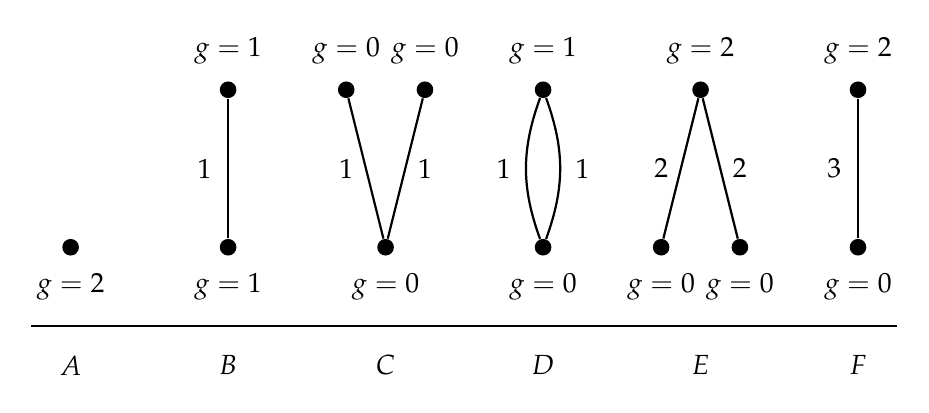
\begin{tikzpicture}[scale=1, transform shape]
        \node[fill=black,circle,minimum size=6pt,inner sep=0pt] (A) at (0,0) {};
        \node[fill=black,circle,minimum size=6pt,inner sep=0pt] (B1) at (2,0) {};
        \node[fill=black,circle,minimum size=6pt,inner sep=0pt] (B2) at (2,2) {};
        \node[fill=black,circle,minimum size=6pt,inner sep=0pt] (C1) at (4,0) {};
        \node[fill=black,circle,minimum size=6pt,inner sep=0pt] (C2) at (3.5,2) {};
        \node[fill=black,circle,minimum size=6pt,inner sep=0pt] (C3) at (4.5,2) {};
        \node[fill=black,circle,minimum size=6pt,inner sep=0pt] (D1) at (6,0) {};
        \node[fill=black,circle,minimum size=6pt,inner sep=0pt] (D2) at (6,2) {};
        \node[fill=black,circle,minimum size=6pt,inner sep=0pt] (E1) at (8,2) {};
        \node[fill=black,circle,minimum size=6pt,inner sep=0pt] (E2) at (7.5,0) {};
        \node[fill=black,circle,minimum size=6pt,inner sep=0pt] (E3) at (8.5,0) {};
        \node[fill=black,circle,minimum size=6pt,inner sep=0pt] (F1) at (10,0) {};
        \node[fill=black,circle,minimum size=6pt,inner sep=0pt] (F2) at (10,2) {};
        \draw[-,thick] (B1) -- (B2);
        \draw[-,thick] (C2) -- (C1) -- (C3);
        \draw[-,thick] (D1) edge[bend left=20] (D2);
        \draw[-,thick] (D2) edge[bend left=20] (D1);
        \draw[-,thick] (E2) -- (E1) -- (E3);
        \draw[-,thick] (F1) -- (F2);
        \node at (0,-0.5) {$g=2$};
        \node at (2,-0.5) {$g=1$};
        \node at (4,-0.5) {$g=0$};
        \node at (6,-0.5) {$g=0$};
        \node at (7.5,-0.5) {$g=0$};
        \node at (8.5,-0.5) {$g=0$};
        \node at (10,-0.5) {$g=0$};
        \node at (2,2.5) {$g=1$};
        \node at (3.5,2.5) {$g=0$};
        \node at (4.5,2.5) {$g=0$};
        \node at (6,2.5) {$g=1$};
        \node at (8,2.5) {$g=2$};
        \node at (10,2.5) {$g=2$};
        \draw[-,thick] (-0.5,-1) -- (10.5,-1);
        \node at (0,-1.5) {$A$};
        \node at (2,-1.5) {$B$};
        \node at (4,-1.5) {$C$};
        \node at (6,-1.5) {$D$};
        \node at (8,-1.5) {$E$};
        \node at (10,-1.5) {$F$};
        \node at (1.7,1) {$1$};
        \node at (3.5,1) {$1$};
        \node at (4.5,1) {$1$};
        \node at (5.5,1) {$1$};
        \node at (6.5,1) {$1$};
        \node at (7.5,1) {$2$};
        \node at (8.5,1) {$2$};
        \node at (9.7,1) {$3$};
    \end{tikzpicture}
    \end{center}
        \caption{Graphs of tropical types for $X = \mr{pt}$ and \(Z = \emptyset\) when $g=2$.}%
    \label{fig:tropgraphs}
    \end{figure}
\end{exm}

\begin{thm}[Tropical quantum Lefschetz]
    Let \(X\) and \(Z\) be as before. For any \(\beta \in H_2(X)\), any \(\alpha_1, \ldots, \alpha_n \in H^*(X)\), and any \(k_1, \ldots, k_n \in \N\), we have
    \begin{align*}
        \int_{[\bar{M}_{g,n}(Z,\beta)]^{\vir}} \prod_{j=1}^n \ev_j^* (\alpha_j) \psi^{k_j}={}& (-1)^{1-g+\beta \cdot Z} \cdot \prod_{\tau \vdash (g,n,\beta)} \frac{(-1)^{\abs{\V_{\infty}}}}{\abs{\Aut(\tau)}} \cdot \prod_{E \in \E} c(E) \\
        & \cdot \sum_{\ab\{j_E \mid E = \ab\{E_{\log}, E_{\infty}\}\}}  \prod_{v \in \V_{\infty}} \int_{[\mc{U}_v]^{\on{red}}} \prod_{E_{\infty} \in \H_v} \ev_{E_{\infty}}^* \phi^{j_E}  \\
        &  \cdot \prod_{v \in \V_{\log}} \int_{[\mc{R}_v]^{\vir}} \prod_{E_{\log}} \ev_{E_{\log}}^* (\phi_{j_E}) \cdot \prod_{h \in \L_v} \ev_h^* \alpha_h \cdot \psi_h^{k_n} .
    \end{align*}
\end{thm}

\begin{rmk}
    There is also a virtual localization formula, which can be applied to either the reduced theory (with only the R-torus action) or the canonical theory (which can be applied to the full automorphisms of the ambient space).
\end{rmk}

Now consider an \(\infty\)-vertex. Set \(\tau_v = (g, c, \beta)\) and set \(\mc{U}_v = \mc{U}_{g,c}(\infty, \beta)\). Then the first computation is that
\begin{align*}
    \on{red}\dim \mc{U}_v &= \chi(f^* T_{\mf{P}/B \C^{\times}_{\omega}}) + 1 + \on{trop}\dim  \\
    &= \vir\dim \bar{M}_{g,n}(Z, \beta) + \sum_{h \in \H} (c(h) + 1),
\end{align*}
where the tropical dimension is \(3g-4+n\). Note that all contact orders are negative, so the second term is at most zero. In particular, we have proved that
\begin{cor}
    If \(\vir\dim \bar{M}_{g,n}(Z,\beta) < 0\), then \([\mc{U}_v]^{\on{red}} = 0\).
\end{cor}
We also have an \textit{balancing condition}, which states that 
\[ \sum_{h \in \H} c(h) = \deg f^* \mc{O}(\infty) = \int_{\beta} c_1(V) - (2g-2+n). \]
This can be rewritten as
\[ 0 \geq \sum_{h \in \H} (c(h)+1) = \int_{\beta} c_1(V) - (2g-2). \]
\begin{prop}
    We see that \(\infty\)-vertices do not exist in the following cases:
    \begin{enumerate}
        \item We have \(g = 0\) and \(V\) is nef;
        \item We have \(g=1\) and \(V\) is ample, unless \(\beta = 0\) and all \(c(h) = -1\).
    \end{enumerate}
\end{prop}

\begin{defn}
    A marking is a \textit{unit} if its contact order is \(-1\).
\end{defn}

\begin{notn}
    We will denote the unit sector by \(\1\) and denote \(\tau_{v+\1} = (g, c+\1, \beta)\), \(\mc{U}_{v+\1} = U_{g, c+\1}(\infty, \beta)\), and \(\mc{R}_{v+\1} = \mc{R}_{g, c+\1}(\infty, \beta)\).
\end{notn}

\begin{thm}\leavevmode
    \begin{enumerate}
        \item There is a map \(F_{\1} \colon \mc{U}_{v+\1} \xrightarrow{s} \mc{C}^{\circ} \xrightarrow{\pi} \mc{U}_v\), where \(s\) is birational;
        \item We have the equality \(s_* [\mc{U}_{v+\1}]^{\on{red}} = \pi^* [\mc{U}_v]^{\on{red}}\) of reduced virtual cycles;
        \item If \(D\) is a divisor on \(X\), then \(F_{\1 *} (\ev_{\1}^* D \cap [\mc{U}_{v+\1}]^{\on{red}}) = \ab(\int_{\beta} D) [\mc{U}_v]^{\on{red}}\); 
        \item Consider the diagram
            \begin{equation*}
            \begin{tikzcd}
                \mc[U]_{v+\1} \ar{r}{F} \ar{d}[swap]{F_{\1}} & \bar{M}_{g,n+1} \ar{d}[swap]{p} \\
                \mc{U}_v \ar{r}{F} & \bar{M}_{g,n}.
            \end{tikzcd}
            \end{equation*}
            Then \(F_* [\mc{U}_{v+\1}]^{\on{red}} = p^* F_* [\mc{U}_v]^{\on{red}}\).
    \end{enumerate}
\end{thm}

\begin{exm}
    Consider the setting where \(g = 1\) and \(Z_d \subset X = \P^N\) is a hypersurface. We only need to consider \(\beta = 0\) and \(c(h) = -1\) for all \(h \in H\). Then we see that
    \[ \prod_h \ev_h^* \alpha_h \cdot [\mc{U}_{1,c}(\infty,\beta)]^{\mr{red}} = \ev_{h^{\star}}^* \ab(\prod_h \alpha_h) \cap [\mc{U}_{1,\1}(\infty,\beta)]^{\on{red}}. \]
\end{exm}

\begin{prop}
    We in fact have
    \[ \mc{U}_{1,\1}(\infty, 0) \simeq \mc{R}_{1,\1}(\infty, 0) \]
    and the equality
    \[ [\mc{U}_{1,\1}(\infty, 0)]^{\on{red}} = c_{\dim X} \ab(\mc{H}^{\vee} \boxtimes T_{\mf{P}/B\C_{\omega}^{\times}} + \mc{O} - V). \]
\end{prop}

\begin{exm}
    Now consider the quintic threefold \(Z_5 \subset \P^4\). Then we see that \(\on{red}\dim \mc{U}_v = \sum_{h \in \H} (c(h)+2)\). The unit axiom reduces us to the case when \(c(h) \leq -2\). We must now determine the number of new invariants we need to consider if all \(c(h) = -2\), which is equivalent to finding the number of possible \(\beta\). The balancing condition states that
    \begin{align*}
        \sum_{h \in \H} c(h) &= \int_{\beta} c_1(V) - (2g-2+n) \\
        &= 5\beta - (2g-2+n),
    \end{align*}
    which implies that \(0 \geq \sum (c(h)+1) = 5\beta - (2g-2)\) and therefore that \(\beta \leq \frac{2g-2}{5}\).\footnote{This is exactly the number of unknowns predicted if we assume finite generation, the holomorphic anomaly equations, orbifold regularity, and the conifold gap condition.}
\end{exm}

\begin{conj}[Janda]\leavevmode
    \begin{enumerate}
        \item We have \(K(Q) = \log I_0(q) \cdot c_1(K_X^{\vee}) - \frac{I_1}{I_0}\) \\
        \item The canonical theory satisfies \(\Omega \in I_0(q)^{2g-2+2n_1 + 3 n_2} \cdot R\). 
    \end{enumerate}
\end{conj}

\begin{cor}
    The above conjecture for \((X, V)\) implies Yamaguchi-Yau finite generation for \(Z\).
\end{cor}
















\end{document}

%%% Local Variables:
%%% mode: latex
%%% TeX-master: t
%%% End:
